% Options for packages loaded elsewhere
\PassOptionsToPackage{unicode}{hyperref}
\PassOptionsToPackage{hyphens}{url}
\PassOptionsToPackage{dvipsnames,svgnames,x11names}{xcolor}
%
\documentclass[
  letterpaper,
  DIV=11,
  numbers=noendperiod]{scrreprt}

\usepackage{amsmath,amssymb}
\usepackage{iftex}
\ifPDFTeX
  \usepackage[T1]{fontenc}
  \usepackage[utf8]{inputenc}
  \usepackage{textcomp} % provide euro and other symbols
\else % if luatex or xetex
  \usepackage{unicode-math}
  \defaultfontfeatures{Scale=MatchLowercase}
  \defaultfontfeatures[\rmfamily]{Ligatures=TeX,Scale=1}
\fi
\usepackage{lmodern}
\ifPDFTeX\else  
    % xetex/luatex font selection
\fi
% Use upquote if available, for straight quotes in verbatim environments
\IfFileExists{upquote.sty}{\usepackage{upquote}}{}
\IfFileExists{microtype.sty}{% use microtype if available
  \usepackage[]{microtype}
  \UseMicrotypeSet[protrusion]{basicmath} % disable protrusion for tt fonts
}{}
\makeatletter
\@ifundefined{KOMAClassName}{% if non-KOMA class
  \IfFileExists{parskip.sty}{%
    \usepackage{parskip}
  }{% else
    \setlength{\parindent}{0pt}
    \setlength{\parskip}{6pt plus 2pt minus 1pt}}
}{% if KOMA class
  \KOMAoptions{parskip=half}}
\makeatother
\usepackage{xcolor}
\setlength{\emergencystretch}{3em} % prevent overfull lines
\setcounter{secnumdepth}{5}
% Make \paragraph and \subparagraph free-standing
\makeatletter
\ifx\paragraph\undefined\else
  \let\oldparagraph\paragraph
  \renewcommand{\paragraph}{
    \@ifstar
      \xxxParagraphStar
      \xxxParagraphNoStar
  }
  \newcommand{\xxxParagraphStar}[1]{\oldparagraph*{#1}\mbox{}}
  \newcommand{\xxxParagraphNoStar}[1]{\oldparagraph{#1}\mbox{}}
\fi
\ifx\subparagraph\undefined\else
  \let\oldsubparagraph\subparagraph
  \renewcommand{\subparagraph}{
    \@ifstar
      \xxxSubParagraphStar
      \xxxSubParagraphNoStar
  }
  \newcommand{\xxxSubParagraphStar}[1]{\oldsubparagraph*{#1}\mbox{}}
  \newcommand{\xxxSubParagraphNoStar}[1]{\oldsubparagraph{#1}\mbox{}}
\fi
\makeatother

\usepackage{color}
\usepackage{fancyvrb}
\newcommand{\VerbBar}{|}
\newcommand{\VERB}{\Verb[commandchars=\\\{\}]}
\DefineVerbatimEnvironment{Highlighting}{Verbatim}{commandchars=\\\{\}}
% Add ',fontsize=\small' for more characters per line
\usepackage{framed}
\definecolor{shadecolor}{RGB}{241,243,245}
\newenvironment{Shaded}{\begin{snugshade}}{\end{snugshade}}
\newcommand{\AlertTok}[1]{\textcolor[rgb]{0.68,0.00,0.00}{#1}}
\newcommand{\AnnotationTok}[1]{\textcolor[rgb]{0.37,0.37,0.37}{#1}}
\newcommand{\AttributeTok}[1]{\textcolor[rgb]{0.40,0.45,0.13}{#1}}
\newcommand{\BaseNTok}[1]{\textcolor[rgb]{0.68,0.00,0.00}{#1}}
\newcommand{\BuiltInTok}[1]{\textcolor[rgb]{0.00,0.23,0.31}{#1}}
\newcommand{\CharTok}[1]{\textcolor[rgb]{0.13,0.47,0.30}{#1}}
\newcommand{\CommentTok}[1]{\textcolor[rgb]{0.37,0.37,0.37}{#1}}
\newcommand{\CommentVarTok}[1]{\textcolor[rgb]{0.37,0.37,0.37}{\textit{#1}}}
\newcommand{\ConstantTok}[1]{\textcolor[rgb]{0.56,0.35,0.01}{#1}}
\newcommand{\ControlFlowTok}[1]{\textcolor[rgb]{0.00,0.23,0.31}{\textbf{#1}}}
\newcommand{\DataTypeTok}[1]{\textcolor[rgb]{0.68,0.00,0.00}{#1}}
\newcommand{\DecValTok}[1]{\textcolor[rgb]{0.68,0.00,0.00}{#1}}
\newcommand{\DocumentationTok}[1]{\textcolor[rgb]{0.37,0.37,0.37}{\textit{#1}}}
\newcommand{\ErrorTok}[1]{\textcolor[rgb]{0.68,0.00,0.00}{#1}}
\newcommand{\ExtensionTok}[1]{\textcolor[rgb]{0.00,0.23,0.31}{#1}}
\newcommand{\FloatTok}[1]{\textcolor[rgb]{0.68,0.00,0.00}{#1}}
\newcommand{\FunctionTok}[1]{\textcolor[rgb]{0.28,0.35,0.67}{#1}}
\newcommand{\ImportTok}[1]{\textcolor[rgb]{0.00,0.46,0.62}{#1}}
\newcommand{\InformationTok}[1]{\textcolor[rgb]{0.37,0.37,0.37}{#1}}
\newcommand{\KeywordTok}[1]{\textcolor[rgb]{0.00,0.23,0.31}{\textbf{#1}}}
\newcommand{\NormalTok}[1]{\textcolor[rgb]{0.00,0.23,0.31}{#1}}
\newcommand{\OperatorTok}[1]{\textcolor[rgb]{0.37,0.37,0.37}{#1}}
\newcommand{\OtherTok}[1]{\textcolor[rgb]{0.00,0.23,0.31}{#1}}
\newcommand{\PreprocessorTok}[1]{\textcolor[rgb]{0.68,0.00,0.00}{#1}}
\newcommand{\RegionMarkerTok}[1]{\textcolor[rgb]{0.00,0.23,0.31}{#1}}
\newcommand{\SpecialCharTok}[1]{\textcolor[rgb]{0.37,0.37,0.37}{#1}}
\newcommand{\SpecialStringTok}[1]{\textcolor[rgb]{0.13,0.47,0.30}{#1}}
\newcommand{\StringTok}[1]{\textcolor[rgb]{0.13,0.47,0.30}{#1}}
\newcommand{\VariableTok}[1]{\textcolor[rgb]{0.07,0.07,0.07}{#1}}
\newcommand{\VerbatimStringTok}[1]{\textcolor[rgb]{0.13,0.47,0.30}{#1}}
\newcommand{\WarningTok}[1]{\textcolor[rgb]{0.37,0.37,0.37}{\textit{#1}}}

\providecommand{\tightlist}{%
  \setlength{\itemsep}{0pt}\setlength{\parskip}{0pt}}\usepackage{longtable,booktabs,array}
\usepackage{calc} % for calculating minipage widths
% Correct order of tables after \paragraph or \subparagraph
\usepackage{etoolbox}
\makeatletter
\patchcmd\longtable{\par}{\if@noskipsec\mbox{}\fi\par}{}{}
\makeatother
% Allow footnotes in longtable head/foot
\IfFileExists{footnotehyper.sty}{\usepackage{footnotehyper}}{\usepackage{footnote}}
\makesavenoteenv{longtable}
\usepackage{graphicx}
\makeatletter
\def\maxwidth{\ifdim\Gin@nat@width>\linewidth\linewidth\else\Gin@nat@width\fi}
\def\maxheight{\ifdim\Gin@nat@height>\textheight\textheight\else\Gin@nat@height\fi}
\makeatother
% Scale images if necessary, so that they will not overflow the page
% margins by default, and it is still possible to overwrite the defaults
% using explicit options in \includegraphics[width, height, ...]{}
\setkeys{Gin}{width=\maxwidth,height=\maxheight,keepaspectratio}
% Set default figure placement to htbp
\makeatletter
\def\fps@figure{htbp}
\makeatother
% definitions for citeproc citations
\NewDocumentCommand\citeproctext{}{}
\NewDocumentCommand\citeproc{mm}{%
  \begingroup\def\citeproctext{#2}\cite{#1}\endgroup}
\makeatletter
 % allow citations to break across lines
 \let\@cite@ofmt\@firstofone
 % avoid brackets around text for \cite:
 \def\@biblabel#1{}
 \def\@cite#1#2{{#1\if@tempswa , #2\fi}}
\makeatother
\newlength{\cslhangindent}
\setlength{\cslhangindent}{1.5em}
\newlength{\csllabelwidth}
\setlength{\csllabelwidth}{3em}
\newenvironment{CSLReferences}[2] % #1 hanging-indent, #2 entry-spacing
 {\begin{list}{}{%
  \setlength{\itemindent}{0pt}
  \setlength{\leftmargin}{0pt}
  \setlength{\parsep}{0pt}
  % turn on hanging indent if param 1 is 1
  \ifodd #1
   \setlength{\leftmargin}{\cslhangindent}
   \setlength{\itemindent}{-1\cslhangindent}
  \fi
  % set entry spacing
  \setlength{\itemsep}{#2\baselineskip}}}
 {\end{list}}
\usepackage{calc}
\newcommand{\CSLBlock}[1]{\hfill\break\parbox[t]{\linewidth}{\strut\ignorespaces#1\strut}}
\newcommand{\CSLLeftMargin}[1]{\parbox[t]{\csllabelwidth}{\strut#1\strut}}
\newcommand{\CSLRightInline}[1]{\parbox[t]{\linewidth - \csllabelwidth}{\strut#1\strut}}
\newcommand{\CSLIndent}[1]{\hspace{\cslhangindent}#1}

\usepackage{booktabs}
\usepackage{caption}
\usepackage{longtable}
\usepackage{colortbl}
\usepackage{array}
\usepackage{anyfontsize}
\usepackage{multirow}
\KOMAoption{captions}{tableheading}
\makeatletter
\@ifpackageloaded{bookmark}{}{\usepackage{bookmark}}
\makeatother
\makeatletter
\@ifpackageloaded{caption}{}{\usepackage{caption}}
\AtBeginDocument{%
\ifdefined\contentsname
  \renewcommand*\contentsname{Table of contents}
\else
  \newcommand\contentsname{Table of contents}
\fi
\ifdefined\listfigurename
  \renewcommand*\listfigurename{List of Figures}
\else
  \newcommand\listfigurename{List of Figures}
\fi
\ifdefined\listtablename
  \renewcommand*\listtablename{List of Tables}
\else
  \newcommand\listtablename{List of Tables}
\fi
\ifdefined\figurename
  \renewcommand*\figurename{Figure}
\else
  \newcommand\figurename{Figure}
\fi
\ifdefined\tablename
  \renewcommand*\tablename{Table}
\else
  \newcommand\tablename{Table}
\fi
}
\@ifpackageloaded{float}{}{\usepackage{float}}
\floatstyle{ruled}
\@ifundefined{c@chapter}{\newfloat{codelisting}{h}{lop}}{\newfloat{codelisting}{h}{lop}[chapter]}
\floatname{codelisting}{Listing}
\newcommand*\listoflistings{\listof{codelisting}{List of Listings}}
\makeatother
\makeatletter
\makeatother
\makeatletter
\@ifpackageloaded{caption}{}{\usepackage{caption}}
\@ifpackageloaded{subcaption}{}{\usepackage{subcaption}}
\makeatother

\ifLuaTeX
  \usepackage{selnolig}  % disable illegal ligatures
\fi
\usepackage{bookmark}

\IfFileExists{xurl.sty}{\usepackage{xurl}}{} % add URL line breaks if available
\urlstyle{same} % disable monospaced font for URLs
\hypersetup{
  pdftitle={Mappeeksamen IDR4000},
  pdfauthor={Anders Nybakk},
  colorlinks=true,
  linkcolor={blue},
  filecolor={Maroon},
  citecolor={Blue},
  urlcolor={Blue},
  pdfcreator={LaTeX via pandoc}}


\title{Mappeeksamen IDR4000}
\author{Anders Nybakk}
\date{2024-11-22}

\begin{document}
\maketitle

\renewcommand*\contentsname{Table of contents}
{
\hypersetup{linkcolor=}
\setcounter{tocdepth}{2}
\tableofcontents
}

\bookmarksetup{startatroot}

\chapter*{Forord}\label{forord}
\addcontentsline{toc}{chapter}{Forord}

\markboth{Forord}{Forord}

https://github.com/Nybakk/mappeeksamen-idr4000-anders-nybakk

\bookmarksetup{startatroot}

\chapter{Reliabilitet og verktøy for reproduserbar vitenskapelig
data}\label{reliabilitet-og-verktuxf8y-for-reproduserbar-vitenskapelig-data}

\section{Introduksjon}\label{introduksjon}

I vår studie har vi gjennomført VO2 max-tester over fire forskjellige
dager for å vurdere påliteligheten av de innsamlede dataene. Formålet
med disse testene var å undersøke hvor konsistente resultatene er under
kontrollerte forhold. For å oppnå dette har vi forsøkt å standardisere
flere variabler, inkludert treningsnivå og matinntak dagen før testene.
Ifølge Halperin \emph{et al.} (2015) er det avgjørende å bruke
standardiserte protokoller for å oppnå pålitelige resultater i
fysiologiske tester. I tillegg har vi målt laktatnivåer umiddelbart
etter avslutningen av hver test for å vurdere den fysiologiske
responsen. Tidligere forskning har vist at laktatnivåer kan gi verdifull
informasjon om anaerob kapasitet og treningsintensitet, noe som er
viktig for å forstå atletisk ytelse (Hopkins (2000); Tanner \& Gore
(2012)). Ved å kontrollere for disse variablene håper vi å oppnå en høy
grad av reproduserbarhet i våre resultater.

I denne rapporten velger vi å fokusere på lakta-max og RER. Vi vil
sammenlikne disse, regne ut standard avvik.

\section{Protokoll}\label{protokoll}

Protokoll VO2maks-test

Vi gjennomførte fire testdager. De to første var påfølgende dager, og de
to siste var med en dag mellom. Hensikten med disse testdagene var å
gjennomføre fysiologiske tester med høy grad av reliabilitet. Det er
mange faktorer som kan påvirke validitet og reliabilitet, og det er
velidg viktig å ta høyde for dette under fysiologisk testing. Vi tok
flere forhåndsregler for å sikre så like testforhold som mulig.

En VO2maks-test går ut på å måle hvor mange ml en person evner å ta opp
og forbruke per minutt. Oksygenkravet øker lineært med økende belastning
helt til personen når sin maksimale aerobe kapasitet, da kurven enten
flater ut eller synker.

Maksimalt oksygenopptak beskrives enten i absolutte tall (ml/min) eller
som relative tall i forhold til kroppsvekt (ml/kg/min).

\subsection{Metode:}\label{metode}

VO2maks-testen ble gjennomført som en trappetrinnstest der motstanden
økte med 20W hvert minutt til utmattelse, eller når RPM \textless{} 60.
Det registreres målinger av VO2maks ved hvert 30 sek. Deltakerne startet
testen på en watt tilsvarende fysisk form og erfaring med sykkel. Etter
testene var ferdige ble informasjonen innhentet og plottet i et ferdig
formatert Excel-dokument.

Da en tydelig protokoll ble fulgt for å etterstrebe så sikre og reliable
tester som mulig, er det flere forhold som må tas underveis. Matinntak
og koffeininntak fra samme dag og kvelden før ble registrert ved første
test, og skulle være likt ved de påfølgende testene. Trening dagen før
test ble også registrert, men lyktes ikke i å reprodusere dette da
trening dagen før test 2 ble gårsdagens VO2maks-test. Vi hadde også
føringer om at man skulle etterstrebe lik søvn på dagene før test. For å
sikre lik grad av formuleringer og verbal instruks samt grad av
engasjement og heiing, hadde hver deltaker samme testleder ved hver
test.

\subsection{Protokoll}\label{protokoll-1}

\subsubsection{Før test:}\label{fuxf8r-test}

\begin{enumerate}
\def\labelenumi{\arabic{enumi}.}
\tightlist
\item
  Starte laktatmaskin
\item
  Bytte standard hvis den er tom (finnes i kjøleskap)
\item
  Finne frem munnstykke og sette sammen dette
\item
  Husk hansker
\item
  Papir med neseklype rundt når den er klar
\item
  Ta med ny slange som festes i miksekammer
\item
  Skru på Lode-sykkel.
\item
  Skru på Vyntus og Lode PC
\end{enumerate}

\textbf{Kalibrere oksygenanalysator}

\begin{enumerate}
\def\labelenumi{\arabic{enumi}.}
\tightlist
\item
  Gasskalibrering
\item
  Åpne gassflaske (lukkes når kalibrering er ferdig)
\item
  Sjekke at sensor er koblet i maskinen
\item
  Start kalibrering
\item
  Godtar 2\% feilmargin, hvis den er høyere må man rekalibrere
\item
  Volumkalibrering-
\item
  Feilmargin på 0,2\% eller under godtas
\item
  Kalibrere kammer
\item
  Flytte sensor til kammer
\item
  Skru av gass
\end{enumerate}

\textbf{Forberede utstyr}

\begin{enumerate}
\def\labelenumi{\arabic{enumi}.}
\item
  Lage ny pasient på Vyntus og Lode
\item
  Idr4000\_h24\_g1\_idx
\item
  Veie personen i så lite klær som mulig (trekke fra 300g for klær)
\item
  Lage plotteark
\item
  Stille inn krankarm (172,5) og kalibrere sykkel på Lode PC
\item
  Stille inn sykkel til deltaker
\item
  Fullføre plotteark
\item
  Klargjøre laktatrør, papir og teip, samt teip til neseklype
\item
  Velge protokoll på Lode PC. Dersom personen ikke har erfaring med
  sykkel må man bli enige om en Watt man tror kan passe.
\end{enumerate}

\textbf{Forklare forsøksperson hva testen innebærer, opplyse om borg
skala og hvor på skala man vil ha den.}

\begin{enumerate}
\def\labelenumi{\arabic{enumi}.}
\tightlist
\item
  VO2max -- Kondisjon
\item
  Målinger per 30 sek.
\item
  Prestasjonstest -- hvert sekund teller
\item
  Watt-økning per 1 min.
\item
  80-100 rpm, stopper test hvis under 60
\item
  Pulsmåling
\item
  Borg skala -- 6 = sofa, 20 = maks
\item
  Laktatmåling 1 min etter test -- stikk i fingeren
\item
  Vifte?
\end{enumerate}

\subsubsection{Etter test:}\label{etter-test}

\begin{enumerate}
\def\labelenumi{\arabic{enumi}.}
\tightlist
\item
  Avslutte test på begge PC
\item
  Spørre om Borg skala
\item
  1 minutt etter endt test skal det tas laktat-prøve. Tok 2 prøver for å
  sikre god reliabilitet.
\end{enumerate}

\textbf{Hente rapport:}

\begin{enumerate}
\def\labelenumi{\arabic{enumi}.}
\tightlist
\item
  Rapport: INN\_TABELL:30SEK\_MIX
\item
  Søke opp id-nr.
\item
  Lagre i rett mappe: F10 (nederste knapp)
\item
  Lagre i rett mappe på minnepenn
\item
  Overføre til One Drive på labbPCn
\end{enumerate}

\subsection{Standardisering:}\label{standardisering}

I dette forsøket valgte vi å standardisere matinntak og koffeininntak i
forkant av testen. Vi ønsket at testdeltakerne skulle spise det samme de
tre siste måltidene før testen, og ha likt koffeininntak samme dag som
testen.

Vi kunne også ha valgt å standardisere trening, men på grunn av
forskjellig treningsopplegg hos deltakerne lot ikke dette seg gjøre.

Standardisering av tidspunkt ble gjort for oss med reservasjon av
laboratorium 2. Helt standardisert blir det likevel ikke fordi i testuke
1 er testdagene rett etter hverandre, mens i testuke to er det en
hviledag mellom testene.

\section{Resultater}\label{resultater}

\begin{Shaded}
\begin{Highlighting}[]
\CommentTok{\# Last inn nødvendige biblioteker}
\FunctionTok{library}\NormalTok{(readxl)}
\FunctionTok{library}\NormalTok{(dplyr)}
\FunctionTok{library}\NormalTok{(tidyverse)}


\CommentTok{\# Definerer variablene som skal brukes}
\NormalTok{vars }\OtherTok{\textless{}{-}} \FunctionTok{c}\NormalTok{(}\StringTok{"id"}\NormalTok{, }\StringTok{"timepoint"}\NormalTok{, }\StringTok{"temperature"}\NormalTok{, }\StringTok{"humidity"}\NormalTok{, }
          \StringTok{"sex"}\NormalTok{, }\StringTok{"age"}\NormalTok{, }\StringTok{"height"}\NormalTok{, }\StringTok{"weight"}\NormalTok{, }\StringTok{"w.max"}\NormalTok{, }
          \StringTok{"vo2.max"}\NormalTok{, }\StringTok{"vco2.max"}\NormalTok{, }\StringTok{"rer.max"}\NormalTok{, }\StringTok{"ve.max"}\NormalTok{, }
          \StringTok{"bf.max"}\NormalTok{, }\StringTok{"hr.max"}\NormalTok{, }\StringTok{"la.max"}\NormalTok{, }
          \StringTok{"borg.max"}\NormalTok{)}

\CommentTok{\# Leser inn dataene fra Excel{-}filer og kombinerer dem}
\NormalTok{dat }\OtherTok{\textless{}{-}} \FunctionTok{bind\_rows}\NormalTok{(}
\FunctionTok{read\_excel}\NormalTok{(}\StringTok{"data/g1.xlsx"}\NormalTok{, }\AttributeTok{sheet =} \StringTok{"data\_excel"}\NormalTok{, }\AttributeTok{na =} \StringTok{"na"}\NormalTok{) }\SpecialCharTok{\%\textgreater{}\%}
  \FunctionTok{select}\NormalTok{(}\FunctionTok{all\_of}\NormalTok{(vars)) }\SpecialCharTok{\%\textgreater{}\%}
  \FunctionTok{mutate}\NormalTok{(}\AttributeTok{group =} \StringTok{"G1"}\NormalTok{, }
         \AttributeTok{id =} \FunctionTok{paste0}\NormalTok{(group, }\StringTok{"\_"}\NormalTok{, id)) ,}

\FunctionTok{read\_excel}\NormalTok{(}\StringTok{"data/g2.xlsx"}\NormalTok{, }\AttributeTok{na =} \StringTok{"na"}\NormalTok{) }\SpecialCharTok{\%\textgreater{}\%}
   \FunctionTok{select}\NormalTok{(}\FunctionTok{all\_of}\NormalTok{(vars)) }\SpecialCharTok{\%\textgreater{}\%}
  \FunctionTok{mutate}\NormalTok{(}\AttributeTok{group =} \StringTok{"G2"}\NormalTok{, }
         \AttributeTok{id =} \FunctionTok{paste0}\NormalTok{(group, }\StringTok{"\_"}\NormalTok{, id)) ,}

\FunctionTok{read\_excel}\NormalTok{(}\StringTok{"data/g3.xlsx"}\NormalTok{) }\SpecialCharTok{\%\textgreater{}\%}
   \FunctionTok{select}\NormalTok{(}\FunctionTok{all\_of}\NormalTok{(vars)) }\SpecialCharTok{\%\textgreater{}\%}
  \FunctionTok{mutate}\NormalTok{(}\AttributeTok{timepoint =} \FunctionTok{paste0}\NormalTok{(}\StringTok{"t"}\NormalTok{, timepoint), }
         \AttributeTok{group =} \StringTok{"G3"}\NormalTok{, }
         \AttributeTok{id =} \FunctionTok{paste0}\NormalTok{(group, }\StringTok{"\_"}\NormalTok{, id)) ,}

\FunctionTok{read\_excel}\NormalTok{(}\StringTok{"data/g4.xlsx"}\NormalTok{) }\SpecialCharTok{\%\textgreater{}\%}
   \FunctionTok{select}\NormalTok{(}\FunctionTok{all\_of}\NormalTok{(vars)) }\SpecialCharTok{\%\textgreater{}\%}
  \FunctionTok{mutate}\NormalTok{(}\AttributeTok{group =} \StringTok{"G4"}\NormalTok{, }
         \AttributeTok{id =} \FunctionTok{paste0}\NormalTok{(group, }\StringTok{"\_"}\NormalTok{, id)) )}


\CommentTok{\# Viser de første radene av det samlede datasettet}
\end{Highlighting}
\end{Shaded}

\subsection{Tabeller}\label{tabeller}

\emph{(n = antall deltagere).}

\subsubsection{Tabell over demografiske variabler
.}\label{tabell-over-demografiske-variabler-.}

\begin{Shaded}
\begin{Highlighting}[]
\NormalTok{dat }\SpecialCharTok{\%\textgreater{}\%}
  \FunctionTok{select}\NormalTok{(timepoint, age, height, weight) }\SpecialCharTok{\%\textgreater{}\%}
  \FunctionTok{group\_by}\NormalTok{(timepoint) }\SpecialCharTok{\%\textgreater{}\%}
  \FunctionTok{summarise}\NormalTok{(}
    \AttributeTok{m.age =} \FunctionTok{mean}\NormalTok{(age, }\AttributeTok{na.rm =} \ConstantTok{TRUE}\NormalTok{),}
    \AttributeTok{sd.age =} \FunctionTok{sd}\NormalTok{(age, }\AttributeTok{na.rm =} \ConstantTok{TRUE}\NormalTok{),}
    \AttributeTok{m.height =} \FunctionTok{mean}\NormalTok{(height, }\AttributeTok{na.rm =} \ConstantTok{TRUE}\NormalTok{),}
    \AttributeTok{sd.height =} \FunctionTok{sd}\NormalTok{(height, }\AttributeTok{na.rm =} \ConstantTok{TRUE}\NormalTok{),}
    \AttributeTok{m.weight =} \FunctionTok{mean}\NormalTok{(weight, }\AttributeTok{na.rm =} \ConstantTok{TRUE}\NormalTok{),}
    \AttributeTok{sd.weight =} \FunctionTok{sd}\NormalTok{(weight, }\AttributeTok{na.rm =} \ConstantTok{TRUE}\NormalTok{),}
    \AttributeTok{n =} \FunctionTok{n}\NormalTok{(),}
    \AttributeTok{.groups =} \StringTok{"drop"}
\NormalTok{  )}
\end{Highlighting}
\end{Shaded}

\begin{verbatim}
# A tibble: 4 x 8
  timepoint m.age sd.age m.height sd.height m.weight sd.weight     n
  <chr>     <dbl>  <dbl>    <dbl>     <dbl>    <dbl>     <dbl> <int>
1 t1         25.7   3.64     180.      7.63     79.2      11.9    14
2 t2         25.7   3.64     180.      7.63     79.3      11.8    14
3 t3         26.8   3.69     179.      7.91     80.4      11.9    11
4 t4         29.1   7.22     175.      6.16     74.7      12.3     8
\end{verbatim}

\begin{Shaded}
\begin{Highlighting}[]
\CommentTok{\# velger etter variablene, grupperer de etter timepoint(testdagene), summerer de forskjellige verdiene, n teller antall rader(deltagere) i hver gruppe }
\end{Highlighting}
\end{Shaded}

\subsubsection{Tabell over demografiske variabler fordelt etter
kjønn.}\label{tabell-over-demografiske-variabler-fordelt-etter-kjuxf8nn.}

\begin{Shaded}
\begin{Highlighting}[]
\NormalTok{dat }\SpecialCharTok{\%\textgreater{}\%}
  \FunctionTok{select}\NormalTok{(timepoint, sex, age, height, weight) }\SpecialCharTok{\%\textgreater{}\%}
  \FunctionTok{group\_by}\NormalTok{(timepoint, sex) }\SpecialCharTok{\%\textgreater{}\%}
  \FunctionTok{summarise}\NormalTok{(}
    \AttributeTok{m.age =} \FunctionTok{mean}\NormalTok{(age, }\AttributeTok{na.rm =} \ConstantTok{TRUE}\NormalTok{),}
    \AttributeTok{sd.age =} \FunctionTok{sd}\NormalTok{(age, }\AttributeTok{na.rm =} \ConstantTok{TRUE}\NormalTok{),}
    \AttributeTok{m.height =} \FunctionTok{mean}\NormalTok{(height, }\AttributeTok{na.rm =} \ConstantTok{TRUE}\NormalTok{),}
    \AttributeTok{sd.height =} \FunctionTok{sd}\NormalTok{(height, }\AttributeTok{na.rm =} \ConstantTok{TRUE}\NormalTok{),}
    \AttributeTok{m.weight =} \FunctionTok{mean}\NormalTok{(weight, }\AttributeTok{na.rm =} \ConstantTok{TRUE}\NormalTok{),}
    \AttributeTok{sd.weight =} \FunctionTok{sd}\NormalTok{(weight, }\AttributeTok{na.rm =} \ConstantTok{TRUE}\NormalTok{),}
    \AttributeTok{n =} \FunctionTok{n}\NormalTok{(),}
    \AttributeTok{.groups =} \StringTok{"drop"}
\NormalTok{  )}
\end{Highlighting}
\end{Shaded}

\begin{verbatim}
# A tibble: 8 x 9
  timepoint sex   m.age sd.age m.height sd.height m.weight sd.weight     n
  <chr>     <chr> <dbl>  <dbl>    <dbl>     <dbl>    <dbl>     <dbl> <int>
1 t1        f      23.9  0.569     171       8.19     71.7      9.90     3
2 t1        m      26.1  4.01      182.      5.72     81.2     11.9     11
3 t2        f      24.0  0.566     171       8.19     71.5      9.95     3
4 t2        m      26.1  4.01      182.      5.72     81.4     11.8     11
5 t3        f      24.2  0.389     168.      7.78     66.7      6.79     2
6 t3        m      27.4  3.88      181.      5.67     83.5     10.7      9
7 t4        f      30.7 11.2       168.      5.69     64.0      6.85     3
8 t4        m      28.1  4.97      178.      1.67     81.2     10.2      5
\end{verbatim}

variasjon eller reliabilitetstallet til den la.max, så den rer.max.
sammenlikne til slutt

\subsubsection{Standard avvik:}\label{standard-avvik}

\textbf{laktat}

\begin{Shaded}
\begin{Highlighting}[]
\NormalTok{dat }\SpecialCharTok{\%\textgreater{}\%}
  \FunctionTok{group\_by}\NormalTok{(timepoint) }\SpecialCharTok{\%\textgreater{}\%}
  \FunctionTok{summarise}\NormalTok{(}
    \AttributeTok{m =} \FunctionTok{mean}\NormalTok{(la.max, }\AttributeTok{na.rm =} \ConstantTok{TRUE}\NormalTok{),}
    \AttributeTok{s =} \FunctionTok{sd}\NormalTok{(la.max, }\AttributeTok{na.rm =} \ConstantTok{TRUE}\NormalTok{),}
     \AttributeTok{n =} \FunctionTok{n}\NormalTok{(),}
    \AttributeTok{.groups =} \StringTok{"drop"}\NormalTok{)}
\end{Highlighting}
\end{Shaded}

\begin{verbatim}
# A tibble: 4 x 4
  timepoint     m     s     n
  <chr>     <dbl> <dbl> <int>
1 t1         12.2  2.76    14
2 t2         12.3  2.91    14
3 t3         13.6  2.50    11
4 t4         13.8  2.31     8
\end{verbatim}

\textbf{laktat etter kjønn}

\begin{Shaded}
\begin{Highlighting}[]
\NormalTok{dat }\SpecialCharTok{\%\textgreater{}\%}
  \FunctionTok{group\_by}\NormalTok{(timepoint, sex) }\SpecialCharTok{\%\textgreater{}\%}
  \FunctionTok{summarise}\NormalTok{(}
    \AttributeTok{m =} \FunctionTok{mean}\NormalTok{(la.max, }\AttributeTok{na.rm =} \ConstantTok{TRUE}\NormalTok{),}
    \AttributeTok{s =} \FunctionTok{sd}\NormalTok{(la.max, }\AttributeTok{na.rm =} \ConstantTok{TRUE}\NormalTok{),}
     \AttributeTok{n =} \FunctionTok{n}\NormalTok{(),}
    \AttributeTok{.groups =} \StringTok{"drop"}\NormalTok{)}
\end{Highlighting}
\end{Shaded}

\begin{verbatim}
# A tibble: 8 x 5
  timepoint sex       m     s     n
  <chr>     <chr> <dbl> <dbl> <int>
1 t1        f      13.0 0.954     3
2 t1        m      12.0 3.08     11
3 t2        f      12.9 2.70      3
4 t2        m      12.1 3.09     11
5 t3        f      12   1.40      2
6 t3        m      14.0 2.60      9
7 t4        f      12.3 3.20      3
8 t4        m      14.7 1.15      5
\end{verbatim}

\textbf{RER}

\begin{Shaded}
\begin{Highlighting}[]
\NormalTok{dat }\SpecialCharTok{\%\textgreater{}\%}
  \FunctionTok{group\_by}\NormalTok{(timepoint) }\SpecialCharTok{\%\textgreater{}\%}
  \FunctionTok{summarise}\NormalTok{(}
    \AttributeTok{m =} \FunctionTok{mean}\NormalTok{(rer.max, }\AttributeTok{na.rm =} \ConstantTok{TRUE}\NormalTok{),}
    \AttributeTok{s =} \FunctionTok{sd}\NormalTok{(rer.max, }\AttributeTok{na.rm =} \ConstantTok{TRUE}\NormalTok{),}
     \AttributeTok{n =} \FunctionTok{n}\NormalTok{(),}
    \AttributeTok{.groups =} \StringTok{"drop"}
\NormalTok{  )}
\end{Highlighting}
\end{Shaded}

\begin{verbatim}
# A tibble: 4 x 4
  timepoint     m      s     n
  <chr>     <dbl>  <dbl> <int>
1 t1         1.14 0.0337    14
2 t2         1.15 0.0379    14
3 t3         1.18 0.0454    11
4 t4         1.19 0.0308     8
\end{verbatim}

\textbf{RER etter kjønn}

\begin{Shaded}
\begin{Highlighting}[]
\NormalTok{dat }\SpecialCharTok{\%\textgreater{}\%}
  \FunctionTok{group\_by}\NormalTok{(timepoint, sex) }\SpecialCharTok{\%\textgreater{}\%}
  \FunctionTok{summarise}\NormalTok{(}
    \AttributeTok{m =} \FunctionTok{mean}\NormalTok{(rer.max, }\AttributeTok{na.rm =} \ConstantTok{TRUE}\NormalTok{),}
    \AttributeTok{s =} \FunctionTok{sd}\NormalTok{(rer.max, }\AttributeTok{na.rm =} \ConstantTok{TRUE}\NormalTok{),}
     \AttributeTok{n =} \FunctionTok{n}\NormalTok{(),}
    \AttributeTok{.groups =} \StringTok{"drop"}
\NormalTok{  )}
\end{Highlighting}
\end{Shaded}

\begin{verbatim}
# A tibble: 8 x 5
  timepoint sex       m      s     n
  <chr>     <chr> <dbl>  <dbl> <int>
1 t1        f      1.14 0.0126     3
2 t1        m      1.14 0.0379    11
3 t2        f      1.16 0.0304     3
4 t2        m      1.14 0.0398    11
5 t3        f      1.17 0.0318     2
6 t3        m      1.18 0.0493     9
7 t4        f      1.19 0.0225     3
8 t4        m      1.18 0.0371     5
\end{verbatim}

\subsubsection{Graf over
laktatmålingene}\label{graf-over-laktatmuxe5lingene}

\begin{Shaded}
\begin{Highlighting}[]
\FunctionTok{ggplot}\NormalTok{(}\AttributeTok{data =}\NormalTok{ dat,}
       \FunctionTok{aes}\NormalTok{(}\AttributeTok{y =}\NormalTok{ la.max,}
           \AttributeTok{x =}\NormalTok{ timepoint,}
           \AttributeTok{group =}\NormalTok{ id)) }\SpecialCharTok{+}
  
  \FunctionTok{geom\_point}\NormalTok{() }\SpecialCharTok{+}
  
  \FunctionTok{geom\_line}\NormalTok{() }\SpecialCharTok{+} 
  
  \FunctionTok{labs}\NormalTok{(}\AttributeTok{y =} \StringTok{"laktate max (mmol)"}\NormalTok{,}
       \AttributeTok{x =} \StringTok{"tidspunkt (testnummer)"}\NormalTok{)}
\end{Highlighting}
\end{Shaded}

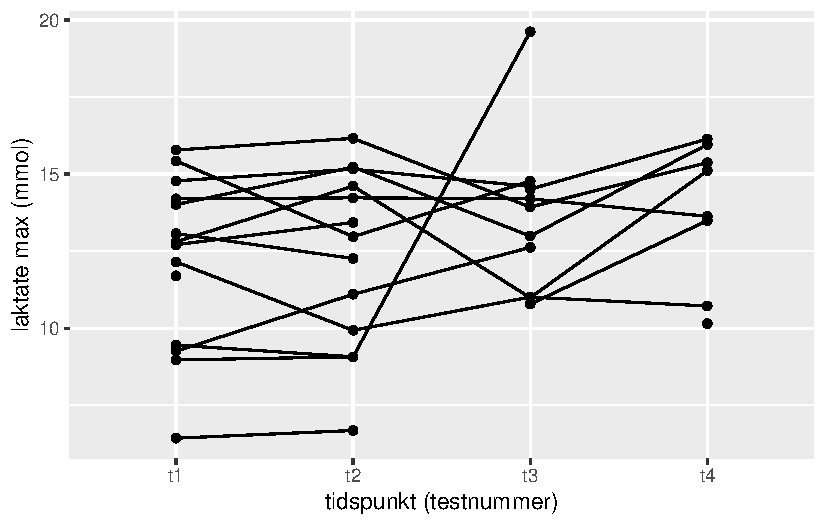
\includegraphics{Oppgave-1_files/figure-pdf/unnamed-chunk-8-1.pdf}

\subsubsection{Graf over
RER-målingene}\label{graf-over-rer-muxe5lingene}

\begin{Shaded}
\begin{Highlighting}[]
\FunctionTok{ggplot}\NormalTok{(}\AttributeTok{data =}\NormalTok{ dat,}
       \FunctionTok{aes}\NormalTok{(}\AttributeTok{y =}\NormalTok{ rer.max,}
           \AttributeTok{x =}\NormalTok{ timepoint,}
           \AttributeTok{group =}\NormalTok{ id)) }\SpecialCharTok{+}
  
  \FunctionTok{geom\_point}\NormalTok{() }\SpecialCharTok{+}
  
  \FunctionTok{geom\_line}\NormalTok{() }\SpecialCharTok{+} 
  
  \FunctionTok{labs}\NormalTok{(}\AttributeTok{y =} \StringTok{"RER max"}\NormalTok{,}
       \AttributeTok{x =} \StringTok{"tidspunkt (testnummer)"}\NormalTok{)}
\end{Highlighting}
\end{Shaded}

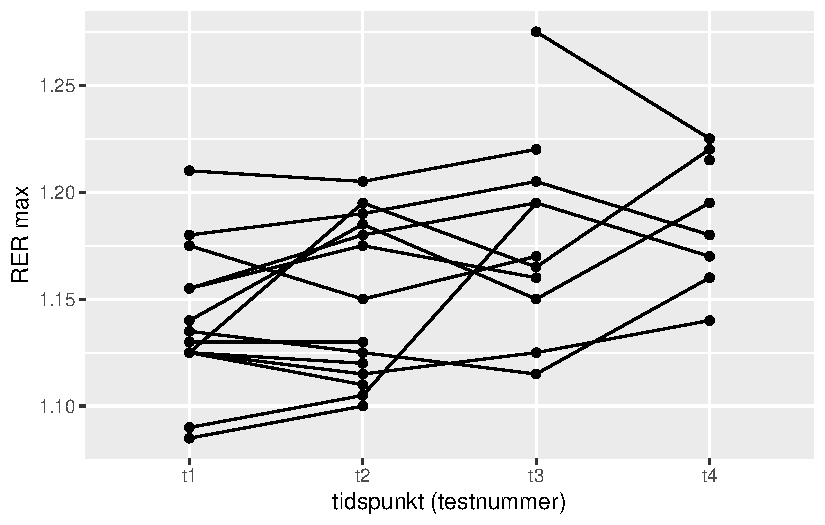
\includegraphics{Oppgave-1_files/figure-pdf/unnamed-chunk-9-1.pdf}

\section{Utregning av
variasjonskoeffisient}\label{utregning-av-variasjonskoeffisient}

\subsection{Laktat maks}\label{laktat-maks}

\begin{Shaded}
\begin{Highlighting}[]
\NormalTok{cv }\OtherTok{\textless{}{-}}\NormalTok{ dat }\SpecialCharTok{\%\textgreater{}\%}
  \FunctionTok{select}\NormalTok{(id, timepoint, la.max) }\SpecialCharTok{\%\textgreater{}\%}
  \FunctionTok{pivot\_wider}\NormalTok{(}\AttributeTok{names\_from =}\NormalTok{ timepoint, }
              \AttributeTok{values\_from =}\NormalTok{ la.max) }\SpecialCharTok{\%\textgreater{}\%}
  
  \FunctionTok{mutate}\NormalTok{(}\AttributeTok{diff =}\NormalTok{ t2 }\SpecialCharTok{{-}}\NormalTok{ t1) }\SpecialCharTok{\%\textgreater{}\%} \CommentTok{\# Change/difference score}
  \FunctionTok{summarise}\NormalTok{(}\AttributeTok{m =} \FunctionTok{mean}\NormalTok{(}\FunctionTok{c}\NormalTok{(t1, t2), }\AttributeTok{na.rm =} \ConstantTok{TRUE}\NormalTok{), }
            \AttributeTok{s =} \FunctionTok{sd}\NormalTok{(diff, }\AttributeTok{na.rm =} \ConstantTok{TRUE}\NormalTok{),  }\CommentTok{\# Summarize to calculate sd, and... }
            \AttributeTok{te =}\NormalTok{ s }\SpecialCharTok{/} \FunctionTok{sqrt}\NormalTok{(}\DecValTok{2}\NormalTok{), }
            \AttributeTok{cv =} \DecValTok{100} \SpecialCharTok{*}\NormalTok{ (te}\SpecialCharTok{/}\NormalTok{m)) }


\NormalTok{cv\_percent }\OtherTok{\textless{}{-}} \FunctionTok{round}\NormalTok{(cv}\SpecialCharTok{$}\NormalTok{cv,}\DecValTok{1}\NormalTok{)}
\end{Highlighting}
\end{Shaded}

Variasjonskoeffisienten for laktat maks var 7.6\%

\subsection{RER maks}\label{rer-maks}

\begin{Shaded}
\begin{Highlighting}[]
\NormalTok{cv }\OtherTok{\textless{}{-}}\NormalTok{ dat }\SpecialCharTok{\%\textgreater{}\%}
  \FunctionTok{select}\NormalTok{(id, timepoint, rer.max) }\SpecialCharTok{\%\textgreater{}\%}
  \FunctionTok{pivot\_wider}\NormalTok{(}\AttributeTok{names\_from =}\NormalTok{ timepoint, }
              \AttributeTok{values\_from =}\NormalTok{ rer.max) }\SpecialCharTok{\%\textgreater{}\%}
  
  \FunctionTok{mutate}\NormalTok{(}\AttributeTok{diff =}\NormalTok{ t2 }\SpecialCharTok{{-}}\NormalTok{ t1) }\SpecialCharTok{\%\textgreater{}\%} \CommentTok{\# Change/difference score}
  \FunctionTok{summarise}\NormalTok{(}\AttributeTok{m =} \FunctionTok{mean}\NormalTok{(}\FunctionTok{c}\NormalTok{(t1, t2), }\AttributeTok{na.rm =} \ConstantTok{TRUE}\NormalTok{), }
            \AttributeTok{s =} \FunctionTok{sd}\NormalTok{(diff, }\AttributeTok{na.rm =} \ConstantTok{TRUE}\NormalTok{),  }\CommentTok{\# Summarize to calculate sd, and... }
            \AttributeTok{te =}\NormalTok{ s }\SpecialCharTok{/} \FunctionTok{sqrt}\NormalTok{(}\DecValTok{2}\NormalTok{), }
            \AttributeTok{cv =} \DecValTok{100} \SpecialCharTok{*}\NormalTok{ (te}\SpecialCharTok{/}\NormalTok{m)) }


\NormalTok{cv\_percentRER }\OtherTok{\textless{}{-}} \FunctionTok{round}\NormalTok{(cv}\SpecialCharTok{$}\NormalTok{cv,}\DecValTok{1}\NormalTok{)}
\end{Highlighting}
\end{Shaded}

Variasjonskoeffisienten for RER maks var 1.6\%

\section{Avvik og feilkilder}\label{avvik-og-feilkilder}

\subsection{Standardisering}\label{standardisering-1}

\textbf{Livsstil}

I forkant av perioden ble vi enig om å forsøke å standardisere trening
og matinntak i forkant av testene. Dette visste vi med en gang kunne bli
utfordrende ettersom deltakerne har egne treningsopplegg som de følger.
Noen på gruppa hadde for eksempel forskjellige treningsbolker fra t1 og
t2 til t3 og t4. I tillegg til dette var t1 og t2 satt opp to dager
etter hverandre, mens det var en hviledag mellom t3 og t4. Id1
gjennomførte også en test mandagen før t1, så i den første testuken ble
id1 testet tre ganger.

Mat og drikke i forkant av testen var også vanskelig å standardisere da
deltakerne også måtte ta hensyn til andre familimedlemmer ol. Underveis
i testen var ikke dette en utfordring ettersom testen var så kort var
det ikke nødvendig med inntak av mat eller drikke underveis.

Selv om vi ønsket å standardisere søvn så vi at dette ville være
vanskelig å gjennomføre. Vi oppfordret delttakerne til å forsøke å få
like mye søvn hver gang ved å legge seg til samme tid, men ettersom vi
ikke kunne sikre lik søvnkvalitet valgte vi å ikke ha så mye foksu på
dette.

Dagsform vil også påvirke resultatene våre. Travle dager og uvant
livsstil i forkant av testen kan påvirke resultatet selv om trening, mat
og drikke er standardisert. Dagsform vil også påvirke utøverens evne til
å presse seg.

\textbf{Temperatur og luftfuktighet\^{}}

Alle testene vi på gruppe 1 utførte var på det samme laboratoriumet -
Laboratorium 2. Her finnes det flere tiltak som skal sikre at
temperaturen og luftfuktigheten er relativ lik hele tiden, som
klimaanlegg og luftfukter. Likevel ble det noe variasjon i temperatur og
luftfuktighet. temperaturen varierte fra nn-nn grader, og
luftfuktigheten varierte fra nn-nn \%.Det skal nevnes at luftfuktigheten
var ganske stabil på t1-t3, og at det var på t4 at luftfuktigheten var
veldig lav.

\textbf{tidspunkt}

Tidspunkt skulle være standardisert. Vi skulle ha laboratoriumet fra kl
09:15-12:00 på alle testene, og vi fulgte samme rekkefølge hver gang.
Det oppstod likevel noen problemer. På t3 var laboratoriumet
dobbeltbooket så det ble kortere tid til å gjennomføre testene, som
førte til noe stress. På t4 var laboratoriumet også dobbeltbooket så
testen ble utsatt til kl 13.00. Også her hadde vi fått mindre tid enn
det som først var oppsatt, men klarte å gjennomføre alle testene med god
margin.

Vi klarta altså bare å standardisere tidspunkt skikkelig på t1 og t2.
Resultatene på t3 og t4 kan derfor bli noe påvirket av dette.

\textbf{Unøyaktiget i framgangsmåte}.

Vi har laget et protokoll med framgangsmåte, og har forsøkt å følge den
hver gang. Likevel vil det alltid skje unntak og menneskelige feil som
kan påvirke reslutatet.

I protokollen står det at vi skal ta laktatprøve 1 min etter at testen
er ferdig. Dette har vi forsøkt å gjøre, men i noen tilfeller måtte vi
forkaste den første testen fordi røret kom borti huden, ikke ble fylt
opp helt og liknende. I slike tilfeller vil testen bli tatt senere enn
protokollen tilsier, og vi vil risikere at laktat-nivået har endret seg.
En annen typisk feil som kan skje er at man ikke redder laktaten med en
gang man har fyllt røret. Hvis man tar seg tid til å tørke blod og gi
utøveren plaster først vil disse sekundene med forsinkelse også kunne
påvirke laktatnivået i prøven.

Vi hadde de samme testlederne for hver enkelt deltaker hver gang, slik
at heiing, oppmuntring og oppdatering underveid i testen skulle være så
likkt som mulig. Dette er fordi det mentale spiller en stor rolle i
deltakernes evne til å presse seg og få ut alt de har på testen. Ideelt
sett skal man som testleder gjøre nøyaktig det samme hver gang, samme
informasjon, samme beskjeder og lik heiing. Det vil selvfølgelig være
umulig å få til dette helt nøyaktig, men vi prøvde på dette også ved å
følge protokollen. Har testleder derimot en god eller dårlig dag vil
dette lett påvirke intensiteten i heiing, som igjen vil påvikre
utøverens prestasjon

En annen feil som skjedde var at at vi en eller to ganger var litt
unøyaktig med å starte testen i vyntus og lode samtidig. Dette gjør at
watt-økning for eksempel kunne komme litt før eller litt etter målingen
i vyntus. Dette kan både være problem for testlederen som skal gi
tilbakemeldinger og for utøveren som kanskje kjenner at wattøkningen
kommer tidligere enn testleder gir beskjed om. Start og stopp av
stoppeklokke ble også forsinket ved et par anledninger.

På t4 manglet det også stoppeklokke på laboratoriumet. Vi løste dette
med å bruke en telefon som stoppeklokke i stedet. Det ble litt
vanskeligere for utøveren å følge med på tiden på grunn av dette.

\textbf{Andre grupper}

I denne rapporten har vi også brukt data fra de andre gruppene i klassen
vår. Dette gjør at vi har et bredere datautvalg som vi kan benytte oss
av. Problemet med dette er at vi ikke har kontroll på andre gruppers
protokoll, avvik, nøyaktighet osv. I datasettet var det for eksempel en
plottefeil mellom rer.max og ve.max som vi ikke fikk endret på. Dette
førte igjen til en feil i utregning av standard avvik, og at en
eventuell tabell ikke ble brukbar. Det var også plottet ulikt på kjønn,
da noen skrev ``f'',``F'',``k'' eller ``kvinne'' for kvinner, og ``m'',
``M'' eller ``mann'' for menn. Dette fikset vi ved å gå inn i exelarket
og erstatte alle med ``f'' og ``m'' på de korresponderende kjønnene.

\section{Resultat}\label{resultat}

\begin{Shaded}
\begin{Highlighting}[]
\NormalTok{sd\_age\_t4 }\OtherTok{\textless{}{-}}\NormalTok{ dat }\SpecialCharTok{\%\textgreater{}\%}
  \FunctionTok{filter}\NormalTok{(timepoint }\SpecialCharTok{==} \StringTok{"t4"}\NormalTok{) }\SpecialCharTok{\%\textgreater{}\%}
  \FunctionTok{summarise}\NormalTok{(}\AttributeTok{sd\_age =} \FunctionTok{sd}\NormalTok{(age, }\AttributeTok{na.rm =} \ConstantTok{TRUE}\NormalTok{)) }\SpecialCharTok{\%\textgreater{}\%}
  \FunctionTok{pull}\NormalTok{(sd\_age)}

\CommentTok{\#for å referere til standard avik til t4 i teksten}
\end{Highlighting}
\end{Shaded}

Vi valgte å se på laktat og RER i denne oppgaven. Når RER øker over 1.0
indikere det ofte at laktatproduksjonen øker. RER samfatter ofte med den
anaerobe terskelen hvor laktatnivået begynner å stige raskt.

Variasjonskoeffisientene var:\\
laktat 7.6\%\\
RER 1.6\%

Disse målingene indikerer at RER- målingene er betydelig mer konsistente
enn laktatmålingene. Hvor RER har høy reliabilitet og laktat har
betraktelig lavere reliabilitet. Dette er også noe som gjenspeiles på
standardavvikene til de respektive målingene.

Med tanke på de demografiske variablene ser vi at det er noe forskjell i
alder, høyde og vekt mellom tidspunktene og kjønnene. Det er også få
kvinner med. Det er en særlig større variasjon i alder på t4(7.22 år.).
Dette har mest sannsynlig sammenheng med at de to siste og spesielt t4
hadde færre deltagere. Dette vil påvirke rentabiliteten negativt.

Samlet sett viser dataen at RER-målingene er høyst reliable og at
laktatmålingene er mindre konsistente. Dette betyr ikke nødvendigvis at
laktatmålingene er helt ubrukelige, men at de bør tolkes med
forsiktighet og i sammenheng med andre fysiologiske markører som RER.

Det kan være flere grunner til dette. Vi tror en av de mest sannsynlige
årsakene er vår uerfarenhent med å ta laktatprøver. Tid etter endt test
før prøven ble tatt, forurensning av for eksempel svette i blod eller
prøver med for lite eller for mye blod kan være mulige feilkilder.
Derimot er RER-målinger automatisert og mindre påvirket av faktorer som
prøvetakingteknikk.

\bookmarksetup{startatroot}

\chapter{Regresjonsmodeller og
prediksjonsdata}\label{regresjonsmodeller-og-prediksjonsdata}

\section{Introduksjon / Bakgrunn}\label{introduksjon-bakgrunn}

Denne oppgaven er delt inn tre separate deler som tar for seg konsepter
innenfor analyse av data og regresjon. I del 1 kalkulerer vi laktat
terskler, og ser nærmere på reliabiliteten mellom to ulike
terskelnivåer. Del 2 bruker vi molekylær data til å predikere størrelsen
på DNA-fragment ved hjelp av en veileder. I del 3 skal vi se nærmere på
om det finnes en lineær sammenheng mellom to valgte variabler fra
datasettet \texttt{hypertrophy}i datapakken \texttt{exscidata}.

\section{Del 1: Laktat terskler}\label{del-1-laktat-terskler}

\subsection{Introduksjon}\label{introduksjon-1}

Laktat terskel er en variabel som er godt brukt for å forutsi prestasjon
innenfor utholdenhets idretter, til å styre intensiteten av
treningsøkter og evaluere trenings effekt (Machado \emph{et al.}, 2012).
Det finnes ulike metoder for å finne testpersonens laktat terskel.
Machado \emph{et al.} (2012) forteller oss at den ``maximal-deviation
method'' (Dmax) anbefalt av Cheng et al.~1992, bidrar med å kunne
evaluere de ulike mekanismene som virker bestemmende for prestasjon
innenfor langdistanseløping og sykling (Machado \emph{et al.}, 2012).
Videre hadde denne metoden en bedre korrelasjon med prestasjon og laktat
terskel sammenliknet med andre metoder. I våres reliabilitets tester ble
det ikke utført laktat målinger, på bakgrunn av dette benytter vi oss av
data settet til ``cyclingstudy''. De representative tersklene som blir
undersøkt er 2 mmol L-1 og 4 mmol L-1.

\subsection{Metode}\label{metode-1}

Som en kan se i den plotta grafen under, er de forskjellige grafene ikke
så forskjellige rundt 2mmol og 4mmol L\textasciitilde-1. På den andre
siden ser vi at den lineære modellen er feil ved 300w, den
sekundærplynomiske modellen er feil ved 275w. Den tredje- og
fjerdeplynomiske modellen derimot, varierer ikke mye fra hverandre.

\begin{Shaded}
\begin{Highlighting}[]
\DocumentationTok{\#\#\# laste ned nødvendige packages}
\FunctionTok{library}\NormalTok{(tidyr)}
\FunctionTok{library}\NormalTok{(tidyverse)}
\FunctionTok{library}\NormalTok{(ggplot2)}
\FunctionTok{library}\NormalTok{(exscidata)}


\DocumentationTok{\#\#\#laste inn data}
\FunctionTok{data}\NormalTok{(}\StringTok{"cyclingstudy"}\NormalTok{)}


\DocumentationTok{\#\#\# Estimering av laktatterskelen og treningsintensiteten ved 4mmol L{-}1 }

\NormalTok{cyclingstudy }\SpecialCharTok{\%\textgreater{}\%}
  \CommentTok{\# utvalg av nødvendige kolonner i analysen.}
  \FunctionTok{select}\NormalTok{(subject, group, timepoint, lac}\FloatTok{.225}\SpecialCharTok{:}\NormalTok{lac}\FloatTok{.375}\NormalTok{) }\SpecialCharTok{\%\textgreater{}\%}
  \CommentTok{\# Kun ein deltaker og ett tidspunkt.}
  \FunctionTok{filter}\NormalTok{(timepoint }\SpecialCharTok{==} \StringTok{"pre"}\NormalTok{, subject }\SpecialCharTok{==} \DecValTok{10}\NormalTok{) }\SpecialCharTok{\%\textgreater{}\%}
  \CommentTok{\# lang format ved å bruke laktatkolonnene.}
  \FunctionTok{pivot\_longer}\NormalTok{(}\AttributeTok{names\_to =} \StringTok{"watt"}\NormalTok{,}
               \AttributeTok{values\_to =} \StringTok{"lactate"}\NormalTok{,}
               \AttributeTok{names\_prefix =} \StringTok{"lac."}\NormalTok{,}
               \AttributeTok{names\_transform =} \FunctionTok{list}\NormalTok{(}\AttributeTok{watt =}\NormalTok{ as.numeric),}
               \AttributeTok{cols =}\NormalTok{ lac}\FloatTok{.225}\SpecialCharTok{:}\NormalTok{lac}\FloatTok{.375}\NormalTok{) }\SpecialCharTok{\%\textgreater{}\%}
  \CommentTok{\# Plotte data, group = subject nødvendig for å sammenkoble punktene.}
  \FunctionTok{ggplot}\NormalTok{(}\FunctionTok{aes}\NormalTok{(watt, lactate, }\AttributeTok{group =}\NormalTok{ subject)) }\SpecialCharTok{+}
  \FunctionTok{geom\_line}\NormalTok{(}\AttributeTok{lty =} \DecValTok{2}\NormalTok{) }\SpecialCharTok{+}
  \FunctionTok{geom\_point}\NormalTok{(}\AttributeTok{shape =} \DecValTok{21}\NormalTok{, }\AttributeTok{fill =} \StringTok{"lightblue"}\NormalTok{, }\AttributeTok{size =} \FloatTok{2.5}\NormalTok{) }\SpecialCharTok{+}
  \CommentTok{\# Linjer på spesifikke punktene for 2mmol og 4mmol, samt skjeringspunktet mellom linjene.}
  \FunctionTok{geom\_hline}\NormalTok{(}\AttributeTok{yintercept =} \DecValTok{4}\NormalTok{, }\AttributeTok{color =} \StringTok{"red"}\NormalTok{) }\SpecialCharTok{+}
  \FunctionTok{geom\_hline}\NormalTok{(}\AttributeTok{yintercept =} \DecValTok{2}\NormalTok{, }\AttributeTok{color =} \StringTok{"gold"}\NormalTok{) }\SpecialCharTok{+}
  \FunctionTok{geom\_vline}\NormalTok{(}\AttributeTok{xintercept =} \FloatTok{341.5}\NormalTok{, }\AttributeTok{color =} \StringTok{"blue"}\NormalTok{) }\SpecialCharTok{+}
  \FunctionTok{geom\_vline}\NormalTok{(}\AttributeTok{xintercept =} \DecValTok{308}\NormalTok{, }\AttributeTok{color =} \StringTok{"green"}\NormalTok{) }\SpecialCharTok{+}
  \CommentTok{\# legge til en strak linje fra den lineære modelen.}
  \FunctionTok{geom\_smooth}\NormalTok{(}\AttributeTok{method =} \StringTok{"lm"}\NormalTok{, }\AttributeTok{se =} \ConstantTok{FALSE}\NormalTok{, }\AttributeTok{formula =}\NormalTok{ y }\SpecialCharTok{\textasciitilde{}}\NormalTok{ x, }\AttributeTok{color =} \StringTok{"\#e41a1c"}\NormalTok{) }\SpecialCharTok{+}
  
  \CommentTok{\# poly(x, 2) Legger til en andregradsplynomisk modell.}
  \FunctionTok{geom\_smooth}\NormalTok{(}\AttributeTok{method =} \StringTok{"lm"}\NormalTok{, }\AttributeTok{se =} \ConstantTok{FALSE}\NormalTok{, }\AttributeTok{formula =}\NormalTok{ y }\SpecialCharTok{\textasciitilde{}} \FunctionTok{poly}\NormalTok{(x, }\DecValTok{2}\NormalTok{), }\AttributeTok{color =} \StringTok{"\#377eb8"}\NormalTok{) }\SpecialCharTok{+}
  \CommentTok{\# poly(x, 3) Legger til en tredjegradsplynomisk modell.}
  \FunctionTok{geom\_smooth}\NormalTok{(}\AttributeTok{method =} \StringTok{"lm"}\NormalTok{, }\AttributeTok{se =} \ConstantTok{FALSE}\NormalTok{, }\AttributeTok{formula =}\NormalTok{ y }\SpecialCharTok{\textasciitilde{}} \FunctionTok{poly}\NormalTok{(x, }\DecValTok{3}\NormalTok{), }\AttributeTok{color =} \StringTok{"\#4daf4a"}\NormalTok{) }\SpecialCharTok{+}
  \CommentTok{\# poly(x, 4) Legger til en fjerdegradsplynomisk modell.}
  \FunctionTok{geom\_smooth}\NormalTok{(}\AttributeTok{method =} \StringTok{"lm"}\NormalTok{, }\AttributeTok{se =} \ConstantTok{FALSE}\NormalTok{, }\AttributeTok{formula =}\NormalTok{ y }\SpecialCharTok{\textasciitilde{}} \FunctionTok{poly}\NormalTok{(x, }\DecValTok{4}\NormalTok{), }\AttributeTok{color =} \StringTok{"\#ff7f00"}\NormalTok{)}
\end{Highlighting}
\end{Shaded}

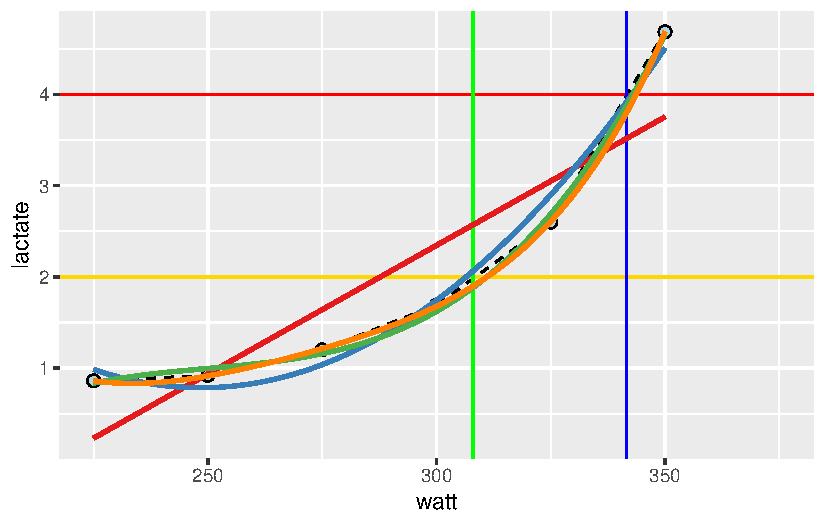
\includegraphics{Oppgave-2_files/figure-pdf/unnamed-chunk-1-1.pdf}

\begin{Shaded}
\begin{Highlighting}[]
\DocumentationTok{\#\#\# vurdering av tilpasningen til de forskjellige lineære modellene på sammenhengen mellom treningsintensitet og laktatakkumulering.}

\NormalTok{lactate }\OtherTok{\textless{}{-}}\NormalTok{ cyclingstudy }\SpecialCharTok{\%\textgreater{}\%}
  \CommentTok{\# utvalg av nødvendige kolonner i analysen.}
  \FunctionTok{select}\NormalTok{(subject, group, timepoint, lac}\FloatTok{.225}\SpecialCharTok{:}\NormalTok{lac}\FloatTok{.375}\NormalTok{) }\SpecialCharTok{\%\textgreater{}\%}
  \CommentTok{\# Kun ein deltaker og ett tidspunkt.}
  \FunctionTok{filter}\NormalTok{(timepoint }\SpecialCharTok{==} \StringTok{"pre"}\NormalTok{, subject }\SpecialCharTok{==} \DecValTok{10}\NormalTok{) }\SpecialCharTok{\%\textgreater{}\%}
  \CommentTok{\# lang format ved å bruke laktatkolonnene.}
  \FunctionTok{pivot\_longer}\NormalTok{(}\AttributeTok{names\_to =} \StringTok{"watt"}\NormalTok{,}
               \AttributeTok{values\_to =} \StringTok{"lactate"}\NormalTok{,}
               \AttributeTok{names\_prefix =} \StringTok{"lac."}\NormalTok{,}
               \AttributeTok{names\_transform =} \FunctionTok{list}\NormalTok{(}\AttributeTok{watt =}\NormalTok{ as.numeric),}
               \AttributeTok{cols =}\NormalTok{ lac}\FloatTok{.225}\SpecialCharTok{:}\NormalTok{lac}\FloatTok{.375}\NormalTok{) }\SpecialCharTok{\%\textgreater{}\%}
  \CommentTok{\# Fjerne dei ugyldige veriene NA for å hindre feilmeldinger.}
  \FunctionTok{filter}\NormalTok{(}\SpecialCharTok{!}\FunctionTok{is.na}\NormalTok{(lactate))}

\CommentTok{\# Legger til en strak linje fra modelen.}
\NormalTok{m1 }\OtherTok{\textless{}{-}} \FunctionTok{lm}\NormalTok{(lactate }\SpecialCharTok{\textasciitilde{}}\NormalTok{ watt, }\AttributeTok{data =}\NormalTok{ lactate)}

\CommentTok{\# Legger til en andregradsplynomisk modell.}
\NormalTok{m2 }\OtherTok{\textless{}{-}} \FunctionTok{lm}\NormalTok{(lactate }\SpecialCharTok{\textasciitilde{}} \FunctionTok{poly}\NormalTok{(watt, }\DecValTok{2}\NormalTok{, }\AttributeTok{raw =} \ConstantTok{TRUE}\NormalTok{), }\AttributeTok{data =}\NormalTok{ lactate)}

\CommentTok{\# Legger til en tredjegradsplynomisk modell.}
\NormalTok{m3 }\OtherTok{\textless{}{-}} \FunctionTok{lm}\NormalTok{(lactate }\SpecialCharTok{\textasciitilde{}} \FunctionTok{poly}\NormalTok{(watt, }\DecValTok{3}\NormalTok{, }\AttributeTok{raw =} \ConstantTok{TRUE}\NormalTok{), }\AttributeTok{data =}\NormalTok{ lactate)}

\CommentTok{\# Legger til en fjerdegradsplynomisk modell.}
\NormalTok{m4 }\OtherTok{\textless{}{-}} \FunctionTok{lm}\NormalTok{(lactate }\SpecialCharTok{\textasciitilde{}} \FunctionTok{poly}\NormalTok{(watt, }\DecValTok{4}\NormalTok{, }\AttributeTok{raw =} \ConstantTok{TRUE}\NormalTok{), }\AttributeTok{data =}\NormalTok{ lactate)}

\CommentTok{\# Lagre alle restverdiene som nye variabler.}
\NormalTok{lactate}\SpecialCharTok{$}\NormalTok{resid.m1 }\OtherTok{\textless{}{-}} \FunctionTok{resid}\NormalTok{(m1)}
\NormalTok{lactate}\SpecialCharTok{$}\NormalTok{resid.m2 }\OtherTok{\textless{}{-}} \FunctionTok{resid}\NormalTok{(m2)}
\NormalTok{lactate}\SpecialCharTok{$}\NormalTok{resid.m3 }\OtherTok{\textless{}{-}} \FunctionTok{resid}\NormalTok{(m3)}
\NormalTok{lactate}\SpecialCharTok{$}\NormalTok{resid.m4 }\OtherTok{\textless{}{-}} \FunctionTok{resid}\NormalTok{(m4)}

\NormalTok{lactate }\SpecialCharTok{\%\textgreater{}\%}
  \CommentTok{\# Samle all data fra modelleme.}
  \FunctionTok{pivot\_longer}\NormalTok{(}\AttributeTok{names\_to =} \StringTok{"model"}\NormalTok{,}
               \AttributeTok{values\_to =} \StringTok{"residual"}\NormalTok{,}
               \AttributeTok{names\_prefix =} \StringTok{"resid."}\NormalTok{,}
               \AttributeTok{names\_transform =} \FunctionTok{list}\NormalTok{(}\AttributeTok{residual =}\NormalTok{ as.numeric),}
               \AttributeTok{cols =}\NormalTok{ resid.m1}\SpecialCharTok{:}\NormalTok{resid.m4) }\SpecialCharTok{\%\textgreater{}\%}
  \CommentTok{\# Plotte verdiene fra den observerte watten på x aksen og restverdiene på y aksen}
  \FunctionTok{ggplot}\NormalTok{(}\FunctionTok{aes}\NormalTok{(watt, residual, }\AttributeTok{fill =}\NormalTok{ model)) }\SpecialCharTok{+} \FunctionTok{geom\_point}\NormalTok{(}\AttributeTok{shape =} \DecValTok{21}\NormalTok{, }\AttributeTok{size =} \DecValTok{3}\NormalTok{) }\SpecialCharTok{+}
  
  \CommentTok{\# For å ha samme farger som over, bruker me scale fill manual.}
  \FunctionTok{scale\_fill\_manual}\NormalTok{(}\AttributeTok{values =} \FunctionTok{c}\NormalTok{(}\StringTok{"\#e41a1c"}\NormalTok{, }\StringTok{"\#377eb8"}\NormalTok{, }\StringTok{"\#4daf4a"}\NormalTok{, }\StringTok{"\#ff7f00"}\NormalTok{))}
\end{Highlighting}
\end{Shaded}

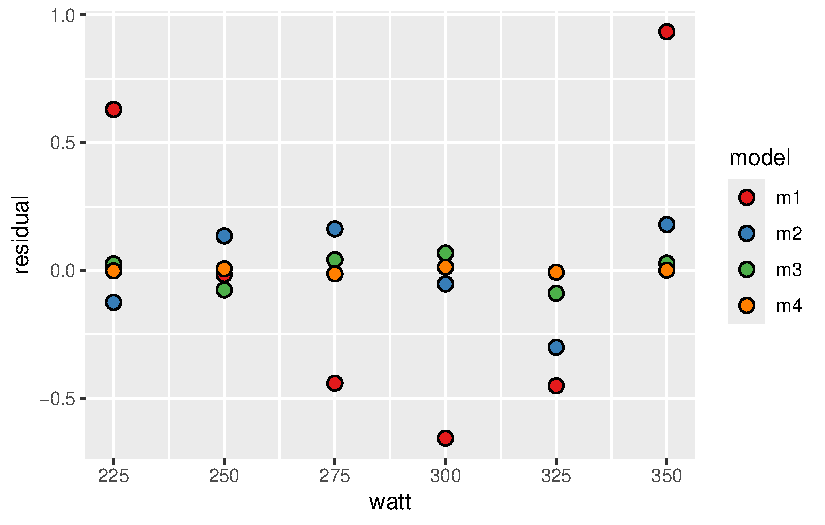
\includegraphics{Oppgave-2_files/figure-pdf/unnamed-chunk-2-1.pdf}

For å finne ut hva forutsatt wattverdi som er nærmest 2 og 4 mmol L-1,
benytter vi koden under:

\begin{Shaded}
\begin{Highlighting}[]
\CommentTok{\# Ny dataramme}
\NormalTok{ndf }\OtherTok{\textless{}{-}} \FunctionTok{data.frame}\NormalTok{(}\AttributeTok{watt =} \FunctionTok{seq}\NormalTok{(}\AttributeTok{from =} \DecValTok{225}\NormalTok{, }\AttributeTok{to =} \DecValTok{350}\NormalTok{, }\AttributeTok{by =} \FloatTok{0.1}\NormalTok{))}

\NormalTok{ndf}\SpecialCharTok{$}\NormalTok{predictions }\OtherTok{\textless{}{-}} \FunctionTok{predict}\NormalTok{(m3, }\AttributeTok{newdata =}\NormalTok{ ndf)}


\CommentTok{\# for å finne ut kva forutsatt Wattverdi som er nermest 2 og 4 mmol L{-}1}
\NormalTok{lactate\_threshold }\OtherTok{\textless{}{-}}\NormalTok{ ndf }\SpecialCharTok{\%\textgreater{}\%}
  \FunctionTok{filter}\NormalTok{(}\FunctionTok{abs}\NormalTok{(predictions }\SpecialCharTok{{-}} \DecValTok{4}\NormalTok{) }\SpecialCharTok{==} \FunctionTok{min}\NormalTok{(}\FunctionTok{abs}\NormalTok{(predictions }\SpecialCharTok{{-}} \DecValTok{4}\NormalTok{)))}

\FunctionTok{summary}\NormalTok{(lactate\_threshold)}
\end{Highlighting}
\end{Shaded}

\begin{verbatim}
      watt      predictions
 Min.   :343   Min.   :4   
 1st Qu.:343   1st Qu.:4   
 Median :343   Median :4   
 Mean   :343   Mean   :4   
 3rd Qu.:343   3rd Qu.:4   
 Max.   :343   Max.   :4   
\end{verbatim}

Her finner vi ut av at på 2 mmol får vi en wattverdi på 311 W, mens på 4
mmol får vi en wattverdi på 343 W. Verdien for 2 mmol ligg på samme
dataframe som kjem fram på 4 mmol L-1.

\section{Del 2: Forutsi størrelser på DNA fragmenter eller stiningene i
en
qPCR-kalibreringskurve}\label{del-2-forutsi-stuxf8rrelser-puxe5-dna-fragmenter-eller-stiningene-i-en-qpcr-kalibreringskurve}

\subsection{Introduksjon}\label{introduksjon-2}

I denne delen av oppgaven tar vi utgangspunkt i forsøket vi gjorde på
molekylærlabben 05. - 06. september, hvor vi ekstraherte DNA fra blod.
Videre forsøkte vi å isolere genene som assosieres med hurtig
muskelfibersammentrekning (R/R) og langsom muskelfibersammentrekning
(X/X) ved hjelp av en PCR-maskin. Prøvene herfra ble testet videre ved
hjelp av elektroforese i agarose gel sammen med en DNA-stige (ladder)
som brukes som markør for å kartlegge genene. Etter elektroforesene tok
vi bilde av preøven slik at vi kunne observere resultatene. Stigen
markerer antall hvert fetiende basebar (bp) opp til 300, og hvert 100.
basepar videre til 1000bp. det dominante R/R-genet har 413bp og det
ressesive X/X-genet har 318bp. De små genmolekylene med få basepar vil
trenge lenger in i gelen under elektroforesen, så X/X-genet vil altså
trenge lenger inn i gelen ved elektroforese. Dette kan være vanskelig å
observere bare med øynene, og vil ikke være særlig nøyaktig. For å få et
mer reliabelt resultat har vi derfor brukt følgende metode. Fra prøvene
våre var det tre brønner som gav resultat - to med et gen, og en med to
(Wackerhage, 2014).

\subsection{Metode}\label{metode-2}

Først har vi brukt ImageJ Fiji for å behandle bildet vi fikk fra
DNA-prøvene. Vi inverterte bildet for å få tydeligere farger, roterte
det rett vei og klipte ut delen av bildet vi ville bruke - altså
analysen av våre prøver. Videre brukte vi rektangelverktøyet for å
markere stigen og prøvene vi ville analysere. Ut fra de markerte
områdene lager ImageJ fiji grafer for hver brønn. Vi markerte
toppunktene i alle grafene som indikerer gen (og trinn på stigen).
Programmet registrerer plasseringen til toppunktene og disse
``koordinatene'' legges inn i et excell-dokument som vi bruker til
beregningene.

\begin{quote}
\begin{quote}
\begin{quote}
\begin{quote}
\begin{quote}
\begin{quote}
\begin{quote}
796d002e0b0ef4c4714dda1e5eb02c80942fb5c8
\end{quote}
\end{quote}
\end{quote}
\end{quote}
\end{quote}
\end{quote}
\end{quote}

\begin{Shaded}
\begin{Highlighting}[]
\FunctionTok{library}\NormalTok{(readxl)}

\NormalTok{dat }\OtherTok{\textless{}{-}} \FunctionTok{read\_excel}\NormalTok{(}\StringTok{"data/resultat\_dna\_analyse.xlsx"}\NormalTok{)}
\end{Highlighting}
\end{Shaded}

For å finne ut av molekylstørrelsen til de ukjente prøvene våre må vi
først kalibrere stigen. Dette gjør vi ved å lage en data.fram som vi
kaller ladder. Her er tallene omvendt proposjonale ettersom det er de
små molekylene som trekkes lengst inn i gelen. Denne dataframen kaller
vi ``ladder''.

Videre må vi også lage en data.fram for de ukjente variablene som vi
kaller ``unknown''

\begin{Shaded}
\begin{Highlighting}[]
\CommentTok{\# lage dataramme for å finne avstand og molekylærvekt}

\NormalTok{ladder }\OtherTok{\textless{}{-}} \FunctionTok{data.frame}\NormalTok{(}\AttributeTok{dist =} \FunctionTok{c}\NormalTok{(}\DecValTok{36}\NormalTok{, }\FloatTok{59.5}\NormalTok{, }\FloatTok{86.5}\NormalTok{,}
                              \FloatTok{119.5}\NormalTok{, }\FloatTok{159.5}\NormalTok{, }\FloatTok{208.5}\NormalTok{,}
                              \FloatTok{269.5}\NormalTok{, }\FloatTok{351.5}\NormalTok{, }\FloatTok{396.5}\NormalTok{,}
                              \FloatTok{455.5}\NormalTok{, }\FloatTok{521.5}\NormalTok{, }\FloatTok{599.5}\NormalTok{, }\FloatTok{701.5}\NormalTok{),}
                     \AttributeTok{mw =} \FunctionTok{c}\NormalTok{(}\DecValTok{1000}\NormalTok{, }\DecValTok{900}\NormalTok{, }\DecValTok{800}\NormalTok{, }
                            \DecValTok{700}\NormalTok{, }\DecValTok{600}\NormalTok{, }\DecValTok{500}\NormalTok{, }
                            \DecValTok{400}\NormalTok{, }\DecValTok{300}\NormalTok{, }\DecValTok{250}\NormalTok{, }
                            \DecValTok{200}\NormalTok{, }\DecValTok{150}\NormalTok{, }\DecValTok{100}\NormalTok{, }\DecValTok{50}\NormalTok{))}

\CommentTok{\# lage ny dataramme med ukjente variabler}

\NormalTok{unknown }\OtherTok{\textless{}{-}} \FunctionTok{data.frame}\NormalTok{(}\AttributeTok{dist =} \FunctionTok{c}\NormalTok{(}\FloatTok{258.5}\NormalTok{, }\FloatTok{262.5}\NormalTok{, }\FloatTok{265.5}\NormalTok{, }\FloatTok{335.5}\NormalTok{))}
\end{Highlighting}
\end{Shaded}

For å lage en kalibreringsmodell bruker vi de samme dataene i ggplot for
å vise stigen. Dette brukes videre for å estimere størrelsen på de
ukjente variablene. Vi valgte å bruke en bøyd graf (poly) for å få minst
mulig avvik.

\begin{Shaded}
\begin{Highlighting}[]
\CommentTok{\# lage en kalibreringsmodell ved hjelp av stigen}

\FunctionTok{library}\NormalTok{(tidyverse)}

\FunctionTok{ggplot}\NormalTok{(}\AttributeTok{data =} \FunctionTok{data.frame}\NormalTok{(}\AttributeTok{x =} \FunctionTok{c}\NormalTok{(}\DecValTok{36}\NormalTok{, }\FloatTok{59.5}\NormalTok{, }\FloatTok{86.5}\NormalTok{,}
                              \FloatTok{119.5}\NormalTok{, }\FloatTok{159.5}\NormalTok{, }\FloatTok{208.5}\NormalTok{,}
                              \FloatTok{269.5}\NormalTok{, }\FloatTok{351.5}\NormalTok{, }\FloatTok{396.5}\NormalTok{,}
                              \FloatTok{455.5}\NormalTok{, }\FloatTok{521.5}\NormalTok{, }\FloatTok{599.5}\NormalTok{, }\FloatTok{701.5}\NormalTok{), }
                         \AttributeTok{y =} \FunctionTok{c}\NormalTok{(}\DecValTok{1000}\NormalTok{, }\DecValTok{900}\NormalTok{, }\DecValTok{800}\NormalTok{, }
                            \DecValTok{700}\NormalTok{, }\DecValTok{600}\NormalTok{, }\DecValTok{500}\NormalTok{, }
                            \DecValTok{400}\NormalTok{, }\DecValTok{300}\NormalTok{, }\DecValTok{250}\NormalTok{, }
                            \DecValTok{200}\NormalTok{, }\DecValTok{150}\NormalTok{, }\DecValTok{100}\NormalTok{, }\DecValTok{50}\NormalTok{)), }
       \FunctionTok{aes}\NormalTok{(x, y)) }\SpecialCharTok{+} \FunctionTok{geom\_point}\NormalTok{() }\SpecialCharTok{+}
  
  \FunctionTok{geom\_smooth}\NormalTok{(}\AttributeTok{method =} \StringTok{"lm"}\NormalTok{, }\AttributeTok{formula =}\NormalTok{ y }\SpecialCharTok{\textasciitilde{}} \FunctionTok{poly}\NormalTok{(x, }\DecValTok{2}\NormalTok{), }
                    \AttributeTok{color =} \StringTok{"green"}\NormalTok{, }\AttributeTok{se =} \ConstantTok{FALSE}\NormalTok{)}\SpecialCharTok{+}
  
  \FunctionTok{scale\_y\_continuous}\NormalTok{(}\AttributeTok{limits =} \FunctionTok{c}\NormalTok{(}\DecValTok{0}\NormalTok{, }\DecValTok{1000}\NormalTok{)) }\SpecialCharTok{+}
  
  \FunctionTok{scale\_x\_continuous}\NormalTok{(}\AttributeTok{limits =} \FunctionTok{c}\NormalTok{(}\DecValTok{0}\NormalTok{, }\DecValTok{750}\NormalTok{))}
\end{Highlighting}
\end{Shaded}

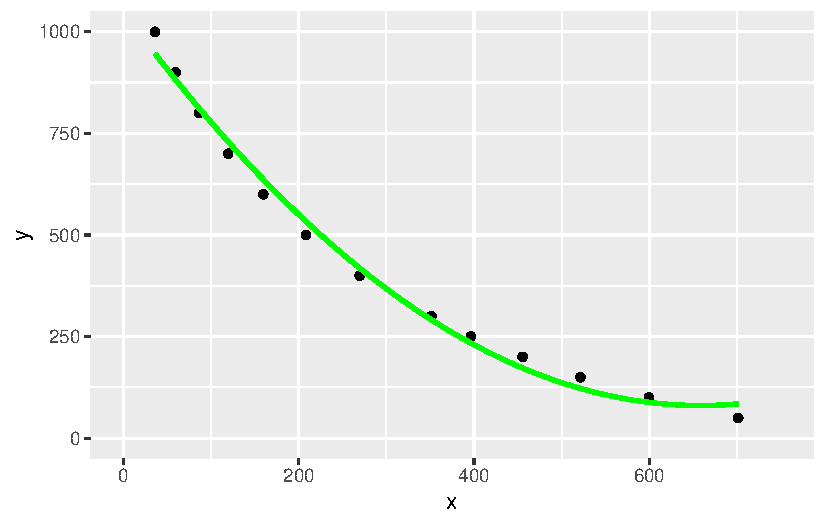
\includegraphics{Oppgave-2_files/figure-pdf/unnamed-chunk-6-1.pdf}

Til slutt brukte vi følgende koder for å estimere molekylstørrelsen på
genene i prøven vår.

\begin{Shaded}
\begin{Highlighting}[]
\CommentTok{\# Fit the model}
\NormalTok{cal }\OtherTok{\textless{}{-}} \FunctionTok{lm}\NormalTok{(}\FunctionTok{log}\NormalTok{(mw) }\SpecialCharTok{\textasciitilde{}}\NormalTok{ dist, }\AttributeTok{data =}\NormalTok{ ladder)}

\CommentTok{\# Check model performance, R\^{}2 should be \textasciitilde{} 1.}
\FunctionTok{summary}\NormalTok{(cal)}
\end{Highlighting}
\end{Shaded}

\begin{verbatim}

Call:
lm(formula = log(mw) ~ dist, data = ladder)

Residuals:
      Min        1Q    Median        3Q       Max 
-0.244363 -0.040218 -0.004565  0.082943  0.112630 

Coefficients:
              Estimate Std. Error t value Pr(>|t|)    
(Intercept)  7.0915695  0.0480419  147.61  < 2e-16 ***
dist        -0.0041842  0.0001298  -32.23 3.06e-12 ***
---
Signif. codes:  0 '***' 0.001 '**' 0.01 '*' 0.05 '.' 0.1 ' ' 1

Residual standard error: 0.09807 on 11 degrees of freedom
Multiple R-squared:  0.9895,    Adjusted R-squared:  0.9886 
F-statistic:  1039 on 1 and 11 DF,  p-value: 3.059e-12
\end{verbatim}

\begin{Shaded}
\begin{Highlighting}[]
\CommentTok{\# Estimate molecular weights from migration distances}
\NormalTok{preds }\OtherTok{\textless{}{-}} \FunctionTok{exp}\NormalTok{(}\FunctionTok{predict}\NormalTok{(cal, }\AttributeTok{newdata =}\NormalTok{ unknown)) }
\end{Highlighting}
\end{Shaded}

Brønn 1: 407 bp Brønn 2: 401 bp Brønn 3: 396 bp og 296 bp

\subsection{Diskusjon}\label{diskusjon}

Denne analysen viser at ingen av genene våre har helt riktig størelse i
forhold til genene vi testet for - R/R (413bp) og X/X (318bp). Vi er
likevel i nærheten som kan tyde på at allelene for brønn 1 og 2 er R/R
og brønn 3 er R/X. Avviket kan forklares med unøyaktighet under
DNA-testen (sansynlig ettersom validitetskontrollen i prøveresultatet
ikke kom fram) og med dårlig kvalitet på bildet som vi brukte i denne
oppgaven. I rapporten fra forsøket tolket vi prøvene annerledes og
trodde at brønn 1, 2 og 3 alle hadde alleler litt over 300bp og at brønn
3 i tillegg hadde en feil med en ukjent allel som var på 250bp. Dette
viser at det er mye unæyaktighet ved å bruke kun øynene til å tolke
resultatet.

\section{Del 3: Tolkning av
regresjonsmodell}\label{del-3-tolkning-av-regresjonsmodell}

\subsection{Introduksjon}\label{introduksjon-3}

I denne delen av oppgaven har vi valgt å se nærmere på variablene
FAST\_NUCLEI\_T1 og TRAINING\_AGE i datasettet \texttt{hypertrofi}, som
er en del av \texttt{exscidata} pakken. For utforming av tabeller,
figurer og grafer bruker vi \texttt{tidyverse}, \texttt{broom} og
\texttt{gt}.

\begin{Shaded}
\begin{Highlighting}[]
\CommentTok{\# Laster inn nødvendige biblioteker}
\FunctionTok{library}\NormalTok{(exscidata)}
\FunctionTok{library}\NormalTok{(tidyverse)}
\FunctionTok{library}\NormalTok{(gt)}
\FunctionTok{library}\NormalTok{(broom)}
\end{Highlighting}
\end{Shaded}

I \texttt{?hypertrofi} er FAST\_NUCLEI\_T1 beskrevet som antall
myonuclei per type-II muskelfiber, mens TRAINING\_AGE viser til antall
år med tidligere treningserfaring. Antall myonuclei per type-II
muskelfiber, kan ha noko å si om muskelens egenskap til å utvikle kraft
og personers styrke (McArdle \emph{et al.}, 2014, kap 22). Det er også
diskutert om trening kan føre til endringer i muskelfiber type eller om
de genetiske faktorene er det som er avgjørende for muskelfiber type
fordelingen til den enkelte (McArdle \emph{et al.}, 2014 p.s.535). Vi
ønsker derfor å se nærmer om det er en lineær sammenheng mellom
FAST\_NUCLEI\_T1 og TRAINING\_AGE i datasettet \texttt{hypertrofi}.

\textbf{Spørsmålet}: Er det et lineært forhold mellom myonuclei per
fiber CSA i type 2 og treningsalder?

\subsection{Metode}\label{metode-3}

Under i Figure~\ref{fig-plot-training-age-myonuclei} er
\texttt{FAST\_NUCLEI\_T1} satt som den avhengige variabelen på y-aksen,
mens \texttt{TRAINING\_AGE} er valgt som den uavhengige variabelen på
x-aksen. Grafen er ment for å gi oss et raskt overblikk av dataene.

\begin{Shaded}
\begin{Highlighting}[]
\CommentTok{\# Laster inn data}
\FunctionTok{data}\NormalTok{(}\StringTok{"hypertrophy"}\NormalTok{)}

\CommentTok{\# Filtrerer ut NA{-}verdier før du velger variabler}
\NormalTok{ds }\OtherTok{\textless{}{-}}\NormalTok{ hypertrophy }\SpecialCharTok{\%\textgreater{}\%}
  \FunctionTok{filter}\NormalTok{(}\SpecialCharTok{!}\FunctionTok{is.na}\NormalTok{(TRAINING\_AGE) }\SpecialCharTok{\&} \SpecialCharTok{!}\FunctionTok{is.na}\NormalTok{(FAST\_NUCLEI\_T1)) }\SpecialCharTok{\%\textgreater{}\%}
  \FunctionTok{select}\NormalTok{(PARTICIPANT, GROUP, TRAINING\_AGE, FAST\_NUCLEI\_T1)}

\CommentTok{\# Plotter data uten NA{-}verdier}
\NormalTok{ds }\SpecialCharTok{\%\textgreater{}\%} 
  \FunctionTok{ggplot}\NormalTok{(}\FunctionTok{aes}\NormalTok{(TRAINING\_AGE, FAST\_NUCLEI\_T1)) }\SpecialCharTok{+}
  \FunctionTok{geom\_point}\NormalTok{(}\AttributeTok{size =} \DecValTok{2}\NormalTok{, }\AttributeTok{fill =} \StringTok{"red"}\NormalTok{) }\SpecialCharTok{+}
  \FunctionTok{geom\_smooth}\NormalTok{(}\AttributeTok{method =} \StringTok{"lm"}\NormalTok{, }\AttributeTok{se =} \ConstantTok{TRUE}\NormalTok{) }\SpecialCharTok{+}
  \FunctionTok{labs}\NormalTok{(}
    \AttributeTok{title =} \StringTok{"Sammenheng mellom treningserfaring og myonuklei"}\NormalTok{,}
    \AttributeTok{x =} \StringTok{"Treningsår"}\NormalTok{, }
    \AttributeTok{y =} \StringTok{"Myonuklei per fiber CSA i Type II"}\NormalTok{) }\SpecialCharTok{+}
  \FunctionTok{theme\_minimal}\NormalTok{()}
\end{Highlighting}
\end{Shaded}

\begin{figure}[H]

\centering{

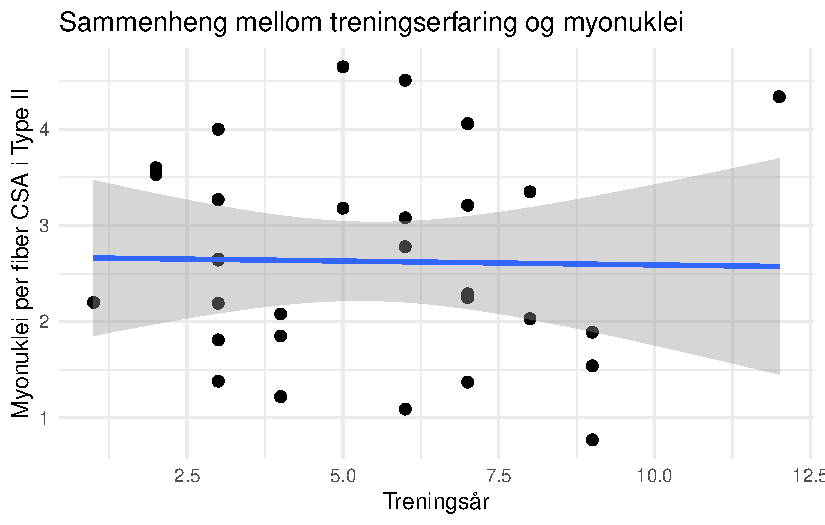
\includegraphics{Oppgave-2_files/figure-pdf/fig-plot-training-age-myonuclei-1.pdf}

}

\caption{\label{fig-plot-training-age-myonuclei}Sammenheng mellom
treningalder og myonuclei per fiber CSA i Type-II}

\end{figure}%

ved hjelp av \texttt{geom\_smooth} har vi lagt inn den best tilpassede
linjen til datapunktene, også kalt lineær regresjonslinje
(Spiegelhalter, 2019\emph{b} p.s.128--129). Det gråe området omkring
regresjonslinjen, visualiserer konfidensintervallet til linjen. Et bredt
konfidensintervall som fremstilt her, indikerer større usikkerhet i
hvordan variablene relaterer til hverandre (Spiegelhalter, 2019\emph{b}
p.s.240--244).

For å presentere regresjonslinjen, har vi laget en lineær statistisk
modell for hjelp til videre tolkning mellom forholdet av dei to
variablene. Oppsummering av de statistiske parametrene som vi har valgt
å fokusere på i diskusjonen vår er listet opp i
Table~\ref{tbl-regresjon} under.

\begin{table}

\caption{\label{tbl-regresjon}Sammenheng mellom treningserfaring og
myonuklei per muskelfiber type-II}

\centering{

\begin{Shaded}
\begin{Highlighting}[]
\CommentTok{\# Lager lineær modell med ds uten NA{-}verdier}
\NormalTok{mod1 }\OtherTok{\textless{}{-}} \FunctionTok{lm}\NormalTok{(FAST\_NUCLEI\_T1 }\SpecialCharTok{\textasciitilde{}}\NormalTok{ TRAINING\_AGE, }\AttributeTok{data =}\NormalTok{ ds)}

\CommentTok{\# Henter ut koeffisienter og deres statistikker}
\NormalTok{model\_summary }\OtherTok{\textless{}{-}} \FunctionTok{tidy}\NormalTok{(mod1)}

\CommentTok{\# Tilpasser p{-}verdier og runder av, og fjerner interceptet}
\NormalTok{model\_summary }\OtherTok{\textless{}{-}}\NormalTok{ model\_summary }\SpecialCharTok{\%\textgreater{}\%}
  \FunctionTok{mutate}\NormalTok{(}
    \AttributeTok{term =} \FunctionTok{ifelse}\NormalTok{(term }\SpecialCharTok{==} \StringTok{"(Intercept)"}\NormalTok{, }\StringTok{"Intercept (Konstantledd)"}\NormalTok{, }\StringTok{"Treningserfaring (år)"}\NormalTok{),}
    \AttributeTok{p.value =} \FunctionTok{ifelse}\NormalTok{(p.value }\SpecialCharTok{\textless{}} \FloatTok{0.001}\NormalTok{, }\StringTok{"\textless{} 0.001"}\NormalTok{, }\FunctionTok{round}\NormalTok{(p.value, }\DecValTok{3}\NormalTok{)),}
    \AttributeTok{estimate =} \FunctionTok{round}\NormalTok{(estimate, }\DecValTok{3}\NormalTok{),}
    \AttributeTok{std.error =} \FunctionTok{round}\NormalTok{(std.error, }\DecValTok{3}\NormalTok{),}
    \AttributeTok{statistic =} \FunctionTok{round}\NormalTok{(statistic, }\DecValTok{3}\NormalTok{)}
\NormalTok{  ) }\SpecialCharTok{\%\textgreater{}\%}
  \CommentTok{\# Filtrer ut interceptet}
  \FunctionTok{filter}\NormalTok{(term }\SpecialCharTok{!=} \StringTok{"Intercept (Konstantledd)"}\NormalTok{)}
  \CommentTok{\# Velger å filtrere ut intercept da det ikkje er aktuelt når vi kun skal se om}
  \CommentTok{\# det er en lineær sammenheng mellom dei to variablene}

\CommentTok{\# Lager regresjonstabell med forklarende radnavn}
\NormalTok{regression\_table }\OtherTok{\textless{}{-}}\NormalTok{ model\_summary }\SpecialCharTok{\%\textgreater{}\%}
  \FunctionTok{select}\NormalTok{(term, estimate, std.error, statistic, p.value) }\SpecialCharTok{\%\textgreater{}\%}
  \FunctionTok{gt}\NormalTok{() }\SpecialCharTok{\%\textgreater{}\%}
  \FunctionTok{fmt\_auto}\NormalTok{() }\SpecialCharTok{\%\textgreater{}\%}
  \FunctionTok{cols\_label}\NormalTok{(}
    \AttributeTok{term =} \StringTok{"Term"}\NormalTok{,}
    \AttributeTok{estimate =} \StringTok{"Estimert koeffisient"}\NormalTok{,}
    \AttributeTok{std.error =} \StringTok{"Standardfeil"}\NormalTok{,}
    \AttributeTok{statistic =} \FunctionTok{md}\NormalTok{(}\StringTok{"*t*{-}verdi"}\NormalTok{),}
    \AttributeTok{p.value =} \FunctionTok{md}\NormalTok{(}\StringTok{"*p*{-}verdi"}\NormalTok{)}
\NormalTok{  ) }\SpecialCharTok{\%\textgreater{}\%}
  \FunctionTok{tab\_source\_note}\NormalTok{(}
    \AttributeTok{source\_note =} \StringTok{"**Notat**: *p*{-}verdier mindre enn 0.05 anses som statistisk signifikante."}
\NormalTok{  )}

\CommentTok{\# Vis resultatene}
\FunctionTok{print}\NormalTok{(regression\_table)}
\end{Highlighting}
\end{Shaded}

\phantomsection\label{svpqugopfc}
Term

Estimert koeffisient

Standardfeil

{{t-verdi}}

{{p-verdi}}

Treningserfaring (år)

−0.008

0.077

−0.104

0.918

\textbf{Notat}: \emph{p}-verdier mindre enn 0.05 anses som statistisk
signifikante.

}

\end{table}%

\subsection{Diskusjon}\label{diskusjon-1}

I tabellen kan vi lese av verdiene for estimert koeffisient
(regresjonskoeffisient), standardfeil, t-verdi og p-verdi. Den estimerte
koeffisenten til ``Treningserfaring (år)'' forteller oss hvor mye
\texttt{FAST\_NUCLEI\_T1} endres per enhet økning i
\texttt{TRAINING\_AGE}. I vårt tilfelle ser man en antall nukleikjerner
per fiber reduseres med 0.008 per år med treningserfaring.

Standardfeilen måler hvor mye koeffisientene er forventet å variere fra
utvalg til utvalg. Standardfeilen som vi har fått er liten i tallverdi,
og man kan da fort konkludere at estimeringen er presis grunnet lav
standardfeil. Samtidig er det viktig å se standardfeilen i lys av den
estimerte koefisienten. I forhold til koeffisienten selv, er
standardfeilen stor, og betyr at man burde være usikker på nøyaktigheten
til estimatet (Spiegelhalter, 2019\emph{b} p.s.230--232)

\emph{t-verdien} sier hvor mange standardavvik den estimerte
koeffisienten er fra 0, der jo høyere t-verdien (enten negativ eller
positiv), dess mer signifikant er koeffisienten (Spiegelhalter,
2019\emph{b} p.s.275--276). Hos oss er t-verdien -0.104, noe som
indikerer at det ikke er noe signifikant lineær sammenheng mellom
\texttt{FAST\_NUCLEI\_T1} og \texttt{TRAINING\_AGE}.

Nært knyttet til t-verdien, har man \emph{p-verdien} som hjelper oss å
si om t-verdien er statistisk signifikant. P-verdi er sannsynligheten
for å observere en så ekstrem teststatistikk som den t-verdien vi har
fått, gitt antagelsen at det ikke er en sammenheng mellom variablene
våre (Spiegelhalter, 2019\emph{b} p.s.264--265). Basert på at p-verdien
i vår modell er 0.918, er det 91,8 \% sannsynlighet at man vil observere
en t-verdi på -0.008. Vi har derfor ikkje tilstrekkelig bevis for å
kunne si at den uavhengige variabelen \texttt{TRAINING\_AGE} har en
effekt på den avhengige variabelen \texttt{FAST\_NUCLEI\_T1}, og at det
er en statistik lineær sammenheng mellom variablene (Spiegelhalter,
2019\emph{b} p.s.265--268).

Selv om p-verdi er et nyttig verktøy for å hjelpe oss å trekke
slutninger om koeffisientenes statistiske signifikans, sier den oss ikke
noe om størrelsen på en effekt eller hva praktisk betydning den kan ha.
Størrelsen på datasettet har også en betydning på p-verdien, der små
datasett, som det vi har, kan gi høye p-verdier selv om det er en
betydelig effekt (Spiegelhalter, 2019\emph{b} p.s.285)

\bookmarksetup{startatroot}

\chapter{Slutninger fra statistiske modeller og statistisk
styrke}\label{slutninger-fra-statistiske-modeller-og-statistisk-styrke}

\section{Introduksjon}\label{introduksjon-4}

I denne oppgaven skal se på statistisk forskning. Vi skal simulere to
forskningsprosjekt med forskjellig størrelse på utvalg. Den første
gruppen (m1) har et utvalg på 8 målinger, og den andre gruppen har et
utvalg på 40 målinger. Vi skal se hva forskjellig størrelse på utvalg
gjør med resultatene.

\section{Simulasjon}\label{simulasjon}

\begin{Shaded}
\begin{Highlighting}[]
\FunctionTok{library}\NormalTok{(tidyverse)}

\FunctionTok{set.seed}\NormalTok{(}\DecValTok{1}\NormalTok{)}
\NormalTok{population }\OtherTok{\textless{}{-}} \FunctionTok{rnorm}\NormalTok{(}\DecValTok{1000000}\NormalTok{, }\AttributeTok{mean =} \FloatTok{1.5}\NormalTok{, }\AttributeTok{sd =} \DecValTok{3}\NormalTok{)}


\NormalTok{samp1 }\OtherTok{\textless{}{-}} \FunctionTok{data.frame}\NormalTok{(}\AttributeTok{y =} \FunctionTok{sample}\NormalTok{(population, }\DecValTok{8}\NormalTok{, }\AttributeTok{replace =} \ConstantTok{FALSE}\NormalTok{))}

\NormalTok{samp2 }\OtherTok{\textless{}{-}} \FunctionTok{data.frame}\NormalTok{(}\AttributeTok{y =} \FunctionTok{sample}\NormalTok{(population, }\DecValTok{40}\NormalTok{, }\AttributeTok{replace =} \ConstantTok{FALSE}\NormalTok{))}


\NormalTok{m1 }\OtherTok{\textless{}{-}} \FunctionTok{lm}\NormalTok{(y }\SpecialCharTok{\textasciitilde{}} \DecValTok{1}\NormalTok{, }\AttributeTok{data =}\NormalTok{ samp1)}
\NormalTok{m2 }\OtherTok{\textless{}{-}} \FunctionTok{lm}\NormalTok{(y }\SpecialCharTok{\textasciitilde{}} \DecValTok{1}\NormalTok{, }\AttributeTok{data =}\NormalTok{ samp2)}

\FunctionTok{summary}\NormalTok{(m1)}
\end{Highlighting}
\end{Shaded}

\begin{verbatim}

Call:
lm(formula = y ~ 1, data = samp1)

Residuals:
    Min      1Q  Median      3Q     Max 
-6.5322 -1.2523 -0.0883  1.3540  4.8692 

Coefficients:
            Estimate Std. Error t value Pr(>|t|)
(Intercept)    1.840      1.251    1.47    0.185

Residual standard error: 3.539 on 7 degrees of freedom
\end{verbatim}

\begin{Shaded}
\begin{Highlighting}[]
\FunctionTok{summary}\NormalTok{(m2)}
\end{Highlighting}
\end{Shaded}

\begin{verbatim}

Call:
lm(formula = y ~ 1, data = samp2)

Residuals:
    Min      1Q  Median      3Q     Max 
-5.6557 -2.2883  0.2636  2.2549  6.4212 

Coefficients:
            Estimate Std. Error t value Pr(>|t|)   
(Intercept)   1.5642     0.4774   3.276  0.00221 **
---
Signif. codes:  0 '***' 0.001 '**' 0.01 '*' 0.05 '.' 0.1 ' ' 1

Residual standard error: 3.019 on 39 degrees of freedom
\end{verbatim}

\subsection{Oppgave 1.}\label{oppgave-1.}

\textbf{Explain the estimate, SE, t-value, and p-value from the
regression models that we created previously (m1 and m2).}

Over kan vi se resultatene av simuleringen. og vi får følgende
resultater:

\begin{longtable}[]{@{}lll@{}}
\toprule\noalign{}
& m1 & m2 \\
\midrule\noalign{}
\endhead
\bottomrule\noalign{}
\endlastfoot
Estimat & 1.84 & 1.5642 \\
Standard feil & 1.251 & 0.4774 \\
t-verdi & 1.47 & 3.276 \\
p-verdi & 0.185 & 0.00221 \\
\end{longtable}

\subsection{Oppgave 2.}\label{oppgave-2.}

\textbf{Discuss what contributes to the different results in the two
studies (m1 and m2).}

Når vi øker størelsen på utvalget ser vi at dette påvirker resultatene.
I en faktisk forskning vil vi jo ikke vite det faktiske gjennomsnittet i
en populasjon. I denne simuleringen derimot har vi bestemt at
gjennomsnittet (mean) er 1.5. Når vi har et utvalg på 8 observasjoner
får vi resultatet 1.84, og med 40 observasjoner får vi 1.56 som estimat.
Ved å øke antall faktiske observasjoner kan vi altså gjøre et mer
presist estimat av hva som er gjennomsnittet i en populasjon.

På samme måte vil størelsen på utvalget påvirke standard feilen i
forsøket. Standard feil beregnes ved å dele standard avvik, som i denne
simuleringen er 3 på kvadratroten av antall observasjoner. I denne
simuleringen blir det altså tre delt på kvadratroten av 8 i m1, og
kvadratroten av 40 i m2. Som vi kan se får vi da lavere standers feil i
m2 hvor utvalget er større. Standard feil handler nemlig om hvor
sannsynlig det er at utvalger er representativt for populasjonene. Lav
standard feil betyr at det er stor sansynlighet for at utvalget er
representativt.

T-verdien beregnes ved å dele estimatet med standard feil og forteller
oss om forskjellen i gruppene er signifikant (Spiegelhalter,
2019\emph{a}). Videre sier Spieghalter at en t-verdi over 2 tilsvarer en
p-verdi, som er et mål på forskjellen mellom innsamlet data og
null-hypotesen, under 0,05 som igjen vil bety at statisitkken er
signifikant. I vår simulering kan vi se at dette blir avgjørende. I
simuleringen med 8 i utvalger får vi en t-verdi på 1.47 som tilsvarer en
p-verdi på 0.185 altså ikke signifikant. I utvalget med 40 derimot er
t-verdien 3,276 og p-verdien 0.00221 som vil si at resultatet er
signifikant. I forsøket med 8 observasjoner ville det altså ha blitt
gjort en type II feil, altså a avvise en korrekt alternativ hypotese
fordi testresultatet støtter null-hypotesen (Spiegelhalter,
2019\emph{a}).

\subsection{Oppgave 3.}\label{oppgave-3.}

\textbf{Why do we use the shaded area in the lower and upper tail of the
t-distribution (See Figure).}

Grafen viser en tosidig p-verdi for m1. Midt i grafen ser vi det
estimerte gjennomsnittet. En tosidig p-verdi sier noe om hvor mange
observasjoner vi kan regne med å få fra populasjonen som er like
ekstreme eller mer ekstreme enn den observerte t-verdien (Spiegelhalter,
2019\emph{a}). De blå feltene viser altså hvor mange observasjoner vi
kan ha utenfor null-hypotesen uten at null-hypotesen blir motbevist.

\section{Many studies}\label{many-studies}

\begin{Shaded}
\begin{Highlighting}[]
\FunctionTok{library}\NormalTok{(tidyverse)}

\FunctionTok{set.seed}\NormalTok{(}\DecValTok{1}\NormalTok{)}
\NormalTok{population }\OtherTok{\textless{}{-}} \FunctionTok{rnorm}\NormalTok{(}\DecValTok{1000000}\NormalTok{, }\AttributeTok{mean =} \FloatTok{1.5}\NormalTok{, }\AttributeTok{sd =} \DecValTok{3}\NormalTok{)}

\CommentTok{\# Create data frames to store the model estimates}
\NormalTok{results\_8 }\OtherTok{\textless{}{-}} \FunctionTok{data.frame}\NormalTok{(}\AttributeTok{estimate =} \FunctionTok{rep}\NormalTok{(}\ConstantTok{NA}\NormalTok{, }\DecValTok{1000}\NormalTok{), }
                      \AttributeTok{se =} \FunctionTok{rep}\NormalTok{(}\ConstantTok{NA}\NormalTok{, }\DecValTok{1000}\NormalTok{), }
                      \AttributeTok{pval =} \FunctionTok{rep}\NormalTok{(}\ConstantTok{NA}\NormalTok{, }\DecValTok{1000}\NormalTok{), }
                      \AttributeTok{n =} \DecValTok{8}\NormalTok{)  }

\NormalTok{results\_40 }\OtherTok{\textless{}{-}} \FunctionTok{data.frame}\NormalTok{(}\AttributeTok{estimate =} \FunctionTok{rep}\NormalTok{(}\ConstantTok{NA}\NormalTok{, }\DecValTok{1000}\NormalTok{), }
                      \AttributeTok{se =} \FunctionTok{rep}\NormalTok{(}\ConstantTok{NA}\NormalTok{, }\DecValTok{1000}\NormalTok{), }
                      \AttributeTok{pval =} \FunctionTok{rep}\NormalTok{(}\ConstantTok{NA}\NormalTok{, }\DecValTok{1000}\NormalTok{), }
                      \AttributeTok{n =} \DecValTok{40}\NormalTok{)}

\CommentTok{\# A for loop used to sample 1000 studies, each iteration (i) will draw a new sample}
\CommentTok{\# from the population. }

\ControlFlowTok{for}\NormalTok{(i }\ControlFlowTok{in} \DecValTok{1}\SpecialCharTok{:}\DecValTok{1000}\NormalTok{) \{}
  
  \CommentTok{\# Draw a sample }
\NormalTok{  samp1 }\OtherTok{\textless{}{-}} \FunctionTok{data.frame}\NormalTok{(}\AttributeTok{y =} \FunctionTok{sample}\NormalTok{(population, }\DecValTok{8}\NormalTok{, }\AttributeTok{replace =} \ConstantTok{FALSE}\NormalTok{))}
\NormalTok{  samp2 }\OtherTok{\textless{}{-}} \FunctionTok{data.frame}\NormalTok{(}\AttributeTok{y =} \FunctionTok{sample}\NormalTok{(population, }\DecValTok{40}\NormalTok{, }\AttributeTok{replace =} \ConstantTok{FALSE}\NormalTok{))}

  \CommentTok{\# Model the data}
\NormalTok{  m1 }\OtherTok{\textless{}{-}} \FunctionTok{lm}\NormalTok{(y }\SpecialCharTok{\textasciitilde{}} \DecValTok{1}\NormalTok{, }\AttributeTok{data =}\NormalTok{ samp1)}
\NormalTok{  m2 }\OtherTok{\textless{}{-}} \FunctionTok{lm}\NormalTok{(y }\SpecialCharTok{\textasciitilde{}} \DecValTok{1}\NormalTok{, }\AttributeTok{data =}\NormalTok{ samp2)}
  
  \CommentTok{\# Extract values from the models}
\NormalTok{  results\_8[i, }\DecValTok{1}\NormalTok{] }\OtherTok{\textless{}{-}} \FunctionTok{coef}\NormalTok{(}\FunctionTok{summary}\NormalTok{(m1))[}\DecValTok{1}\NormalTok{, }\DecValTok{1}\NormalTok{]}
\NormalTok{  results\_8[i, }\DecValTok{2}\NormalTok{] }\OtherTok{\textless{}{-}} \FunctionTok{coef}\NormalTok{(}\FunctionTok{summary}\NormalTok{(m1))[}\DecValTok{1}\NormalTok{, }\DecValTok{2}\NormalTok{]}
\NormalTok{  results\_8[i, }\DecValTok{3}\NormalTok{] }\OtherTok{\textless{}{-}} \FunctionTok{coef}\NormalTok{(}\FunctionTok{summary}\NormalTok{(m1))[}\DecValTok{1}\NormalTok{, }\DecValTok{4}\NormalTok{]}

\NormalTok{  results\_40[i, }\DecValTok{1}\NormalTok{] }\OtherTok{\textless{}{-}} \FunctionTok{coef}\NormalTok{(}\FunctionTok{summary}\NormalTok{(m2))[}\DecValTok{1}\NormalTok{, }\DecValTok{1}\NormalTok{]}
\NormalTok{  results\_40[i, }\DecValTok{2}\NormalTok{] }\OtherTok{\textless{}{-}} \FunctionTok{coef}\NormalTok{(}\FunctionTok{summary}\NormalTok{(m2))[}\DecValTok{1}\NormalTok{, }\DecValTok{2}\NormalTok{]}
\NormalTok{  results\_40[i, }\DecValTok{3}\NormalTok{] }\OtherTok{\textless{}{-}} \FunctionTok{coef}\NormalTok{(}\FunctionTok{summary}\NormalTok{(m2))[}\DecValTok{1}\NormalTok{, }\DecValTok{4}\NormalTok{]}
  
  
\NormalTok{\}}


\CommentTok{\# Save the results in a combined data frame}

\NormalTok{results }\OtherTok{\textless{}{-}} \FunctionTok{bind\_rows}\NormalTok{(results\_8, results\_40)}
\end{Highlighting}
\end{Shaded}

\subsection{Oppgave 4.}\label{oppgave-4.}

\textbf{Calculate the standard deviation of the estimate variable, and
the average of the se variable for each of the study sample sizes (8 and
40). Explain why these numbers are very similar. How can you define the
Standard Error (SE) in light of these calculations?}

m1: 8

\begin{Shaded}
\begin{Highlighting}[]
\FunctionTok{library}\NormalTok{(dplyr)}

\CommentTok{\# Beregn standardavviket til estimate og gjennomsnittet av se for hver utvalgsstørrelse}
\NormalTok{results\_summary }\OtherTok{\textless{}{-}}\NormalTok{ results }\SpecialCharTok{\%\textgreater{}\%}
  \FunctionTok{group\_by}\NormalTok{(n) }\SpecialCharTok{\%\textgreater{}\%}
  \FunctionTok{summarise}\NormalTok{(}
    \AttributeTok{mean =} \FunctionTok{mean}\NormalTok{(estimate),}
    \AttributeTok{std\_estimate =} \FunctionTok{sd}\NormalTok{(estimate),  }\CommentTok{\# Standardavviket til estimate}
    \AttributeTok{avg\_se =} \FunctionTok{mean}\NormalTok{(se)             }\CommentTok{\# Gjennomsnittet av standardfeilen}
\NormalTok{  )}

\CommentTok{\# Vis sammendraget av resultatene}
\FunctionTok{print}\NormalTok{(results\_summary)}
\end{Highlighting}
\end{Shaded}

\begin{verbatim}
# A tibble: 2 x 4
      n  mean std_estimate avg_se
  <dbl> <dbl>        <dbl>  <dbl>
1     8  1.52        1.07   1.02 
2    40  1.51        0.484  0.470
\end{verbatim}

Som vi kan se over er standard avvik og gjennomsnitlig standard feil
svært like. Forskjellen er 0,05 i m1 og 0,014 i m2. Grunnen til at
standard avvik og standard feil er så like er på grunn av de henger
sammen. Standard feil finner vi som tidligere nevn ved å dele standard
avvik på kvadratroten av utvalget. Begge disse verdiene blir brukt for å
lage kurvemodeller som viser p-verdi og t-verdi. Når vi får lavere
standard avvik og standard feil vil kurven bli smalere og spissere,
fordi estimatet kommer nærmere det faktiske gjennomsnittet. hvis vi
skulle laget en kurve ut fra utvalgene m1 og m2, ville altså m1 være
bredere og rundere enn m2 som ville være smal og spiss.

beregne kurven

\subsection{Oppgave 5.}\label{oppgave-5.}

\textbf{Create a histogram (see example code below) of the p-values from
each study sample-size. How do you interpret these histograms, what do
they tell you about the effect of sample size on statistical power?}

\begin{Shaded}
\begin{Highlighting}[]
\CommentTok{\# Example code for copy and paste}

\CommentTok{\# A two facets histogram can be created with ggplot2}
\NormalTok{results }\SpecialCharTok{\%\textgreater{}\%}
  \FunctionTok{ggplot}\NormalTok{(}\FunctionTok{aes}\NormalTok{(pval)) }\SpecialCharTok{+} 
  \FunctionTok{geom\_histogram}\NormalTok{() }\SpecialCharTok{+}
  \FunctionTok{facet\_wrap}\NormalTok{(}\SpecialCharTok{\textasciitilde{}}\NormalTok{ n)}
\end{Highlighting}
\end{Shaded}

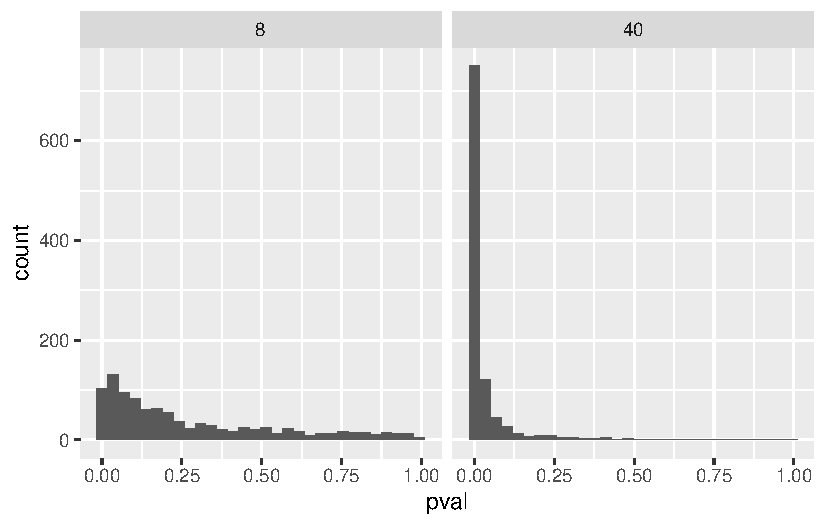
\includegraphics{Oppgave-3_files/figure-pdf/unnamed-chunk-4-1.pdf}

I denne oppgaven kan vi se hva jeg snakket om i forrige oppgave. Et
større utvalg vil gjøre at histogrammet blir smalere og spissere. Vi
samler estimatene mot gjennomsnittet. Som vi kan se fra histogrammene
vil et større utvalg gi lavere p-verdi, som i dette tilfelle vil gjøre
resultatet signifikant som jeg har vist tidligere i oppgaven. Statistisk
styrke er sansynligheten for å korrekt forkaste nullhypotesen gitt at
den nye hypotesen stemmer, har en klar sammenheng med utvalgstørrelsen
(Spiegelhalter, 2019\emph{a}). Med større utvalg vil altså styrken øke,
som vi også kan se i utregningen over.

\subsection{Oppgave 6.}\label{oppgave-6.}

\textbf{Calculate the number of studies from each sample size that
declare a statistical significant effect (specify a threshold for, your
significance level).}

\begin{Shaded}
\begin{Highlighting}[]
\CommentTok{\# Count the proportion of tests below a certain p{-}value for each }
\NormalTok{results }\SpecialCharTok{\%\textgreater{}\%}
  \FunctionTok{filter}\NormalTok{(pval }\SpecialCharTok{\textless{}} \FloatTok{0.05}\NormalTok{) }\SpecialCharTok{\%\textgreater{}\%}
  \FunctionTok{group\_by}\NormalTok{(n) }\SpecialCharTok{\%\textgreater{}\%}
  \FunctionTok{summarise}\NormalTok{(}\AttributeTok{sig\_results =} \FunctionTok{n}\NormalTok{()}\SpecialCharTok{/}\DecValTok{1000}\NormalTok{)}
\end{Highlighting}
\end{Shaded}

\begin{verbatim}
# A tibble: 2 x 2
      n sig_results
  <dbl>       <dbl>
1     8       0.227
2    40       0.865
\end{verbatim}

I denne beregningen skal jeg finne ut hvor mange studier med
utvalgsstørelser 8 (lik m1) og 40 (lik m2) som vil få statistisk
signifikante resultat med en p-verdi \textless{} 0,05. Her får jeg
resultatene 0,227 for m1, og 0,865 for m2. Dette kan vi gjøre om til
prosentverier: m1: 22,7 \% og m2: 86,5 \%. Det er altså stor forskjell
på den betydelige effekten på de forskjellige studiene. I studier med 8
deltakere vil det bare vaære 22,7 \% sjanse for a få et statistisk
sikgnifikant resultat, mens det i studier med 40 vil være 86,5 \% sjanse
for å få et statistisk signifikant resultat.

\subsection{Oppgave 7.}\label{oppgave-7.}

\textbf{Using the pwr package, calculate the power of a one-sample
t-test, with a effect size of 1.5/3, your specified significance level
and sample sizes 8 and 40. Explain the results in the light of your
simulations.}

\begin{Shaded}
\begin{Highlighting}[]
\CommentTok{\# Using the pwr package}
\FunctionTok{library}\NormalTok{(pwr)}

\FunctionTok{pwr.t.test}\NormalTok{(}\AttributeTok{n =} \DecValTok{8}\NormalTok{, }\AttributeTok{sig.level =} \FloatTok{0.05}\NormalTok{, }\AttributeTok{d =} \FloatTok{1.5}\SpecialCharTok{/}\DecValTok{3}\NormalTok{, }\AttributeTok{type =} \StringTok{"one.sample"}\NormalTok{)}
\end{Highlighting}
\end{Shaded}

\begin{verbatim}

     One-sample t test power calculation 

              n = 8
              d = 0.5
      sig.level = 0.05
          power = 0.232077
    alternative = two.sided
\end{verbatim}

\begin{Shaded}
\begin{Highlighting}[]
\FunctionTok{pwr.t.test}\NormalTok{(}\AttributeTok{n =} \DecValTok{40}\NormalTok{, }\AttributeTok{sig.level =} \FloatTok{0.05}\NormalTok{, }\AttributeTok{d =} \FloatTok{1.5}\SpecialCharTok{/}\DecValTok{3}\NormalTok{, }\AttributeTok{type =} \StringTok{"one.sample"}\NormalTok{)}
\end{Highlighting}
\end{Shaded}

\begin{verbatim}

     One-sample t test power calculation 

              n = 40
              d = 0.5
      sig.level = 0.05
          power = 0.8693981
    alternative = two.sided
\end{verbatim}

Statistisk styrke er sannsynligheten for å korrekt avvise
null-hypotesen, gitt at den alternative hypotesen er sann
(Spiegelhalter, 2019\emph{a}). Lav statistisk styrke øker
sannsynligheten for å begå type I feil som vil si at man feilaktiv
avviser en korrekt null-hypotese (Spiegelhalter, 2019\emph{a}). Her får
m1 en statistisk styrke på 0,232. Dette stemmer bra med simuleringen i
oppgave 6. I m2 derimot får vi en statistisk styrke på 0,869 som er en
ganske høy statistisk styrke. I studien m2 er det altså lav
sannsynlighet for å begå en type I feil. Dette støtter igjen det jeg har
kommet fram til i tidligere oppgaver om at større utvalg øker
sannsynligheten for et korrekt resultat, og at hvis vi skulle stole på
resultatene fra m1 ville vi begå en type II feil.

\section{Many studies without population
effect}\label{many-studies-without-population-effect}

\subsection{Oppgave 8.}\label{oppgave-8.}

\textbf{With a significance level of 5\%, how many studies would give
you a ``false positive'' result if you did many repeated studies?}

\begin{Shaded}
\begin{Highlighting}[]
\NormalTok{population }\OtherTok{\textless{}{-}} \FunctionTok{rnorm}\NormalTok{(}\DecValTok{1000000}\NormalTok{, }\AttributeTok{mean =} \DecValTok{0}\NormalTok{, }\AttributeTok{sd =} \DecValTok{3}\NormalTok{)}


\CommentTok{\# Create data frames to store the model estimates}
\NormalTok{results\_8 }\OtherTok{\textless{}{-}} \FunctionTok{data.frame}\NormalTok{(}\AttributeTok{estimate =} \FunctionTok{rep}\NormalTok{(}\ConstantTok{NA}\NormalTok{, }\DecValTok{1000}\NormalTok{), }
                      \AttributeTok{se =} \FunctionTok{rep}\NormalTok{(}\ConstantTok{NA}\NormalTok{, }\DecValTok{1000}\NormalTok{), }
                      \AttributeTok{pval =} \FunctionTok{rep}\NormalTok{(}\ConstantTok{NA}\NormalTok{, }\DecValTok{1000}\NormalTok{), }
                      \AttributeTok{n =} \DecValTok{8}\NormalTok{)  }

\NormalTok{results\_40 }\OtherTok{\textless{}{-}} \FunctionTok{data.frame}\NormalTok{(}\AttributeTok{estimate =} \FunctionTok{rep}\NormalTok{(}\ConstantTok{NA}\NormalTok{, }\DecValTok{1000}\NormalTok{), }
                      \AttributeTok{se =} \FunctionTok{rep}\NormalTok{(}\ConstantTok{NA}\NormalTok{, }\DecValTok{1000}\NormalTok{), }
                      \AttributeTok{pval =} \FunctionTok{rep}\NormalTok{(}\ConstantTok{NA}\NormalTok{, }\DecValTok{1000}\NormalTok{), }
                      \AttributeTok{n =} \DecValTok{40}\NormalTok{)}

\CommentTok{\# A for loop used to sample 1000 studies, each iteration (i) will draw a new sample}
\CommentTok{\# from the population. }

\ControlFlowTok{for}\NormalTok{(i }\ControlFlowTok{in} \DecValTok{1}\SpecialCharTok{:}\DecValTok{1000}\NormalTok{) \{}
  
  \CommentTok{\# Draw a sample }
\NormalTok{  samp1 }\OtherTok{\textless{}{-}} \FunctionTok{data.frame}\NormalTok{(}\AttributeTok{y =} \FunctionTok{sample}\NormalTok{(population, }\DecValTok{8}\NormalTok{, }\AttributeTok{replace =} \ConstantTok{FALSE}\NormalTok{))}
\NormalTok{  samp2 }\OtherTok{\textless{}{-}} \FunctionTok{data.frame}\NormalTok{(}\AttributeTok{y =} \FunctionTok{sample}\NormalTok{(population, }\DecValTok{40}\NormalTok{, }\AttributeTok{replace =} \ConstantTok{FALSE}\NormalTok{))}

  \CommentTok{\# Model the data}
\NormalTok{  m1 }\OtherTok{\textless{}{-}} \FunctionTok{lm}\NormalTok{(y }\SpecialCharTok{\textasciitilde{}} \DecValTok{1}\NormalTok{, }\AttributeTok{data =}\NormalTok{ samp1)}
\NormalTok{  m2 }\OtherTok{\textless{}{-}} \FunctionTok{lm}\NormalTok{(y }\SpecialCharTok{\textasciitilde{}} \DecValTok{1}\NormalTok{, }\AttributeTok{data =}\NormalTok{ samp2)}
  
  \CommentTok{\# Extract values from the models}
\NormalTok{  results\_8[i, }\DecValTok{1}\NormalTok{] }\OtherTok{\textless{}{-}} \FunctionTok{coef}\NormalTok{(}\FunctionTok{summary}\NormalTok{(m1))[}\DecValTok{1}\NormalTok{, }\DecValTok{1}\NormalTok{]}
\NormalTok{  results\_8[i, }\DecValTok{2}\NormalTok{] }\OtherTok{\textless{}{-}} \FunctionTok{coef}\NormalTok{(}\FunctionTok{summary}\NormalTok{(m1))[}\DecValTok{1}\NormalTok{, }\DecValTok{2}\NormalTok{]}
\NormalTok{  results\_8[i, }\DecValTok{3}\NormalTok{] }\OtherTok{\textless{}{-}} \FunctionTok{coef}\NormalTok{(}\FunctionTok{summary}\NormalTok{(m1))[}\DecValTok{1}\NormalTok{, }\DecValTok{4}\NormalTok{]}

\NormalTok{  results\_40[i, }\DecValTok{1}\NormalTok{] }\OtherTok{\textless{}{-}} \FunctionTok{coef}\NormalTok{(}\FunctionTok{summary}\NormalTok{(m2))[}\DecValTok{1}\NormalTok{, }\DecValTok{1}\NormalTok{]}
\NormalTok{  results\_40[i, }\DecValTok{2}\NormalTok{] }\OtherTok{\textless{}{-}} \FunctionTok{coef}\NormalTok{(}\FunctionTok{summary}\NormalTok{(m2))[}\DecValTok{1}\NormalTok{, }\DecValTok{2}\NormalTok{]}
\NormalTok{  results\_40[i, }\DecValTok{3}\NormalTok{] }\OtherTok{\textless{}{-}} \FunctionTok{coef}\NormalTok{(}\FunctionTok{summary}\NormalTok{(m2))[}\DecValTok{1}\NormalTok{, }\DecValTok{4}\NormalTok{]}
  
  
\NormalTok{\}}


\CommentTok{\# Save the results in a combined data frame}

\NormalTok{results\_null }\OtherTok{\textless{}{-}} \FunctionTok{bind\_rows}\NormalTok{(results\_8, results\_40)}
\end{Highlighting}
\end{Shaded}

\begin{Shaded}
\begin{Highlighting}[]
\CommentTok{\# Calculate number of false positives}

\NormalTok{false\_positives }\OtherTok{\textless{}{-}}\NormalTok{ results\_null }\SpecialCharTok{\%\textgreater{}\%}
  \FunctionTok{filter}\NormalTok{(pval }\SpecialCharTok{\textless{}} \FloatTok{0.05}\NormalTok{) }\SpecialCharTok{\%\textgreater{}\%}
  \FunctionTok{group\_by}\NormalTok{(n) }\SpecialCharTok{\%\textgreater{}\%}
  \FunctionTok{summarise}\NormalTok{(}\AttributeTok{sig\_results =} \FunctionTok{n}\NormalTok{() }\SpecialCharTok{/} \DecValTok{1000}\NormalTok{)}

\CommentTok{\# Print results}
\FunctionTok{print}\NormalTok{(false\_positives)}
\end{Highlighting}
\end{Shaded}

\begin{verbatim}
# A tibble: 2 x 2
      n sig_results
  <dbl>       <dbl>
1     8       0.053
2    40       0.053
\end{verbatim}

Fra resultatene o simuleringen over kan vi se at vi får det samme
resultatet for begge utvalgstørrelsene, nemlig 0,053. Dette vil si at
ved å gjennomføre forsøkene gjenntatte ganger i den samme populasjonen
vil 5,3 \% av forsøkene gi falsk positivt resultat. Dette virker ved
første øyenkast rart fordi et større utvalg skal i utgangspunkte
redusere sjansen for å få falsk positivt svar fordi man tester en større
andel av populajsonen. Men hvis vi gjennomfører det samme forsøket
gjenntatte ganger innenfor samme populajson vil vi ende opp med samme
resultet gitt at hypotesen stemmer, fordi det også på denne måten vil
teste en større andel av populasjonen.

Likevel vil få få falsk positivt resultat så mye som 5,3 \% av
tilfellene. Dette kan forklares med at utvalgene er tilfeldig, og i noen
utvalg vil vi da ha grupper som ikke stemmer med gjennomsnittet av
populasjonen. Dette vil alltid skje med mindre vi faktisk tester hele
populasjonen. Dette er grunnen til at vi ikke bare kan lene oss på
testresultatene, men at vi også må støtte opp med statistisk analyse.

\bookmarksetup{startatroot}

\chapter{Studiedesign}\label{studiedesign}

\section{Indroduksjon}\label{indroduksjon}

I denne oppgaven skal jeg analysere og sammenlikne fem
forskningsartikkler som undersøker samme tema. Tema jeg har valg er
\emph{``Blokkperiodisering og VO}2max``. Jeg skal forsøke å bruke
QALMRI-metoden for å analysere og sammenlikne artiklene på en
systematisk og god måte. QALMRI står for''Questions'', ``Alternatives'',
``Logic'', ``Method'', ``Results'', ``Inferences'', og handler om å
systematisk analysere hva forfatterne ønsker å finne ut av, hva de torr
vil skje, logikken bak hypotesen, metodene de har brukt i forskningen,
resultatene og hva de betyr (Brosowsky \emph{et al.}, 2020).

Artiklene jeg har valgt er:

\begin{itemize}
\tightlist
\item
  \emph{``Block training periodization in alpine skiing: eVects of
  11-day HIT on VO}2max and performance'' - (Breil \emph{et al.}, 2010)
\item
  \emph{``Block periodization of high-intensity aerobic intervals
  provides superior training effects in trained cyclists''} - (Rønnestad
  \emph{et al.}, 2012\emph{b})
\item
  \emph{``Effects of 12 weeks of block periodization on performance and
  performance indices in well-trained cyclists''} - (Rønnestad \emph{et
  al.}, 2012\emph{a})
\item
  \emph{``Training Prescription Guided by Heart Rate Variability Vs.
  Block Periodization in Well-Trained Cyclists''} - (Javaloyes \emph{et
  al.}, 2020)
\item
  \emph{``No Differences Between 12 Weeks of Block-
  vs.~Traditional-Periodized Training in Performance Adaptations in
  Trained Cyclists''} - (Almquist \emph{et al.}, 2022)
\end{itemize}

Det skal sies at ikke alle artiklene jeg har valgt i denne oppgaven ser
spesifikt på sammenhengen mellom bolkperiodisering og VO2max. De fleste
av studiene ser på den generelle effekten bolkperiodisering har på
prestasjonsevnen til utøverne. Ettersom VO2max er svært viktig for
utholdenhetsidretter har jeg likevel valgt å fokusere på dette. Tester
som går på andre egenskaper kommer jeg derfor ikke til å fokusere så mye
på her.

\section{Hoveddel}\label{hoveddel}

\subsection{Grunnlag for studiene}\label{grunnlag-for-studiene}

Hovedfokuset til studiene jeg har valgt er å se på effekten av
blokkperiodisert trening, med fokus på utholdenhet. Fire av artiklene
ser spesifikt på hvordan effekten er for syklister, mens den siste tar
for seg alpinister. (Rønnestad \emph{et al.}, 2012\emph{b}), (Rønnestad
\emph{et al.}, 2012\emph{a}) og (Almquist \emph{et al.}, 2022)
sammenlikner i sine artikler effekten av blokkbasert trening (BP) med
tradisjonell periodisering (TP). (Javaloyes \emph{et al.}, 2020)
sammenlikner effekten av BP med \emph{``heart rate variability guided
training''} (HRV). (Breil \emph{et al.}, 2010) som forskjer på
alpinister skiller seg også ut fra dette fordi de sammenlikner ikke BP
med en annen form for periodisering. De forskjer utelukkende på hva en
blokk med høyintensitetsintervaller (HIT) gjør med den aerobe
kapasiteten til junior-alpinister.

(Breil \emph{et al.}, 2010), (Rønnestad \emph{et al.}, 2012\emph{b}),
(Rønnestad \emph{et al.}, 2012\emph{a}) har alle en hypotese om at BP
vil gi en større forbedring i aerob kapasitet enn TP. Dette gi mening
fordi det blir referert til studiene i artiklene. (Breil \emph{et al.},
2010) sine funn blir referet til i (Rønnestad \emph{et al.},
2012\emph{b}), og (Rønnestad \emph{et al.}, 2012\emph{a}) referer igjen
til sitt eget studie tidligere det samme året, og handler mye om å
utvide forskningen de selv har gjort. Tanken bak BP er å lure kroppen
til og styrkes raskere som følge av en relativt rask belastningsøkning i
form av en høyintensitets treningsbolk på for eksempel en uke. Det er da
viktig at man eterfølger dette med en rolig bolk slik at kroppen får tid
til å restituere seg. Tanken er at en slik periodisering skal gi en
raskere fremgang en TP hvor man fordeler de harde øktene jevnt utover
treningsperioden.

(Almquist \emph{et al.}, 2022) presenterer ingen klar hypotese, men
viser til nyere forskning hvor resultatene viser at BP ikke gir noe
særlig bedre resultat enn andre former for periodisering som TP.
Motivasjonen bak denne forskningen og artikkelen virker å være å
undersøke hva som faktsik stemmer av tidligere forskning - altså om BP
er bedre enn TP, eller ikke.

(Javaloyes \emph{et al.}, 2020) har ingen klar hypotese i sin artikkel
men viser til annen forskning som viser at HRV kan gi en mer pålitelig
formening om en utøvers evne til å trene. Ut fra utøverens HRV-score før
trening kan man bestemme hva slags intensitet treningsøkten skal ha. Høy
HRV-score = høy intensitet og motsatt.Dette kan altså være en måte å få
optimalisert treningen for hver utøver individuelt ut fra dagsfor slik
at treningen også blir optimal (Walker, 2024). Det blir ikke skrevet
eksplisitt, men det virker som om de har en hypotese om at HRV kan være
en bedre måte å periodisere treningen etter enn BP.

\subsection{Sudiedesign og
forskningsmetoder}\label{sudiedesign-og-forskningsmetoder}

Jeg synes det er vanskelig å si hva slags studiedesign som blir brukt i
studiene. Alle studiene har som mål å finne ut om en form for
periodisering er mer effektiv enn en annen. I de fleste studiene jeg har
valgt er det BP som undersøkes med en kontrollgruppe som har TP, men
unntak av studien til (Javaloyes \emph{et al.}, 2020) som sammenlikner
HRV med BP. Dette kan likne på det (Hulley \emph{et al.}, 2013) kaller
\emph{``Case Controll Studies''}, men passer samtidig ikke helt fordi
det beskrives som en forskningsmetode som brukes for å finne ut hvordan
en bestemt diagnose påvirker en gruppe, men ``diagnosen'' kan kanskje
byttes ut med treningsmetode.

Studiene kan også minne om \emph{``Randomized blinded trial''} som
brukes for å finne ut om en behandling faktisk virker. Disse studiene
blir blindet som vil si at deltakerne ikke vet om de er med i
intervensjonsgruppen eller kontrollgruppen - derfor passer dette heller
ikke helt. Kanskje er det designformen \emph{``Randomiserte kontrollerte
studier''} som passer best hvor man deler utvalget tilfeldig, slik at
eventuelle ulikheter i gruppene også blir tilfeldig. Alle studiene deler
i hvert fall utvalget i to grupper: intervensjonsgruppe (BP eller HRV i
(Javaloyes \emph{et al.}, 2020) sitt stude) og en kontrollgruppe (TP
eller BP i (Javaloyes \emph{et al.}, 2020) sitt studie).

Alle studiene har utvalg med godt trente utøvere. I studien til (Breil
\emph{et al.}, 2010) består utvalget av eliteutævere på juniornivå. I de
fire sykkelstudiene er utøverne alle godt trente syklister som enten
konkurrerer aktivt eller som har bakgrunn fra konkurransesykling. Ut
ifra tallene som blir presentert for VO2max er de fleste utøverne i
studiene er på prestasjonsnivå 3 etter modellen til (Pauw \emph{et al.},
2013), og noen på nivå 2 (men dette er hovedsaklig alpinister hvor
VO2max ikke er like viktig som for syklister). Noen utøvere er også på
nivå 4 og 5 i følge (Almquist \emph{et al.}, 2022).

I studiene til (Rønnestad \emph{et al.}, 2012\emph{b}) og (Rønnestad
\emph{et al.}, 2012\emph{a}) meldte deltakerne seg frivillig for å delta
på prosjektet, men alle var som sagt godt trente eller aktive syklister.
(Breil \emph{et al.}, 2010) hentet deltakerne fra et nasjonalt
treningssenter og (Almquist \emph{et al.}, 2022) fra en lokal
sykkelklubb. (Javaloyes \emph{et al.}, 2020) skriver ikke hvor de hentet
sine deltakere fra, men at de ble plukket ut på bakgrunn av
kvalifikasjoner. Ingen av studiene oppgir noen utregning for statistisk
styrke, ut fra utvalgene kan man anta at det ikke er meningen at de skal
være repressentative for hele populasjonen. Forskningen i disse
artiklene handler nok hovedsaklig om prestasjonsutvikling for aktive
utøvere.

Alle studiene har forsøkt å standardisere så mye som mulig. Utøverne har
fått instrukser i forkant av pretest om å unngå harde økter rett før
testen, hva de kan spise og drikke på testdagen og liknende. I alle
prosjektene blir det også gjort flere tester som VO2max, sprint,
laktatprofil, spenst og så videre, og i noen av prosjektene foregår
testene over to dager. I alle prosjektene er derfor rekkefølgen på
testingen også standardisert. Treningsopplegget mellom testene er
selvfølgelig laget og standardisert av prosjektlederne ettersom det er
effekten av disse de skal undersøke. Varigheten på treningsperiodene
varierer en del. I studiene til (Breil \emph{et al.}, 2010) og
(Rønnestad \emph{et al.}, 2012\emph{b}) trener utøverne i 4 uker mellom
testene, og i gruppen med BP har de først en hard uke med mye HIT
etterfulgt av tre rolige uker med færre HIT-økter, mens TP hadde jevn
treningsbelastning hele perioden. (Rønnestad \emph{et al.},
2012\emph{a}) og (Almquist \emph{et al.}, 2022) la opp treningen likt,
men over 12 uker i stedet for fire og da med tre treningsblokker i
BP-gruppen. (Javaloyes \emph{et al.}, 2020) hadde et treningsopplegg som
gikk over åtte uker hvor HRV-gruppen trente ut fra HRV-scoren de fikk
hver morgen, og BP-gruppen fulgte et forhåndsbestemt blokk-opplegg.

Det har blitt brukt veldig like former for statistisk analyse i
studiene. Utregning av standard avvik blir gjort i alle studiene og blir
oppgitt som en del av resultatene. De fleste studiene med unntak av
(Almquist \emph{et al.}, 2022) understreker at det blir gjort en
ANOVA-analyse for å sammenlikne gruppene. T-test blir gjennomført av
(Breil \emph{et al.}, 2010), (Rønnestad \emph{et al.}, 2012\emph{b}) og
(Rønnestad \emph{et al.}, 2012\emph{a}), mens (Almquist \emph{et al.},
2022) og (Javaloyes \emph{et al.}, 2020) bruker
\emph{``Shapiro-Wilks-test''}. Sistnevnte bruker også en
\emph{``Levene's-test''}. Alle studeiene regner en p-verdi \textless{}
0,05 som statistisk signifikant.

\subsection{Resultat og konklusjon}\label{resultat-og-konklusjon}

I samtlige studier var BP den formen for periodisering som gav mest
framgang på VO2max. Spesielt i studiene til (Breil \emph{et al.}, 2010),
(Rønnestad \emph{et al.}, 2012\emph{b}) og (Rønnestad \emph{et al.},
2012\emph{a}) kommer BP godt ut, og har signifikan resultat - noe TD
ikke har. I studien til (Almquist \emph{et al.}, 2022) er forskjellen
vesentlig mindre. Her har BP fortsatt en fordel fremfor TP, men mmye
mindre enn resultatene fra de andre studiene sier. En mulig forklaring
på dette i følge forfatterne kan være den store spredningen i
prestasjonsnivå. I denne studien varierer deltakerne fra nivå 2-5 (Pauw
\emph{et al.}, 2013), så individuell framgang som følge av økning i
treningsbelastining kan skjule eventuelle forskjeller mellom BP og TP.
BP har også bedre effekt på VO2max. enn HRV i følge resultatene i
studien til (Javaloyes \emph{et al.}, 2020), men også her er
forskjellene mindre enn de tre første studiene.

Studiene til (Breil \emph{et al.}, 2010), (Rønnestad \emph{et al.},
2012\emph{b}) og (Rønnestad \emph{et al.}, 2012\emph{a}) konkluderer med
at BP \emph{kan} være fordelaktig for å forbedre aerob kapasitet.
Spesielt (Breil \emph{et al.}, 2010) er positive til BP, men dette er
også en av de korteste studiene, og også den studien som tydeligst hadde
fokus på VO2max. Selv om de er positive til BP stiller de fortsatt et
spørsmålstegn til hvor viktig VO2max er for alpinister - selv om
tidligere studier viser at alpinister har høyere VO2max enn
gjennomsnittet i populasjonen. (Rønnestad \emph{et al.}, 2012\emph{b})
og (Rønnestad \emph{et al.}, 2012\emph{a}) viser som sagt også til at
disse studiene tyder på at BP kan være fordelaktig i forhold til TP, men
er tydelige på at det er vanskelig å si hva som er den beste måten å
legge opp treningen på for syklister. (Almquist \emph{et al.}, 2022)
konkluderer med at deres data ikke støtter hypotesen om at BP er en
bedre metode for trente syklister enn TD. Resultatene viser at det er
litt forskjell på treningsutbyttet, men at den ikke er signifikant.
Studien til (Javaloyes \emph{et al.}, 2020) skiller seg litt ut fra
resten i og med at den har som mål å finne ut om HRV er et valid og
reliabelt verktøy for å periodisere treningen. Derfor er det ikke fokus
på hva som er mest effektivt av HRV og BP, men de konkluderer med at HRV
er et godt hjelpemiddel og at man kan stole på det i
trenignsplanleggingen.

\section{Avslutning}\label{avslutning}

I denne oppgaven har jeg sett på frm forskjellige studier som handler om
blokkperiodisering og VO2max. Jeg har forsåkt å analysere artiklene til
disse studiene og se på hva slagt studiedesign de har brukt, hva slags
statistiske metoder de har brukt og hva forskerne har funnet ut og
konkludert med i studiene. Det siste punktet var litt vanskelig ettersom
det bare var et av studiene jeg fant som forsket spesifikt på BP sin
effekt på VO2max. Resten av studiene hadde mer generelt fokus på
prestasjonsforbedring innenfor sykling hvor VO2max bare var en av mange
variabler de forsket på. Jeg synes likevel det var spennende å se
hvordan (Rønnestad \emph{et al.}, 2012\emph{a}) og (Almquist \emph{et
al.}, 2022) fikk forskjellige resultat. Disse studiene var veldig like,
og Rønnestad var med i begge studiene, så det var interessant at
resultatene ble såpass ulike. Alt i alt synes jeg alle artiklene var
gode, og de virker svært seriøse, så det at resultatene ble ulike tyder
bare på at det trengs mer forskning på feltet.

\bookmarksetup{startatroot}

\chapter{Analyse av gjentatte målte
eksperiment}\label{analyse-av-gjentatte-muxe5lte-eksperiment}

\section{Effekten av treningsvolum på hypertrofi og
styrke}\label{effekten-av-treningsvolum-puxe5-hypertrofi-og-styrke}

\subsection{Introduksjon}\label{introduksjon-5}

Menneskekroppen er relativt god til å tilpasse seg miljøet den lever i
eller blir utsatt for. Ved økt treningsbelastning vil kroppen vår,
særlig muskelen våre over tid tilpasse seg den økte belastningen ved å
øke styrke og volum. Hvordan vi kan gjøre dette på mest mulig effektiv
måte er ofte målet innenfor treningsfysiologisk forskning. Det er mange
faktorer som spiller inn på hvordan og hvor raskt musklene våre
tilpasser. Treningsvolum, antall sett, antall repetisjoner og pause
mellom sett vil påvirke effekten av treningen. Det som vanligvis
anbefales for hypertrofi er for eksempel moderat til høy motstand, høyt
volum og korte pauser mellom sett. For å øke styrke er det vanlig å øke
motstand, redusere volum og ha lengre pauser (Anon, 2009) (Schoenfeld
\emph{et al.}, 2016). Dette har trolig sammenheng med at trening med få
repetisjoner til utmattelse kan bidra til bedre muskelaktivering (Ruple
\emph{et al.}, 2023).

Når det gjelder treningsvolum kan det se ut som at dette har en større
betydning for hypertrofi enn for styrke. Ved trening av maksimal styrke
vil man få stor effekt av relativt lavt treningsvolum. Økt treningsvolum
vil føre til enda større økning i styrke, men ikke proposjonalt i
forhold til treningsvolum. For hypertrofi er det derimot en mer
proposjonal utvikling i forhold til treningsvolum (SCHOENFELD \emph{et
al.}, 2019). Forkning gjort på godt trente idrettsutøvere tyder også på
at større treningsvolum i styrketrening gir større økning i styrke, selv
om dette ikke alltid er det lureste for konkurrende uttøvere på grunn av
totalbelastningen (Naclerio \emph{et al.}, 2013).

Som sagt gir også lavere treningsvolum gode resultater, og selv om det
antagligvis er størst effekt med høyt treningsvolum er det i noen
tilfeller er det vanskelig å bestemme hva som gir best resultat av høyt
og lavt treningsvolum (Mitchell \emph{et al.}, 2012). En metastudie fra
2019 foreslår at en enkelt set med 6-12 repetisjoner med motstand fra
70-85 \% 1RM, 2-3 ganger per uke med høy intensitet (til utmattelse) kan
over en periode på 8-12 uker gi en signifikant økning av maksimal styrke
hos trente personer (Androulakis-Korakakis \emph{et al.}, 2019).

Målet med denne studien er å se hvordan forskjellig treningsvolum
påvirker muskelhypertrofi og muskelstyrke hos relativt lite trente
personer. Ut fra tidligere forskning osm jeg har presentert her vil det
være naturlig å anta at trening med høyt volum vil gi bedre resultat enn
trening med lavt volum. Det vil også være naturlig å anta at vi ser en
større effekt på hypertrofi enn på muskulær styrke.

\subsection{Metode}\label{metode-4}

\subsubsection{Etisk godkjenning}\label{etisk-godkjenning}

Alle deltakerne ble informert om potensiell risiko og ubehag studien
kunne medføre og gav informert bekreftelse og godkjenning av dette i
forkant av studieopptaket. Studiedesign var forhåndsregistrert
(ClinicalTrials.gov Identifier: NCT02179307), og godkjent av den lokale
etikk-komiteen ved Høgskolen i innlandet Lillehammer, avdeling for
idrettsvitenskap (no. 2013-11-22:2) og alle prosedyrende ble gjennomført
i henhold til \emph{Helsinki-erklæringen}

\subsubsection{Deltakere}\label{deltakere}

41 menn og kvinner var med i denne studien. Alle deltakerne måtte være
ikke-røykere mellom 18 og 40 år. For å kunne observere effekten av
treningsintervensjonen best mulig kunne ikke deltakerne ha en
treningshistorie med mer enn én økt med styrketrening per uke de siste
12 månedene opp til intervensjonen. Deltakerne kunne ikke ha redusert
muskelstyrke som følge av tidligere eller nåværende skade av samme
årsak, og de kunne ikke gå på faste medisiner da også disse kunne
påvirke trenignseffekten.

7 av deltakerne ble ekskludert fra data-analysen på grunn av at de ikke
gjennomførte 85 \% eller mer av de planlagte treningsøktene under
intervensjonen. Årsakene var; ubehag eller smerte i underekstremitetene
under trening (n = 5), skade urelatert til studiet (n = 1) og mislyktes
i å følge protokollen (n = 1).

Alle deltakerne meddelte tidligere erfaring med idrettsaktivitet (f.eks.
lagsport, langrenn og turn). 20 av deltakerne meddelte at de jevnlig
drev med fysisk aktivitet eller trening når de ble med i studien (ca. to
ganger i uken), og 10 av disse utførte sporadiske styrketreningsøkter,
men ikke mer enn en økt per uke.

Deltakerne er beskrevet i Table~\ref{tbl-participants}

\begin{table}

\caption{\label{tbl-participants}Deltakeroversikt}

\centering{

\fontsize{12.0pt}{14.4pt}\selectfont
\begin{tabular*}{\linewidth}{@{\extracolsep{\fill}}lrrr}
\toprule
 & Age (years) & Stature (cm) & Body mass (kg) \\ 
\midrule\addlinespace[2.5pt]
Female n = 18 & 22 (1.3) & 167.7 (6.9) & 64.4 (10.4) \\ 
Male n = 16 & 23.6 (4.1) & 182.9 (5.9) & 75.8 (10.7) \\ 
\bottomrule
\end{tabular*}

}

\end{table}%

\subsubsection{Studie design}\label{studie-design}

\paragraph{Mål av muskelmasse (mål av regional lean
mass)}\label{muxe5l-av-muskelmasse-muxe5l-av-regional-lean-mass}

Muskeltverrsnitt av knestrekkerne (MTK; vastus lateralis, medialis,
intermedius og rectus femoris) ble målt før og etter
treningsintervensjonen ved hjelp av ``\emph{magnetic resonance
imaging}'' (MRI) i samsvar med produsentens protocol (S-Scan, Esaote
Europe B.V., Maastricht, the Netherlands). Bildene ble analysert blindt
av den samme teknikkeren ved hjelp av OsiriX (v.5.6, Pixmeo Sarl,
Bernex, Switzerland). Tverrsnittet ble tatt med samme avstand til
kneleddet og ved bruk av minst fire sammenhengende bilder (5 mm
tykkelse, 10 mm atskillelse) hos alle deltakerne. Kroppssammensetnging
hos deltakerne ble målt før og etter intervensjonen ved hjelp av
``\emph{Dual-energy x-ray absorptiometry}'' (DXA) (Lunar Prodigy, GE
Healthcare, Oslo, Norway), også dette i henhold til protokoll. I forkant
av MRI- og DXA-målingen ble deltakerne bedt om å faste i minimum to
timer før testing, og unngå hard fysisk aktivitet 48 timer føt testing.
Etter siste treningsøkt under intervensjonen var det to dager til
post-målingene med MRI og DXA.

\paragraph{Mål av maksimal styrke}\label{muxe5l-av-maksimal-styrke}

Testing av maksimal styrke i knestrekkerne ble gjort med en repetisjon
maks (1RM) med etbeins beinpress. Test-økta ble standardisert for alle
deltakerne med et spesifikt oppvarmingsprogram bestående av 10, 6 og 3
repetisjoner med belastning på 50, 75 og 85 \% av forventet maksimal
styrke. Etter dette ble 1RM funnet ved å gradvis øke motstanden i
beinpress til deltakeren ikke klarte å fullføre bevegelsen i øvelsen på
grunn av for høy vekt. Den høyeste vekten registrert med fullført
bevegelse ble registrert som 1RM. Alle deltakerne fikk seks forsøk.

\paragraph{Treningsprotokoll}\label{treningsprotokoll}

Intervensjonen bestod av 12 ukers standradisert styrketrening for hele
kroppen. Alle øvelsene for bein ble utført med et bein om gangen for å
få best tilpasset treningsvolum. Alle deltakerne utførte styrketrening
som bestod av et enkelt sett (single set protokoll) og tre sett
(multiple set protokoll). Hvilket av beina til deltakerne som skule
brukes til hvilken protokoll ble tilfeldig trukket på forhånd.

Oppvarmingen før alle treningsøktene bestod av følgende; 5 min sykling
på ergometersykkel, etterfulgt av 10 repetisjoner av hver av
kroppsvektøvelser (push-ups med tilpasset motstand for deltakernes nivå,
sit-ups, rygg-hev og knebøy), og til slutt et sett med 10 repetsijoner
av hver øvelse i økta med 50 \% av 1RM.

Styrkeøvelsene for bein ble utført i følgende rekkefølge; etbeins
beinpress, beincurl og knestrekk. Øvelsene ble utført med et sett
(single sets) eller tre sett (multiple sets) per øvelse. Single sets ble
utført mellom andre og tredje sett i multiple sets protokollen.
Deltakerne gjorde det samme med overkroppsøvelsene en hånds benkpress,
pull-down og enten skulder-press eller sittende roing (annenhver gang)
som en del av et utvidet forskningsprosjekt. Pauser mellom sett var på
90-180 s. Treningsintensiteten økte gradvis gjennom intervensjonen og
startet med 10RM i uke 1-2, 8RM i uke 3-6 og 7RM uke 7-12. Treningsvolum
økte også i løpet av intervensjonen ved at det ble flere økter per uke i
snitt. Uke 1,3 og 5 hadde to økter og uke 2 og 4 hadde tre økter. Uke 6,
7 og 8 hadde alle tre økter, to økter i uke 9, tre økter i uke 10 og 11
og den 12 og siste uka hadde to økter. I ukene med tre økter ble en av
øktene utført med litt redusert vekt (90 \% av forrige økt med samme
antall repetisjoner). Øktene med maksimal innsats ble atskilt med
minimum 48 timer, og de submaksimale øktene (90 \%) ble atskilt med
minimum 24 timer. For å bidra til best mulig restutisjon fikk utøverne
en standardisert drikk som inneholdt 0.15 g kg−1 protein, 11.2 g kg−1
karbohydrater and 0.5 g kg−1 fett.

For å tilpasse studien til deltakernes hverdag kunne noen økter
gjennomføres uten oppsyn, men i gjennomsnitt ble 91 \% av øktene
gjennomført med oppsyn. for å holde oversikt over øktene uten oppsyn
måtte deltakerne føre detaljerte ligger som gjennpom intervensjonen ble
sjekket av forsker-teamet sammen med deltakeren.

\subsubsection{Dataanalyse og
statestikk}\label{dataanalyse-og-statestikk}

Alle data som blir presentert i denne rapporten er oppgitt i
gjennomsnitt og standars avvik (mean (SD)) med mindre noe annet er
spesifisert. For å se på hvordan forskjellig volum påvirker hypertrofi
og styrke har vi regnet ut den gjennomsnitlige forskjellen i endring
mellom singel-set-protokoll (SSP) og multiple-set-protokoll (MSP). Disse
dataene blir også visualiser i modeller i resultatdelen. Modellene viser
hva slags utvikling deltakerne hadde fra SSP og MSP.

Testing mot null-hypotesen om at det ikke vil være noen forskjell på
treningseffekten fra SSP og MSP ble gjort i R ved hjelp av lme4-pakken
(Bates \emph{et al.}, 2015). Grensen for statistisk signifikans ble satt
til α = 0.05. All data-analyse ble gjort i R (Anon, n.d.).

\subsection{Resultat}\label{resultat-1}

Av 41 deltakere i studiet gjennomførte 34 hele treningsopplegget og hvis
resultater er med i følgende beregninger

\subsubsection{Hypertrofi}\label{hypertrofi}

Etter 12 uker med styrketrening har det alt i alt vært en økning av
muskelmasse og som forventet har det vært en større økning i muskelmasse
vet bruk av flere sett under treningen (MSP) enn et enkelt sett (SSP).
Den gjennomsnitlige forskjellen i muskelmasseendring i lår mellom
sett-protokollene var 122.895g CI: {[}8.6,237.0{]}, \emph{p}-value
=0.036, t33 =2.19) (95\% konfidensintertvall).

Tabellen Figure~\ref{fig-lean-body-mass} viser hva slags utvikling hver
enkelt deltaker har hatt i løpet av intervensjonen og forskjellen på
økning av muskelmasse mellom SSP og MSP. Her kan vi se at de fleste har
fått en klart større økning i muskelmasse ved MSP enn SSP. Vi kan også
se at for noen deltakere er det relativt liten forskjell i protokollene
og for noen er det faktisk en klart mindre økning i muskelmasse ved MSP
enn SSP.

\begin{figure}

\centering{

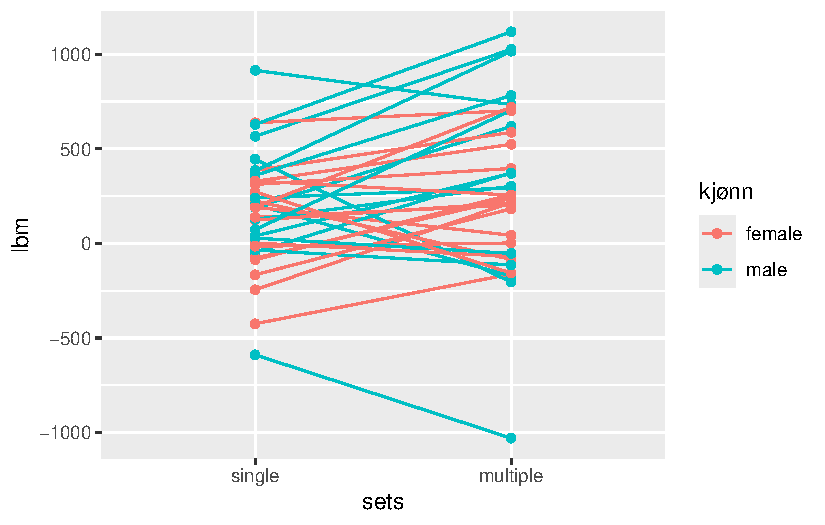
\includegraphics{Oppgave-5_files/figure-pdf/fig-lean-body-mass-1.pdf}

}

\caption{\label{fig-lean-body-mass}Forskjell på endring av muskelmasse
under intervensjonen mellom SSP og MSP hos manlige og kvinnelige
deltakere}

\end{figure}%

\subsubsection{Maksimal styrke}\label{maksimal-styrke}

Vi kan se en liknende tendens da det gjelder muskelstyrke. Den
gjennomsnitlige forskjellen i muskelstyrkeendring i beinpress mellom
sett-protokollene var 7.895kg CI: {[}1.1,14.6{]}, \emph{p}-value =0.025,
t30 =2.36) (95 \% konfidensintervall). Også her er det i gjennomsnitt en
større økning av 1RM ved MSP enn SSP. Men da vi ser på
Figure~\ref{fig-strength-test} kan vi også her se at resultatene
varierer hostetakerne. Her er det færre som har en klar fordel av MSP
selv om det er en tendens til det. Også her kan vi se at det er noen som
opplever en større økning ved SSP enn ved MSP.

\begin{figure}

\centering{

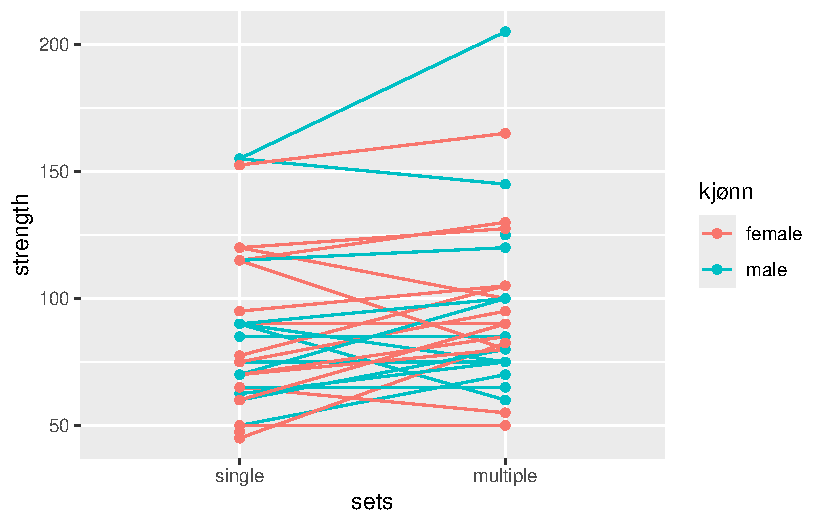
\includegraphics{Oppgave-5_files/figure-pdf/fig-strength-test-1.pdf}

}

\caption{\label{fig-strength-test}Forskjell på endring i styrke i
legpress under intervensjon mellom SSP og MSP hos mannlige og kvinnelige
deltakere}

\end{figure}%

\subsection{Diskusjon}\label{diskusjon-2}

I dette studiet fikk deltakerne en større økning i muskelmasse ved å
følge treningsprotokoll med flere sett (MSP) enn med et enkelt sett
(SSP). Dette stemmer over ens med anbefalingene fra (Anon, 2009) og
funnene til (Schoenfeld \emph{et al.}, 2016). Det som er overesakende i
denne studien er at det ikke var stor nok forskjell til å si at funnet
er statistisk signifikant med en \emph{p}-verdi på 0.036. Fra tabellen
kunne vi også se at noen deltakere ikke bare responderte like godt på
SSP som MSP, men faktisk bedre. Selv om vi ser en tendens til at det i
gjennomsnitt gir bedre effekt av MSP enn SSp kan vi altså ikke
konkludere med dette ut fra denne studien.

Vi får litt samme resultat i resultane for muskelstyrkeøknin (1RM). Også
her viser er det i gjennomsnitt en større økning i styrke ved MSP enn
ved SSP, men \emph{p}-verdien er enda lavere på 0,025, Så igjen er ikke
funnene signifikante. På styrke kan vi se at det er enda mindre
forskjell på effekten av SSP og MSP. Dette stemmer overens med studien
til (Mitchell \emph{et al.}, 2012) om at det kan være vanskelig å si hva
som gir best effekt av høyt og lavt treningsvolum.

Selv om vi ser en tendens i denne studien til at det totale utbyttet av
MSP er større enn SSP, er ikke forskjellen stor nok til å motbevise
null-hypotesen om at det ikke er noen forksjell. Den tendensen vi kan se
stemmer likevel med studien til (SCHOENFELD \emph{et al.}, 2019), hvor
de sier at treningsvolum er viktigere for hypertrofi enn for
muskelstyrke. Så kan vi likevel bruke funnene? (Naclerio \emph{et al.},
2013) sier i sin studie at selv om økt treningsvolum gir noe bedre
effekt er ikke dette alltid anbefalt for konkurrenrende utøvere på grunn
av det høye totalvolumet. Kanskje kan en liknende anbefaling gjelde for
utrente personer slik som deltakerne i denne studien. Denne studien
tyder på at lavt treningsvolum ikke har noen signifikant dårligere
effekt en høyt treningsvolum. At et sett per øvelse gir nesten like godt
resultat som tre vil være godt nytt for personer som sliter med
motivasjon eller som ikke liker styrketrening. Dette kan være svært
postitiv i et folkehelseperspektiv for å motivere flere til å trene og
holde seg i form med litt trening. Dette stemmer også med meta-studien
gjort av (Androulakis-Korakakis \emph{et al.}, 2019).

Vi kan altså ikke komme med noen klar konklusjon i denne studien. Det
var noe overraskende at hypotesen ikke stemte, spesielt med tanke på
hypertrofi. Det kan tenkes at det er en forskjell på trente og godt
trente i en slik situasjon så mer forskning innenfor dette feltet er nok
nødvendig. Selv om hypotesen ikke stemte kan det som sagt likevel være
positivt med tanke på folkehelse.

\bookmarksetup{startatroot}

\chapter{Filosofihistore}\label{filosofihistore}

(Okasha, 2016)

(Popper, 1969)

\section{Oppgave 2}\label{oppgave-2}

\begin{enumerate}
\def\labelenumi{\arabic{enumi}.}
\setcounter{enumi}{1}
\tightlist
\item
  \emph{Gi en kort beskrivelse av falsifikasjonisme og si litt om
  hvorfor Popper var motivert til å utvikle denne teorien. Presenter så
  ett problem med teorien og vurder hvorvidt problemet kan løses.}
\end{enumerate}

Karl Popper var enig med Humes filosofi om at induksjon var irrasjonelt
og at man ikke kan predikere framtid basert på fortid. Han mente også at
Humes induksjonsproblem var umulig å løse, og at induksjon rett og slett
var et mislykket prosjekt som ikke burde ha noe med vitenskap å gjøre.
Som et svar mot induksjon kom Popper med en deduktiv metode som kalles
«\emph{Falsifikasjonisme}». Kort forklart er dette en teori som sier at
vi aldri kan bevise em hypotese -- bare motbevise den, altså
falsifisere. Popper mente at alle vitenskapelige hypoteser må være
falsifiserbare. Dette vil ikke si at alle vitenskapelige teorier skal
være feil, men at det skal være mulig å forsøke og motbevise de gjennom
testing (Okasha, 2016).

Popper mente at flere såkalte vitenskapelige teorier ikke var
tilstrekkelig falsifiserbare til å kvalifiseres som vitenskap, men i
stedet var pseudo-vitenskap. Freuds psykoanalyse var en av teoriene
Popper ikke anerkjente som ekte vitenskap. Grunnen til dette var at
uansett hva en pasient gjorde eller led av kunne Freud forklare det med
teorien sin. Det var aldri noe som ikke passet inn i teorien og den
ville aldri bli motbevist. Ettersom den aldri kunne motbevises var den
ikke kvalifisert til å bli kalt vitenskap ifølge Popper (Okasha, 2016).
Et eksempel Popper selv bruker er at en mann dytter et barn ut i vannet
for å drukne det, og at en man hopper ut i vannet for å redde barnet.
Dette er motstridende handlinger som begge passer like godt i teoriene
til Freud og Adler, uten at teoriene motbevises. Dette mente Popper var
et bevis for svakhetene til teoriene deres, ikke styrkene (Popper,
1969).

Denne type teorier som aldri kunne motbevises, men alltid fant
bekreftende bevis var grunnen til at Popper kom med teorien om
falsifikasjonisme. Han mente som sagt at en hypotese bare var
vitenskapelig hvis den kunne falsifiseres. En vitenskapelig hypotese
skulle predikere noe -- gjerne så nøyaktig som mulig, og den skulle være
mulig å teste og eventuelt motbevises. Hvis et forsøk ikke klarte å
motbevise hypotesen var den ikke bekreftet, bare styrket. Eksempelet
Popper mente at all vitenskap burde strebe etter var Einsteins generelle
relativitetsteori. Her kom Einstein med en presis prediksjon om at
solens gravitasjon ville påvirke stråling fra stjerner. Dette ble senere
testet under en solformørkelse og observasjonene stemte med Einstein
prediksjon. Dette var akkurat det Popper mente var korrekt vitenskap --
en presis detaljert prediksjon som kunne testes (Popper, 1969).

En utfordring med Poppers teori om falsifikasjonisme er at den vil
utelukke, eller i alle fall gjøre det vanskelig for noen fagfelt å passe
inn i hans definisjon av vitenskap. I naturvitenskapelige fagfelt som
fysikk er det relativt enkelt å lage tester som skal forsøke å
falsifisere en hypotese. I psykologi for eksempel kan dette være langt
vanskeligere fordi det kan handle om hypoteser som ikke er målbare. Et
eksempel kan være følgende to påstander.

\begin{enumerate}
\def\labelenumi{\arabic{enumi}.}
\item
  Et barn vokser opp med en kriminell far. Barnet ser opp til faren sin
  og ønsker å bli som han. Barnet vil ende opp som kriminell selv.
\item
  Et barn vokser opp med en kriminell far. Barnet er flau over faren sin
  og han handlinger og ønsker å ta avstand fra det. Barnet vil ende opp
  som politi.
\end{enumerate}

Begge disse hypotesene er plausible, men det vil være umulig å lage en
test som motbeviser eller beviser de. Psykologi, personlighet, samfunn
og andre personer er variabler som er umulig å fjerne og som vil hindre
et eventuelt forsøk i å være reliabelt. Her kan vi bare vente å se på
oppveksten til barnet og så trekke en konklusjon etterpå slik som Freud
og Adler gjorde i sin tid. Dette vil ikke være særlig imponerende eller
vitenskapelig ifølge Popper, men det betyr ikke at påstandene er feil.

En mulig løsning på dette problemet er å kombinere deduksjon med
induksjon ved hjelp av statistikk og sannsynlighetsregning. I stedet for
å si med sikkerhet at 1: barnet vil bli kriminelt, eller 2: barnet vil
bli politi, kan man se på statistikk for barn som har vokst opp under
liknende forhold, og regne ut sannsynlighetene for hva som vil skje med
dette barnet. For eksempel 1: ut fra barnets oppvekst vil det være x \%
sannsynlig at barnet selv vil bli kriminelt, eller 2: ut fra barnets
oppvekst vil det være x \% sannsynlig at barnet vil ta avstand fra det
livet og bli politi. Det kan altså være mulig å kombinere deduksjon og
induksjon.

\bookmarksetup{startatroot}

\chapter{Labrapport; Ekstraksjon og analyse av
muskelprotein}\label{labrapport-ekstraksjon-og-analyse-av-muskelprotein}

\section{Introduksjon og bakgrunn}\label{introduksjon-og-bakgrunn}

I jakten på å bedre forstå de molekylære reaksjonene som er involvert i
reguleringen av transkripsjon og translasjon ved trening, ernæring,
sykdom og aldring, har også interessen og bruken av Western blot (WB)
innenfor treningsfysiologi økt. WB har flere bruksområder for
undersøkelse av regulatoriske molekylære reaksjoner, som for eksempel
kvantifisere proteinmengde og protein-protein-interaksjoner, som er
avgjørende for å kunne konstatere fysiologiske adaptasjoner til trening
(Bass \emph{et al.}, 2016) . Prosessen i WB deles inn i følgende steg:

\begin{enumerate}
\def\labelenumi{\arabic{enumi})}
\tightlist
\item
  Ekstraksjon av protein fra en sammensatt mikstur av intracellulær og
  ekstracellulær protein
\item
  Kvantifisering av proteinkonsentrasjon og elektroforese av protein
\item
  Overføring til en stabil membran med høg binding av proteiner
\item
  ``Blokking'' av membranen for å redusere bindingen av ikke-ønskede
  molekyl
\item
  Binding av antistoffer til de spesifikke proteinene man ønsker å
  undersøke
\item
  Binding av et sekundært antistoff, med en markør, til det første
  antistoffet
\item
  Utvikling og gjenkjenning av markøren
\item
  Kvantifisering av de resulterende båndene med hjelp av
  densiometriprogramvare
\end{enumerate}

Tidligere har WB kun blitt assosiert med selve prosessen med å overføre
proteinet fra en gel til en mer stabil membran, mens nå referer man til
WB når man skal forklare hele prosessen (Bass \emph{et al.}, 2016).

Formålet med vårt eksperimentet er å benytte seg av WB for å se på den
totale mengden av p70S6K (t-p70) og mengden fosforisert p70S6K fra
muskelvev. Med dette kan vi si noe om fosforyleringsnivået av p70S6K i
muskulaturen, som reflekterer hvor stor andel av p70S6K som er aktiv i
forhold til den totale proteinmengden i vevet. Muskelprøvene er hentet
fra høgre og venstre ben til ulike testpersoner, der alle har
gjennomgått styrketrening av de ene beinet ved ulike tidspunkt før selve
biopsien:

\begin{itemize}
\tightlist
\item
  Hennie (HE) = 10 min før biopsi
\item
  Lars (LØ) = 30 min før biopsi
\item
  Trond (T) = 60 min før biopsi
\end{itemize}

Prøven ble homogenisert forut for WB-analysen, som vil si at vi har
frigjort proteinene gjennom mekanisk eller kjemisk nedbryting av
cellemembranen. Selve protokollen og hvordan vi har utført
homogeniseringen og WB er beskrevet under, samt presentasjon og
diskusjon av resultatene.

\section{Metode}\label{metode-5}

\subsection{Homogenisering av
muskelprøver}\label{homogenisering-av-muskelpruxf8ver}

Vi benyttet oss av fryst vev av m.vastus lateralis som var blitt
ekstrahert fra både det høyre og venstre låret til en av
prøvedeltakerne. Vekten på de ulike prøvene var:

Høgre bein (HE-R): 14,0 μg Venstre bein (HE-L): 14,5 μg Til
homogenseringen benyttet vi oss av en plastpistill, og tilsatte 600 μl
med lysat-buffer som var satt sammen av 594 μl t-per og 6 μl pink for å
visualisere om vevet var fullstendig homogenisert.

For å måle proteinkonsentrasjonen i prøven vår, brukte vi Bradford
Assay-metoden. Denne metoden bruker et fargestoff, Coomassie Brilliant
Blue G-250, som vil binde seg til proteiner og skape en reaksjon der
prøven vil skifte farge til blå i proporsjon med proteinkonsentrasjonen
mengden protein. For å kvantifisere proteinkonsentrasjonen laget vi en
standardkurve med bovint serumalbumin som referanse, slik at vi kunne
sammenligne blåfargen i vår prøve med kjente proteinkonsentrasjoner. Vi
måler deretter, med hjelp av et spektrofotometer, hvor mye av prøvene
som blir absorbert ved 595 nm for å kunne bestemme om prøvene våre
inneholder lave eller høge konsentrasjoner av proteiner (Noble \&
Bailey, 2009). Protokollen under er en generell fremgangsmåte for
homogenisering av vev, og avvik og sentrale anmodninger er kommentert
under de ulike punktene.

Definisjoner: - BSA = Bovint serumalbumin, et protein som blir utvunne
fra blodplasmaet til storfe. Ofte brukt som standard for
proteinkonsentrasjon.

\subsubsection{Utstyrsliste}\label{utstyrsliste}

\begin{itemize}
\tightlist
\item
  Microfuge tubes (1.5 ml Eppendorf)
\item
  Plastic pestle
\item
  Centrifuge (capable of 10 000 g and 4°C)
\item
  Ice
\item
  Lysis buffer (e.g.~Hepes-buffer, Ripa-buffer)
\end{itemize}

\subsubsection{Protokoll}\label{protokoll-2}

\emph{Kursiv skrift}: Sentrale kommentarer fra selve utføringen.

\textbf{Fet skrift}: Mulige avvik

\begin{enumerate}
\def\labelenumi{\arabic{enumi}.}
\item
  Prepare the tissue by dissection away any connective tissue and blood.
  If you are working with wet tissue, this step should be done prior to
  freezing. Freeze dried tissue can be dissected in room temperature
  under the microscope. Use 10-50 mg wet-weight tissue or 2-10 mg
  freeze-dried tissue
\item
  Add protease/phosphatase inhibitors to the ice-cold lysis buffer (10
  μl/ml).
\end{enumerate}

\textbf{Pipetering mulig feilkilde i t-per, og i ene prøven (høyre)}

\begin{enumerate}
\def\labelenumi{\arabic{enumi}.}
\setcounter{enumi}{2}
\tightlist
\item
  Keep the sample on dry ice or cooling block until you add the ice cold
  lysis buffer of choice. Use 20 μl/mg wet-weight or 80 μl/mg dry
  weight.
\end{enumerate}

Dry: 2 mg → 160 μl, 5 mg → 400 μl, 10 mg → 800 μl

\begin{enumerate}
\def\labelenumi{\arabic{enumi}.}
\setcounter{enumi}{3}
\item
  Quickly disrupt the tissue by hand using the plastic pestle until
  there are no visible pieces.
\item
  Keep the sample on ice, vortex or rotate the sample for 20-60 min.
\end{enumerate}

\emph{Varighet av roteringen var 33min.}

\begin{enumerate}
\def\labelenumi{\arabic{enumi}.}
\setcounter{enumi}{5}
\item
  Spin the sample 10 min, 10 000 g, 4°C
\item
  Carefully remove the supernatant to a new tube without disrupting the
  pellet.
\item
  Aliquot the sample to a tube for protein concentration determination
  (1:10 dilution, 4 μl to 36 ul ddH2O. Keep a known volume for later
  normalization of the protein concentration (e.g.~to 3 ug/ul) keep on
  ice.
\end{enumerate}

\emph{Myo homogenat ofte utenfor standard. Bruker 1:6 fortynner for å
komme innenfor standard. 12 μl prøve og 60 μl vann.}

\emph{Pipetering gikk nokså bra også i dette leddet, liten sannsynlighet
for feilkilde, men skal aldri utelukkes.}

\begin{enumerate}
\def\labelenumi{\arabic{enumi}.}
\setcounter{enumi}{8}
\tightlist
\item
  Determine protein concentration with Bradford Assay. 10 μl sample +
  250 μl reagent. Make BSA (bovint serumalbumin) standards according to
  Thermo Sci guidelines (ref. 23209).
\end{enumerate}

\emph{Igjen ble pipeteringen godt utført, liten sannsynlighet for
feilkilder, men skal ikke utelukkes.}

\subsubsection{Mulige avvik:}\label{mulige-avvik}

\begin{itemize}
\tightlist
\item
  9.1.2, Punkt 2: Feil ved pipetering
\end{itemize}

\subsection{Western blot protokoll}\label{western-blot-protokoll}

Selv om gruppen jobbet med en prøve, er WB-analysen blitt gjort på flere
prøver fra 3 ulike testpersoner. For elektroforesen brukte vi Bio-Rad
Criterion og en ferdiglaget gel. Selv om det ikke ble brukt en
kalibreringskurve for å kvantifisere absolutt mengde p70S6K, ble
intensitetsverdiene normalisert mot total proteinmengde og deretter
brukt som en indikator for proteinaktivitet. Fosforyleringsnivået
(p−p70/t−p70p) ble beregnet for å gi et relativt mål på aktivering av
mTOR-signalveien.

\emph{Kursiv skrift}: Kommentarer fra utføringen \textbf{Fet skrift}:
Mulige avvik

\subsubsection{Løsninger}\label{luxf8sninger}

\begin{longtable}[]{@{}
  >{\raggedright\arraybackslash}p{(\columnwidth - 6\tabcolsep) * \real{0.1576}}
  >{\raggedright\arraybackslash}p{(\columnwidth - 6\tabcolsep) * \real{0.1330}}
  >{\raggedright\arraybackslash}p{(\columnwidth - 6\tabcolsep) * \real{0.3300}}
  >{\raggedright\arraybackslash}p{(\columnwidth - 6\tabcolsep) * \real{0.3793}}@{}}
\caption{\textbf{Løsninger}}\tabularnewline
\toprule\noalign{}
\begin{minipage}[b]{\linewidth}\raggedright
Buffer.Solution
\end{minipage} & \begin{minipage}[b]{\linewidth}\raggedright
Komponenter
\end{minipage} & \begin{minipage}[b]{\linewidth}\raggedright
Konsentrasjoner..mM.
\end{minipage} & \begin{minipage}[b]{\linewidth}\raggedright
Masser..g.
\end{minipage} \\
\midrule\noalign{}
\endfirsthead
\toprule\noalign{}
\begin{minipage}[b]{\linewidth}\raggedright
Buffer.Solution
\end{minipage} & \begin{minipage}[b]{\linewidth}\raggedright
Komponenter
\end{minipage} & \begin{minipage}[b]{\linewidth}\raggedright
Konsentrasjoner..mM.
\end{minipage} & \begin{minipage}[b]{\linewidth}\raggedright
Masser..g.
\end{minipage} \\
\midrule\noalign{}
\endhead
\bottomrule\noalign{}
\endlastfoot
TBS 1L 10x, pH 7.6 (HCl adjust) & Tris BaseNaCl & 20 mM x 10 = 200 mM137
mM x 10 = 1.37 M & 0.2 x 121.1 = 24.22 g1.37 x 58.44 = 80.06 g \\
Running buffer 1L 10x, pH 8.3 & Tris BaseGlycinSDS & 25 mM x 10 = 250
mM192 mM x 10 = 1.92 M3.5 mM x 10 = 35 mM & 0.25 x 121.1 = 30.28 g1.92 x
75.07 = 144.1 g0.035 x 288.38 = 10.09 g \\
Transfer buffer* 1L 10x & Tris BaseGlycin & 25 mM x 10 = 250 mM192 mM x
10 = 1.92 M & 0.25 x 121.1 = 30.28 g1.92 x 75.07 = 144.1 g \\
\end{longtable}

\begin{itemize}
\tightlist
\item
  1 x Transfer buffer = 100 ml TB stock x 10 + 100 ml methanol + 800 ml
  dH2O
\end{itemize}

\subsubsection{Sample preparation}\label{sample-preparation}

\begin{itemize}
\tightlist
\item
  Muscle samples should be prepared in an appropriate sample buffer
\item
  Dilute samples to a final concentration of 1.5-2 μg/μl in
  Laemmlibuffer (Bio-Rad)
\item
  Boil samples for 5 min, 95°C (denaturation). Cool to room temp. prior
  to loading. Spin down condensate
\end{itemize}

\subsubsection{Sample loading, gel
electrophoresis}\label{sample-loading-gel-electrophoresis}

\begin{itemize}
\item
  Assemble electrophoresis chamber on ice, add buffer to limit-mark
  \emph{(Det ble brukt Running buffer)}
\item
  Add protein ladder/standard (5 μl) \emph{(Proteinstige: Precision Plus
  Protein Dual Color Standards, 500 µl \#1610374)}, \emph{(Pipetering
  gikk fint)}
\item
  Load samples according to pre-written load scheme (max. Loading
  capacity in GTX precast gels: 30 μl) \textbf{(Pipeteringsfeil i brønn
  5: trakk prøven tilbake i pipetten en gang. Fikk alt ut igjen, men kan
  ha blitt blandet.)}, \emph{(Brønn 2-6 er p-p70 og brønn 9-13 er
  t-p70.)}
\end{itemize}

\begin{longtable}[]{@{}llllllllllllll@{}}
\toprule\noalign{}
1 & 2 & 3 & 4 & 5 & 6 & 7 & 8 & 9 & 10 & 11 & 12 & 13 & 14 \\
\midrule\noalign{}
\endhead
\bottomrule\noalign{}
\endlastfoot
M & H-L & H-R & T-L & T-R & L-R & M & M & H-L & H-R & T-L & T-R & L-R &
M \\
\end{longtable}

\begin{verbatim}
- M = Markør
- H-L = Hennie - Venstre ben
- H-R = Hennie - Høyre ben
- T-L = Trond - Venstre ben
- T-R = Trond - Høyre ben
- L-R = Lars - Høyre ben
\end{verbatim}

\begin{itemize}
\tightlist
\item
  Move electrophoresis chamber into 4 C. Top up buffer. Put on top lid.
\item
  Run gels: constant voltage, 30 min, 300 volt
\end{itemize}

\subsubsection{Protein transfer
(blotting)}\label{protein-transfer-blotting}

\begin{itemize}
\item
  Disassemble gels and place them in transferbuffer 15-30 min
\item
  Prepare sandwich:

  \begin{itemize}
  \tightlist
  \item
    Put sponges in dH2O to get rid of bubbles
  \item
    Put membranes (cut in upper left corner) in methanol to activate
    (5-10 min on shaker)
  \item
    Place sandwich in assembly tray -- black side down. Squeeze dH2O
    from sponges and place them in transferbuffer -- remove all bubbles
  \item
    Wet 2 filter papers in buffer, place them on top of gel and gently
    remove them together. Place filterpapers with gel on top of sponge.
    Remove bubbles
  \item
    Put membrane on top of gel. Careful with direction, membranes should
    be marked upper left corner. Remove bubbles
  \item
    Place the last sponge on top, close the sandwich
  \item
    Overføring til sandwich gikk fint, lav risiko for feilkilde.
  \end{itemize}
\item
  Place the sandwich in transfer tray
\item
  Run transfer: Constant ampere/current 300 mA, 3 h
\end{itemize}

\emph{Klippet hjørne på membran ved brønn 18.}

\textbf{Brukte hurtigprogram: 100V i 30 min.}

\subsubsection{Stain for total protein and cut
membrane}\label{stain-for-total-protein-and-cut-membrane}

\begin{itemize}
\tightlist
\item
  Mix destain solution with methanol 1:1 \emph{(30:30 ml)}
\item
  Mix Eraser solution with methanol 1:1 \emph{(30:30 ml)}
\item
  Rinse the membrane quickly in dH2O
\item
  Add MemCode Sensitizer to the the membrane, place on shaker for 2 min.
  Decant solution,
\end{itemize}

reuse 1 time

\begin{itemize}
\tightlist
\item
  Add MemCode Reversible stain, on shaker 1 min. Decant. Reuse 1 time.
\item
  Destain by adding MemCode destain to membrane, rinse quickly 3 times
\item
  Add methanol/destain solution, on shaker, 5 min- Rinse with dH2O 4
  times\#
\item
  Image membrane
\item
  Cut the membrane. If multiple membranes, number each
\item
  Proceed with Eraser → Add eraser/methanol solution to the membrane on
  shaker, 10 min*
\item
  Rinse the membrane in dH2O 4 times. Store in TBS until cut
\item
  Cut membranes according to protein weight and/or wells used
\end{itemize}

\subsubsection{Blocking and primary
antibody}\label{blocking-and-primary-antibody}

\begin{itemize}
\tightlist
\item
  Block the membrane in 2,5 \% milk in TBS-T for 1 h at room temp
\item
  Decant blocking solution, rinse in TBS
\item
  Add primary antibody (AB) in BSA/milk solution (5\% in TBS-T),
  incubate over night in 4 C
\end{itemize}

\textbf{Brukte 5 \% milk i TBS-T}

\subsubsection{Antibody wash and secondary
antibody}\label{antibody-wash-and-secondary-antibody}

\textbf{Denne delen ble gjort av Vilde, og vi har derfor ikke oversikt
over mulige avvik her, men har spesifisert muligheter for avvik under}

\begin{itemize}
\tightlist
\item
  Wash with TBS-T 2x1 min + 3x5 min \textbf{(Unøyaktig vasking vil kunne
  føre til bakgrunnsstøy.)}
\item
  Add secondary AB in 2,5\% milk with TBS-T for 1 h at room temp
\item
  Wash with TBS 4x5 min \textbf{(Unøyaktig vasking vil kunne føre til
  bakgrunnsstøy.)}
\item
  Perform ECL

  \begin{itemize}
  \tightlist
  \item
    Mix working solution (Thermo super signal \ldots)
  \item
    Incubate membrane for 5 min at room temp
  \item
    Cover blot in clear plastic wrap
  \end{itemize}
\item
  Collect image on Gel Doc
\end{itemize}

\subsubsection{Mulige avvik:}\label{mulige-avvik-1}

\begin{itemize}
\tightlist
\item
  Punkt 7.2.2.3: Pipeteringsfeil i brønn 5: trakk prøven tilbake i
  pipetten en gang. Fikk alt ut igjen, men kan ha blitt blandet.
\item
  Punkt 7.2.2.4: Brukte hurtigprogram: 100V i 30 min.
\item
  Punkt 7.2.2.7: En annen person utførte vaskingen - derfor ikke
  kontroll over dette.
\end{itemize}

\section{Resultater}\label{resultater-1}

Vi benyttet oss av WB-analyse for å kvantifisere total p70S6K og
fosforlyert p70S6K, slik at vi kunne undersøke fosforyleringsnivået til
proteinet i vastus lateralis til de ulike testpersonene. Intensiteten
til fosforylert p70S6K (p-p70) og total p70S6K (t-p70) ble normalisert
mot totalprotein fra membran blottet. Fosforyleringsnivået ble beregnet
som forholdet mellom p-p70 og t-70 (p-p70 / t-p70). Intensitetsverdiene
som presenteres i tabellene er basert på optisk tetthet fra Western
blot-bildene. Verdiene representerer relative signalstyrker og har ingen
absolutt måleenhet, da kalibreringskurve ikke ble benyttet. For å
korrigere for variasjoner i proteinmengde mellom brønnene, f.eks grunnet
pipeteringsfeil eller feil i total protein-målinger, ble intensitetene
normalisert mot total proteinmengde (membran blot).

I Tabell 1 vises de normaliserte intensitetsverdiene for fosforylert
(p-p70) og total (t-p70) p70S6K for høyre og venstre bein hos hver
testperson, basert på membran blottet. Fosforyleringsnivået er beregnet
som forholdet mellom normalisert p-p70 og t-p70. Fosforyleringsnivået
(p-p70/t-p70) varierte mellom prøvene, med høyest nivå i høyre bein hos
testperson T (1.550) og lavest i venstre bein hos testperson LØ (0.920).

\begin{longtable}[]{@{}
  >{\raggedright\arraybackslash}p{(\columnwidth - 16\tabcolsep) * \real{0.0833}}
  >{\raggedright\arraybackslash}p{(\columnwidth - 16\tabcolsep) * \real{0.0606}}
  >{\raggedright\arraybackslash}p{(\columnwidth - 16\tabcolsep) * \real{0.1591}}
  >{\raggedright\arraybackslash}p{(\columnwidth - 16\tabcolsep) * \real{0.1591}}
  >{\raggedright\arraybackslash}p{(\columnwidth - 16\tabcolsep) * \real{0.0909}}
  >{\raggedright\arraybackslash}p{(\columnwidth - 16\tabcolsep) * \real{0.0909}}
  >{\raggedright\arraybackslash}p{(\columnwidth - 16\tabcolsep) * \real{0.1061}}
  >{\raggedright\arraybackslash}p{(\columnwidth - 16\tabcolsep) * \real{0.1061}}
  >{\raggedright\arraybackslash}p{(\columnwidth - 16\tabcolsep) * \real{0.1439}}@{}}
\caption{\textbf{Oppsummering av absolutte verdier til de individuelle
testpersonene}}\tabularnewline
\toprule\noalign{}
\begin{minipage}[b]{\linewidth}\raggedright
Testperson
\end{minipage} & \begin{minipage}[b]{\linewidth}\raggedright
Bein
\end{minipage} & \begin{minipage}[b]{\linewidth}\raggedright
Membran.blot..p.p70.
\end{minipage} & \begin{minipage}[b]{\linewidth}\raggedright
Membran.blot..t.p70.
\end{minipage} & \begin{minipage}[b]{\linewidth}\raggedright
p.p70..raw.
\end{minipage} & \begin{minipage}[b]{\linewidth}\raggedright
t.p70..raw.
\end{minipage} & \begin{minipage}[b]{\linewidth}\raggedright
p.p70..norm..
\end{minipage} & \begin{minipage}[b]{\linewidth}\raggedright
t.p70..norm..
\end{minipage} & \begin{minipage}[b]{\linewidth}\raggedright
Fosforyleringsnivå
\end{minipage} \\
\midrule\noalign{}
\endfirsthead
\toprule\noalign{}
\begin{minipage}[b]{\linewidth}\raggedright
Testperson
\end{minipage} & \begin{minipage}[b]{\linewidth}\raggedright
Bein
\end{minipage} & \begin{minipage}[b]{\linewidth}\raggedright
Membran.blot..p.p70.
\end{minipage} & \begin{minipage}[b]{\linewidth}\raggedright
Membran.blot..t.p70.
\end{minipage} & \begin{minipage}[b]{\linewidth}\raggedright
p.p70..raw.
\end{minipage} & \begin{minipage}[b]{\linewidth}\raggedright
t.p70..raw.
\end{minipage} & \begin{minipage}[b]{\linewidth}\raggedright
p.p70..norm..
\end{minipage} & \begin{minipage}[b]{\linewidth}\raggedright
t.p70..norm..
\end{minipage} & \begin{minipage}[b]{\linewidth}\raggedright
Fosforyleringsnivå
\end{minipage} \\
\midrule\noalign{}
\endhead
\bottomrule\noalign{}
\endlastfoot
HE & Venstre & 16530.472 & 15516.16 & 4276.447 & 4276.447 & 0.2587 &
0.2756 & 0.939 \\
HE & Høyre & 10135.430 & 13009.67 & 4238.276 & 4238.276 & 0.4182 &
0.3257 & 1.284 \\
T & Venstre & 11187.966 & 12917.48 & 4457.276 & 4457.276 & 0.3985 &
0.3449 & 1.155 \\
T & Høyre & 7012.388 & 10868.74 & 4148.447 & 4148.447 & 0.5916 & 0.3816
& 1.550 \\
L & Høyre & 14791.037 & 13617.43 & 4249.861 & 4249.861 & 0.2872 & 0.3122
& 0.920 \\
\end{longtable}

Den gjennomsnittlige aktiviteten til p70S6K på tvers av gruppen var
1.168 ± 0.248, med et høyere nivå i høyre bein (1.426 ± 0.147)
sammenlignet med venstre bein (0.986 ± 0.090). Variasjonen i
fosforyleringsnivået var høyest på gruppenivå med en CV på 21.23\%, og
lavere når høyre (CV = 10.31\%) og venstre bein ble analysert separat
(CV = 9.13\%).

\begin{longtable}[]{@{}
  >{\raggedright\arraybackslash}p{(\columnwidth - 6\tabcolsep) * \real{0.1284}}
  >{\raggedright\arraybackslash}p{(\columnwidth - 6\tabcolsep) * \real{0.2905}}
  >{\raggedright\arraybackslash}p{(\columnwidth - 6\tabcolsep) * \real{0.2905}}
  >{\raggedright\arraybackslash}p{(\columnwidth - 6\tabcolsep) * \real{0.2905}}@{}}
\caption{\textbf{Gjennomsnittlige nivåer av total og fosforylert p70S6K,
samt forskjellen mellom disse, i høyre og venstre bein. Presenteres som
gjennomsnitt (gj.snitt), standardavvik (SD) og coefficient of variation
(CV) }}\tabularnewline
\toprule\noalign{}
\begin{minipage}[b]{\linewidth}\raggedright
Parameter
\end{minipage} & \begin{minipage}[b]{\linewidth}\raggedright
Hele.gruppen..n\ldots20.
\end{minipage} & \begin{minipage}[b]{\linewidth}\raggedright
Høyre.bein..n\ldots10.
\end{minipage} & \begin{minipage}[b]{\linewidth}\raggedright
Venstre.bein..n\ldots10.
\end{minipage} \\
\midrule\noalign{}
\endfirsthead
\toprule\noalign{}
\begin{minipage}[b]{\linewidth}\raggedright
Parameter
\end{minipage} & \begin{minipage}[b]{\linewidth}\raggedright
Hele.gruppen..n\ldots20.
\end{minipage} & \begin{minipage}[b]{\linewidth}\raggedright
Høyre.bein..n\ldots10.
\end{minipage} & \begin{minipage}[b]{\linewidth}\raggedright
Venstre.bein..n\ldots10.
\end{minipage} \\
\midrule\noalign{}
\endhead
\bottomrule\noalign{}
\endlastfoot
t-p70 (norm.) & Gj.sn: 0.3280SD: 0.0366CV = 11.16\% & Gj.sn: 0.3537SD:
0.0396CV = 11.19\% & Gj.sn: 0.3127SD: 0.0298CV = 9.53\% \\
p-p70 (norm.) & Gj.sn: 0.3908SD: 0.1174CV = 30.04\% & Gj.sn: 0.5049SD:
0.1227CV = 24.30\% & Gj.sn: 0.3148SD: 0.0704CV = 22.37\% \\
Fosforyleringsnivå & Gj.sn: 1.168SD: 0.248CV = 21.23\% & Gj.sn: 1.426SD:
0.147CV = 10.31\% & Gj.sn: 0.986SD: 0.090CV = 9.13\% \\
\end{longtable}

\section{Diskusjon}\label{diskusjon-3}

Intensitetsverdiene gir oss et bilde av p70S6K-aktiviteten i prøvene, og
selv om absolutt kvantifisering ikke ble utført, indikerer et høyere
fosforyleringsnivå en økt aktivitet av mTOR-signalveien, som spiller en
viktig rolle for proteinsyntesen. Det høyere fosforyleringsnivået i
høyre bein (1.4261) sammenlignet med venstre (0.986) kan forklares ved
at kun det ene beinet ble trent før biopsien. Dette viser til den akutte
aktiveringen av mTOR-signalveien som respons av styrketrening, der den
største aktiveringen ser ut til å forekomme kort tid etter trening, med
en gradvis reduksjon over tid. Et høyere fosforyleringsnivå reflekterer
potensielt et større kapasitet for proteinsyntese i det trente beinet.
Nivå over 1.0 i flere prøver kan tyde på høy aktivering av p70S6K, men
kan også være et resultat av tekniske faktorer.

Høyere variasjon i fosforylert p70S6K (CV = 30.04 \%) sammenlignet med
total p70S6K (CV = 11.16 \%) kan skyldes biologisk variasjon i
mTOR-signalveien mellom testpersoner. Samtidig kan tekniske faktorer som
variasjoner i prøvehåndtering ha bidratt til dette. Lavere CV i høyre
(10.31\%) og venstre bein (9.13\%) indikerer mer konsistens når prøvene
analyseres separat.

\section{Konklusjon}\label{konklusjon}

Den asymmetriske aktiveringen av mTOR-signalveien mellom høyre og
venstre bein kan forklares ved at kun det ene beinet ble trent før
biopsien. Resultatene viser hvordan styrketrening kan gi en akutt økning
i fosforyleringsnivået av p70S6K, med størst aktivering observert kort
tid etter trening. Resultatene burde likevel tolkes med omhu, da
tekniske faktorer som bakgrunnsstøy på blottet, feil pipettering, ujevn
proteinoverføring, manglende kalibrerintgskurve kan ha påvirket
intensitetsmålingene.

\bookmarksetup{startatroot}

\chapter*{Kilder}\label{kilder}
\addcontentsline{toc}{chapter}{Kilder}

\phantomsection\label{refs}
\begin{CSLReferences}{1}{1}
\bibitem[\citeproctext]{ref-almquist2022}
Almquist NW, Eriksen HB, Wilhelmsen M, Hamarsland H, Ing S, Ellefsen S,
Sandbakk Ø, Rønnestad BR \& Skovereng K (2022). No differences between
12{\hspace{0.167em}}weeks of block- vs. Traditional-periodized training
in performance adaptations in trained cyclists. \emph{Frontiers in
Physiology}; DOI:
\href{https://doi.org/10.3389/fphys.2022.837634}{10.3389/fphys.2022.837634}.

\bibitem[\citeproctext]{ref-androulakis-korakakis2019}
Androulakis-Korakakis P, Fisher JP \& Steele J (2019).
\href{https://doi.org/10.1007/s40279-019-01236-0}{The Minimum Effective
Training Dose Required to Increase 1RM Strength in Resistance-Trained
Men: A Systematic Review and Meta-Analysis}. \emph{Sports Medicine}
\textbf{50,} 751--765.

\bibitem[\citeproctext]{ref-progress2009}
Anon (2009).
\href{https://doi.org/10.1249/mss.0b013e3181915670}{Progression Models
in Resistance Training for Healthy Adults}. \emph{Medicine \& Science in
Sports \& Exercise} \textbf{41,} 687--708.

\bibitem[\citeproctext]{ref-R}
Anon (n.d.). \emph{R: A language and environment for statistical
computing}.

\bibitem[\citeproctext]{ref-bass2016}
Bass JJ, Wilkinson DJ, Rankin D, Phillips BE, Szewczyk NJ, Smith K \&
Atherton PJ (2016). \href{https://doi.org/10.1111/sms.12702}{An overview
of technical considerations for Western blotting applications to
physiological research}. \emph{Scandinavian Journal of Medicine \&
Science in Sports} \textbf{27,} 4--25.

\bibitem[\citeproctext]{ref-lme4}
Bates D, Mächler M, Bolker B \& Walker S (2015). Fitting linear
mixed-effects models using {\textbraceleft}lme4{\textbraceright}. ; DOI:
\href{https://doi.org/10.18637/jss.v067.i01}{10.18637/jss.v067.i01}.

\bibitem[\citeproctext]{ref-breil2010}
Breil FA, Weber SN, Koller S, Hoppeler H \& Vogt M (2010).
\href{https://doi.org/10.1007/s00421-010-1455-1}{Block training
periodization in alpine skiing: effects of 11-day HIT on VO2max and
performance}. \emph{European Journal of Applied Physiology}
\textbf{109,} 1077--1086.

\bibitem[\citeproctext]{ref-brosowsky2020}
Brosowsky N, Parshina O, Locicero A \& Crump MJC (2020). Teaching
undergraduate students to read empirical articles: An evaluation and
revision of the QALMRI method. Available at:
\url{http://dx.doi.org/10.31234/osf.io/p39sc}.

\bibitem[\citeproctext]{ref-halperin2015}
Halperin I, Pyne DB \& Martin DT (2015).
\href{https://doi.org/10.1123/ijspp.2014-0566}{Threats to internal
validity in exercise science: A review of overlooked confounding
variables}. \emph{Int J Sports Physiol Perform} \textbf{10,} 823--829.

\bibitem[\citeproctext]{ref-hopkins2000}
Hopkins WG (2000).
\href{http://www.ncbi.nlm.nih.gov/pubmed/10907753}{Measures of
reliability in sports medicine and science}. \emph{Sports Med}
\textbf{30,} 1--15.

\bibitem[\citeproctext]{ref-hulley2013}
Hulley SB, Cummings SR, Browner WS, Grady DG \& Newman TB (2013).
Designing clinical research - fourth edition. \emph{LIPPINCOTT WILLIAMS
\& WILKINS, a WOLTERS KLUWER business}. Available at:
\url{file:///C:/Users/Anders\%20Nybakk/OneDrive/Skrivebord/Kvantitativ\%20metode\%20og\%20statistik/Hulley\%20(2013)\%20-\%20Designingclinicalresearch_4th-edition.pdf}.

\bibitem[\citeproctext]{ref-javaloyes2020}
Javaloyes A, Sarabia JM, Lamberts RP, Plews D \& Moya-Ramon M (2020).
\href{https://doi.org/10.1519/jsc.0000000000003337}{Training
Prescription Guided by Heart Rate Variability Vs. Block Periodization in
Well-Trained Cyclists}. \emph{Journal of Strength and Conditioning
Research} \textbf{34,} 1511--1518.

\bibitem[\citeproctext]{ref-machado2012}
Machado FA, Nakamura FY \& Moraes SMFD (2012). Influence of regression
model and incremental test protocol on the relationship between lactate
threshold using the maximal-deviation method and performance in female
runners. \emph{Journal of sports sciences} \textbf{30,} 1267--1274.

\bibitem[\citeproctext]{ref-mcardle2014}
McArdle WD, Katch FI \& Katch VL (2014). \emph{Exercise physiology:
Nutrition, energy, and human performance}, 8th edn. Wolters Kluwer
Health.

\bibitem[\citeproctext]{ref-mitchell2012}
Mitchell CJ, Churchward-Venne TA, West DWD, Burd NA, Breen L, Baker SK
\& Phillips SM (2012).
\href{https://doi.org/10.1152/japplphysiol.00307.2012}{Resistance
exercise load does not determine training-mediated hypertrophic gains in
young men}. \emph{Journal of Applied Physiology} \textbf{113,} 71--77.

\bibitem[\citeproctext]{ref-naclerio2013}
Naclerio F, Faigenbaum AD, Larumbe-Zabala E, Perez-Bibao T, Kang J,
Ratamess NA \& Triplett NT (2013).
\href{https://doi.org/10.1519/jsc.0b013e3182736d10}{Effects of Different
Resistance Training Volumes on Strength and Power in Team Sport
Athletes}. \emph{Journal of Strength and Conditioning Research}
\textbf{27,} 1832--1840.

\bibitem[\citeproctext]{ref-noble2009}
Noble JE \& Bailey MJA (2009). Chapter 8 quantitation of protein. In,
pp. 73--95. Elsevier. Available at:
\url{http://dx.doi.org/10.1016/S0076-6879(09)63008-1}.

\bibitem[\citeproctext]{ref-okasha2016}
Okasha S (2016). \emph{Philosophy of science - a very short
introduction}, 2nd edn. Oxford University Press.

\bibitem[\citeproctext]{ref-pauw2013}
Pauw KD, Roelands B, Cheung SS, Geus B de, Rietjens G \& Meeusen R
(2013). \href{https://doi.org/10.1123/ijspp.8.2.111}{Guidelines to
classify subject groups in sport-science research}. \emph{International
Journal of Sports Physiology and Performance} \textbf{8,} 111--122.

\bibitem[\citeproctext]{ref-popper1969}
Popper K (1969). \emph{Conjectures and refutations : The growth of
scientific knowledge}, 1rst edn. Routledge; Kegan Paul.

\bibitem[\citeproctext]{ref-ruxf8nnestad2012a}
Rønnestad BR, Ellefsen S, Nygaard H, Zacharoff EE, Vikmoen O, Hansen J
\& Hallén J (2012\emph{a}).
\href{https://doi.org/10.1111/sms.12016}{Effects of 12 weeks of block
periodization on performance and performance indices in well{-}trained
cyclists}. \emph{Scandinavian Journal of Medicine \& Science in Sports}
\textbf{24,} 327--335.

\bibitem[\citeproctext]{ref-ruxf8nnestad2012}
Rønnestad BR, Hansen J \& Ellefsen S (2012\emph{b}).
\href{https://doi.org/10.1111/j.1600-0838.2012.01485.x}{Block
periodization of high{-}intensity aerobic intervals provides superior
training effects in trained cyclists}. \emph{Scandinavian Journal of
Medicine \& Science in Sports} \textbf{24,} 34--42.

\bibitem[\citeproctext]{ref-ruple2023}
Ruple BA, Plotkin DL, Smith MA, Godwin JS, Sexton CL, McIntosh MC,
Kontos NJ, Beausejour JP, Pagan JI, Rodriguez JP, Sheldon D, Knowles KS,
Libardi CA, Young KC, Stock MS \& Roberts MD (2023). The effects of
resistance training to near failure on strength, hypertrophy, and motor
unit adaptations in previously trained adults. \emph{Physiological
Reports}; DOI:
\href{https://doi.org/10.14814/phy2.15679}{10.14814/phy2.15679}.

\bibitem[\citeproctext]{ref-schoenfeld2019}
SCHOENFELD BJ, CONTRERAS B, KRIEGER J, GRGIC J, DELCASTILLO K, BELLIARD
R \& ALTO A (2019).
\href{https://doi.org/10.1249/mss.0000000000001764}{Resistance Training
Volume Enhances Muscle Hypertrophy but Not Strength in Trained Men}.
\emph{Medicine \& Science in Sports \& Exercise} \textbf{51,} 94--103.

\bibitem[\citeproctext]{ref-schoenfeld2016}
Schoenfeld BJ, Pope ZK, Benik FM, Hester GM, Sellers J, Nooner JL,
Schnaiter JA, Bond-Williams KE, Carter AS, Ross CL, Just BL, Henselmans
M \& Krieger JW (2016).
\href{https://doi.org/10.1519/jsc.0000000000001272}{Longer Interset Rest
Periods Enhance Muscle Strength and Hypertrophy in Resistance-Trained
Men}. \emph{Journal of Strength and Conditioning Research} \textbf{30,}
1805--1812.

\bibitem[\citeproctext]{ref-spiegelhalter2019}
Spiegelhalter D (2019\emph{a}). The art of statistics: How to learn from
data. \emph{New York: Basic books, Hatchet book group}.

\bibitem[\citeproctext]{ref-spieg2019}
Spiegelhalter DJ (2019\emph{b}). \emph{The art of statistics : Learning
from data}, 1th edn. Pelican.

\bibitem[\citeproctext]{ref-tanner2012}
Tanner RK \& Gore CJ (2012). \emph{Physiological tests for elite
athletes}, 2nd edn. Human Kinetics. Available at:
\url{https://books.google.no/books?id=0OPIiMks58MC}.

\bibitem[\citeproctext]{ref-wackerhage2014}
Wackerhage H (2014). \emph{Molecular exercise physiology - an
introduction}, 1rst edn. Routledge.

\bibitem[\citeproctext]{ref-walker2024}
Walker O (2024). Heart rate variability (HRV). \emph{Science for Sport}.
Available at:
\url{https://www.scienceforsport.com/heart-rate-variability-hrv/}.

\end{CSLReferences}




\end{document}
